
\setchapterpreamble[ur]{%
\dictum[G.~Box~\cite{box1987empirical}]{%
All models are wrong, but some are useful.}%
\vspace*{2\baselineskip}}

%%%%%%%%%%%%%%%%%%%%%%%%%%%%%%%%%%%%%%%%%%%%%%%%%%%%%%%%%%%%
\chapter{Higgs effective theory at its limits}
\label{chapter:validity}
%%%%%%%%%%%%%%%%%%%%%%%%%%%%%%%%%%%%%%%%%%%%%%%%%%%%%%%%%%%%



%%%%%%%%%%%%%%%%%%%%%%%%%%%%%%%%%%%%%%%%%%%%%%%%%%%%%%%%%%%%
\section{Introduction}
%%%%%%%%%%%%%%%%%%%%%%%%%%%%%%%%%%%%%%%%%%%%%%%%%%%%%%%%%%%%

The Higgs boson~\cite{Higgs:1964ia, Higgs:1964pj, Englert:1964et}
discovery announced on July 4th 2012~\cite{Aad:2012tfa,
  Chatrchyan:2012xdj} is a historical milestone in the physics of the
21st century.  The thorough scrutiny of the LHC Run I data has so far
confirmed that the narrow resonance observed at a mass around 125~GeV
is compatible with the minimal Standard Model (SM) agent of
electroweak symmetry breaking~\cite{Plehn:2009nd}. To date, this
agreement is limited to around $20\%$ precision in the Higgs
couplings~\cite{Lafaye:2009vr, Corbett:2012ja, Klute:2012pu,
  Dobrescu:2012td, Cheung:2013kla, Giardino:2013bma, Chang:2013cia,
  Djouadi:2013qya, Corbett:2015ksa}, which is not sensitive to the
deviations that one would expect from typical perturbatively extended
Higgs sectors.  This accuracy, based on a large set of on-shell and
most recently off-shell Higgs measurements~\cite{Corbett:2015ksa}, will
soon improve with data from Run~II.  Odds are high that the upcoming
runs will shed light on a possible UV completion of the Standard
Model~\cite{Englert:2014uua, Morrissey:2009tf}.

Based on everything we know, such an underlying theory should be
described by a gauge field theory. While the measurement of Higgs
couplings from inclusive rates has been extremely successful at Run~I,
it needs to be extended, for example to include kinematic
distributions. For this purpose, Higgs effective field theories
(EFT)~\cite{Weinberg:1980wa, Coleman:1969sm, Callan:1969sn,
  Burges:1983zg, Leung:1984ni, Buchmuller:1985jz} have become the
\emph{koin\'e} for discussing the phenomenology of extended Higgs
sectors.  In the effective field theory language, beyond the Standard
Model (BSM) effects are described in terms of a Lagrangian with local
operators of increasing mass dimension $d > 4$. Each of them includes
a suppression by inverse powers of a new physics scale, which should
be well separated from the experimentally accessible scale, in our
case the electroweak scale, $\Lambda \gg v$.

Despite its generality, the EFT approach is known to suffer from its
limited applicability when the hierarchy of scales is not guaranteed.
This has fueled intense investigation in the context of dark matter
searches~\cite{dm}.  While in that field EFT-based predictions are
usually robust for early-universe and late-time annihilation rates as
well as for dark matter-nucleon scattering, the required hierarchy of
scales can break down for dark matter signals at colliders. Because
hadron collider do not have a well-defined partonic energy, strategies
relying on boosted objects and large recoils are the most
critical. While it is not clear that a marginal separation of scales
invalidates the EFT approach, such observables clearly pose a
challenge.\medskip

There exists a first set of studies of the applicability of EFTs to
Higgs physics at the
LHC~\cite{Biekoetter:2014jwa,heft_limitations,heft_limitations2}.
These questions first arose in studies of tagging jet kinematics in
weak boson fusion, which are sensitive to the UV structure of the
theory~\cite{bad_one,spins,phi_jj,higgs_pole}. Similar issues appear
in Higgs-strahlung~\cite{Biekoetter:2014jwa} and in the production of
off-shell Higgs bosons in gluon
fusion~\cite{taming,Buschmann:2014sia}. A key problem is that Higgs
production at hadron colliders does not probe a single energy scale
over the full relevant phase space.

On the other hand, in Ref.~\cite{Corbett:2015ksa} is has been shown that
a fit of dimension-6 operators to the Higgs data at Run~I is a
sensible and practicable extension of the usual Higgs couplings fit.
Dimension-6 operators including derivatives complement the Higgs
coupling modifications and allow us to extract information from
kinematic distributions. Because the LHC constraints do not induce a
hierarchy of scales, the EFT approach is not formally well
defined. However, there appears to be no problem in describing the LHC
Higgs data in terms of a truncated dimension-6 Lagrangian. This
description induces theory uncertainties if we want to interpret the
LHC results in terms of an effective field theory~\cite{trott}. On the
other hand, these and other theory uncertainties can and should be
separated from the experimental
uncertainties~\cite{Cranmer:2013hia,fichet_moreau}.

Related to the topic of the validity of the effective theory is the
question if, given the experimental performance, the analysis of a
UV-complete model offers an advantage compared to the effective
theory~\cite{Henning:2014wua}. The two approaches are only equivalent
if we account for the full correlations between the effective
operators in all analysis steps, and if the effective theory is
applicable over the full relevant phase space. Unless the experimental
collaborations provide their fully correlated results beyond a
Gaussian approximation~\cite{Corbett:2015ksa}, a direct analysis of full
models will be superior.\medskip

Given these arguments, the applicability of the dimension-6
description of the Higgs sector has to be tested on a
process-to-process as well as model-to-model basis.  In this paper we
present a comprehensive comparison of full models and their truncated
EFT description during the LHC Run~II. We select extensions of the
Higgs sector of the Standard Model by \textit{i)} a scalar singlet,
\textit{ii)} a scalar doublet, \textit{iii)} a colored top-partner
scalar, and \textit{iv)} a massive vector triplet.  Each of these
models is mapped onto an EFT, which we obtain by integrating out the
heavy fields and expanding the operators to dimension 6. We then
derive predictions for selected Higgs observables in the full model
and compare them to the EFT results.  The key questions we aim to
address are:
%
\begin{enumerate}
\item Given the LHC sensitivity, how large do relevant new physics
effects have to be?
\item Does the corresponding new physics scale respect a
self-consistency condition $\Lambda \gg v$?
\item Which observables are correctly described by the truncated EFT?
\item What are the reasons for the potential failure of this EFT?
\item Do they pose a problem for LHC analyses?
\end{enumerate}
%
For weakly interacting models, visible effects at the LHC lead us to
scenarios in which the heavy scale is not sufficiently separated from
the electroweak scale, and the EFT description is not obviously
justified. We will analyze what problems the lack of a clear hierarchy
of scales leads to in practice, and discuss how these might affect
global LHC-Higgs fits including kinematic
distributions~\cite{Corbett:2015ksa}.

It will turn out that two limitations of the EFT description will
guide us through the different models. First, we need to ensure that
the new physics scale and with it all new particles are properly
decoupled, in particular when we go beyond total cross
sections. Second, when we define our effective field theory in terms
of a Higgs-Goldstone doublet, it is crucial that the electroweak
vacuum expectation value (VEV) does not have a destabilizing effect on
the hierarchy of scales.\medskip

The remainder of the paper is organized as follows: in
Section~\ref{sec:validity_theory} we review our theoretical framework. We
discuss how new physics effects in the Higgs sector are accounted for
in the full model and EFT languages, and we identify the reasons why
the two methods can deviate from each other.  In
Section~\ref{sec:validity_analysis} we show these ideas at work by explicitly
confronting full model versus EFT predictions for a variety of UV
completions and Higgs observables.  We give our conclusions in
Section~\ref{sec:validity_summary}. We hope that the
Appendices~\ref{sec:validity_ap-eft}\,--\,\ref{sec:validity_ap-triplet} with exhaustive
details on the different models and their EFT parametrizations will be
particularly useful to practitioners.



%%%%%%%%%%%%%%%%%%%%%%%%%%%%%%%%%%%%%%%%

After the discovery of a light Higgs boson~\cite{higgs,discovery}, one
of the key tasks of the LHC is to test if the observed particle indeed
corresponds to the minimalist setup of the Higgs sector in the
Standard Model. Because of the many intricacies of the electroweak
sector of the Standard Model, it is not straightforward to define a
theoretical framework which describes possible deviations in the Higgs
sector. If we want to remain more general than testing specific
models~\cite{bsmreview}, we can use an effective field theory ansatz.
Here the Lagrangian is organized by the field or particle content, the
symmetry structure, and the mass
dimension~\cite{eftfoundations,eftorig,higgsreview}.

The problem at least for the interpretation of Run~I results in terms
of an effective theory is that the experimental accuracy does not
translate into a hierarchy of scales~\cite{legacy,heft_limitations}.
For total rate measurements at the LHC this can be seen easily: if we
assume that the higher-dimensional operators are ordered by factors
$g^2 m_h^2/\Lambda^2$, a typical LHC accuracy of $10\%$ translates
into a new physics reach around
%
\begin{align}
\left| \frac{\sigma \times \text{BR}}{\left( \sigma \times \text{BR} \right)_\text{SM}} - 1 \right|
= \frac{g^2 m_h^2}{\Lambda^2} \gtrsim 10\%
\qquad \Leftrightarrow \qquad 
\Lambda < \frac{g \, m_h}{\sqrt{10\%} } \, \approx 400~\gev \; ,
\label{eq:lmax}
\end{align}
%
for $g <1$, implying a reasonably weakly interacting theory. This is
exactly the $\Lambda$ range we find in the full
analysis~\cite{legacy}.  Note that this does \emph{not} mean that an
analysis of LHC data in terms of a truncated dimension-6 Lagrangian
cannot be useful, but it does require us to carefully check the
correspondence between the dimension-6 Lagrangian and complete
models. It turns out that a dimension-6 Lagrangian describes weakly
interacting extensions of the Higgs-gauge sector at the LHC
well~\cite{too_long}.  One key ingredient to this success is a
$v$-improved matching procedure~\cite{too_long}, which includes
effects of the Higgs VEV in the matching to a Lagrangian with linearly
realized electroweak symmetry breaking.  In this successful
dimension-6 framework, two key questions remain:
%
\begin{enumerate}
\item Is it justified or preferable to include dimension-6 operators
  squared while neglecting dimension-8 operators interfering with the
  Standard Model?
\item How can we improve our description when even the $v$-improved
  matching starts to fail and new states affect the LHC kinematics?
\end{enumerate}
% 
\bigskip

Models known to challenge the dimension-6 framework are modified gauge
sectors~\cite{gauge_modifications}, for example a vector triplet
extension~\cite{anke, too_long}. Its Lagrangian includes the terms
%
\begin{alignat}{5}
\lgr{} \supset& \,
  - \dfrac{1}{4}\,\tilde{V}_{\mu\nu}^a\,\tilde{V}^{\mu\nu\, a}
  + \dfrac{M_{\tilde{V}}^2}{2}\,\tilde{V}_\mu^a\,\tilde{V}^{\mu\,a}
  + i\,\frac{g_V}{2} \,c_H\,\tilde{V}_\mu^a\,\left[\phi^\dagger \sigma^a \,\overleftrightarrow{D}^\mu\,\phi\,\right]
  +\dfrac{g_w^2}{2 g_V}\,\tilde{V}_\mu^a\,\sum_\text{fermions}\, c_F \overline{F}_L\,\gamma^\mu\, \sigma^a \,F_L
 \notag \\
 %
 &+ \dfrac{g_V}{2}\,c_{VVV}\,\epsilon_{abc}\,\tilde{V}_\mu^a\,\tilde{V}_\nu^b\,D^{[\mu}\tilde{V}^{\nu]c}
  + g_V^2\,c_{VVHH}\,\tilde{V}_\mu^a\,\tilde{V}^{\mu a}\,(\phisq) \,
  - \dfrac{g_w}{2}\,c_{VVW}\,\epsilon_{abc}\,W^{\mu\nu}\,\tilde{V}_\mu^b\,\tilde{V}_\nu^c \,.
 \label{eq:lag-vectortriplet}
\end{alignat}
%
The coupling constant $g_V$ is the characteristic strength of the
heavy vector-mediated interactions, while $g_w$ denotes the $SU(2)_L$
gauge coupling. After mixing they will combine to the observed weak
gauge coupling. This mixing of the new heavy states with the weak
bosons combined with the new, heavy resonances is what can lead to
large effects at the LHC.

Unlike in Ref.~\cite{too_long} we now define our dimension-6
Lagrangian in the HISZ basis~\cite{hisz}, to make our results
compatible with the \textsc{SFitter} Run~I legacy analysis of
Ref.~\cite{legacy}. The Higgs operators are defined in
Tab.~\ref{tab:operators}. Our $v$-improved matching scale is
$\Lambda = m_{\xi^0}$ where $\xi^0$ is the neutral heavy particle
after mixing of the new $V$ state with the $Z$ boson. The dimension-6
Wilson coefficients for the triplet model read
%
\begin{align}
  f_{\phi 2} &= \frac 3 4 \left( -2 \,c_F \, g^2 + c_H \, g_V^2 \right) \,, \quad&\quad f_{WW} &= c_F \, c_H \notag \\
  f_{\phi 3} &= -3 \lambda \left( -2 \, c_F \,  g^2 + c_H \, g_V^2 \right) \,,  \quad&\quad f_{BW} &= c_F \, c_H \equiv f_{WW} \notag  \\
  f_{f \phi} &= - \frac 1 4 \, y_f \, c_H \left( -2 \, c_F \, g^2 + c_H \, g_V^2 \right)  \,, \quad&\quad f_W &= - 2 \, c_F \,c_H \; .
\end{align}

Structurally, those dimension-6 operators are of two
types,
%
\begin{align}
\ope{} \propto \frac{g^2 v^2}{\Lambda^2}
\qquad \text{and} \qquad 
\ope{} \propto \frac{g^2 \partial^2}{\Lambda^2} \; .
\label{eq:operators}
\end{align}
%
The second type of operator, such as $\ope{WW}$, introduces a momentum
dependence in the $VVh$ interaction and thereby modifies kinematic
distributions in Higgs-strahlung and WBF Higgs production.  Problems
with our $v$-improved dimension-6 approximation for LHC kinematics
typically occur through those operators. For two benchmark
points~\cite{too_long}, which challenge the agreement between full
model and dimension-6 approximation, we give the Wilson coefficients
in Tab.~\ref{tab:benchmarks}. The benchmark point T1 features
constructive interference between the dimension-6 amplitudes and the
SM in weak boson fusion and destructive interference in $Vh$
production, while for T4 it is the other way around. In this paper we
will again study two particularly sensitive observables, the $m_{Vh}$
(or $p_{T,V}$) distribution in Higgs-strahlung and the $p_{T,j}$
distribution in weak boson fusion. In models with extended Higgs
sectors the $m_{hh}$ distribution in Higgs pair production would
develop very similar features, including an $s$-channel resonance, but
is experimentally less pressing~\cite{hh,too_long}.

%-----------------------------------------------------------
\begin{table}[t]
\begin{tabular}{lll} 
  \toprule
  \multicolumn{3}{c}{HISZ basis} \\
  \midrule
  $\ope{\phi1} = (D_\mu\phi)^\dagger \, (\phi\,\phi^\dagger) \, (D^\mu\phi)$  &
  $\ope{\phi2} = \dfrac{1}{2}\partial^\mu(\phi^\dagger\phi)\,\partial_\mu(\phi^\dagger\phi)$ &
  $\ope{\phi3} = \dfrac{1}{3}(\phisq)^3$ \\[4mm]
  $\ope{GG} = (\phisq)\,G^A_{\mu\nu}\,G^{\mu\nu\, A}$ \\[2mm]
  $\ope{BB} = -\dfrac{g'^2}{4}(\phisq)\,B_{\mu\nu}\,B^{\mu\nu}$ &
  $\ope{WW} = -\dfrac{g^2}{4}(\phisq)\,W^k_{\mu\nu}\,W^{\mu\nu\, k}$ &
  $\ope{BW} = -\dfrac{g\,g'}{4}(\phi^\dagger\sigma^k\phi)\,B_{\mu\nu}\,W^{\mu\nu\, k}$ \\[4mm]
  $\ope{B}  = \dfrac{ig}{2}(D^\mu\phi^\dagger)(D^\nu\phi)\,B_{\mu\nu}$ &
  $\ope{W} = \dfrac{ig}{2}(D^\mu\phi^\dagger)\sigma^k( D^\nu\phi)\,W_{\mu\nu}^k$ \\[2mm]
  \bottomrule
\end{tabular}
\caption{Bosonic CP-conserving Higgs operators in the HISZ basis.}
\label{tab:operators}
\end{table}
%-----------------------------------------------------------


%-----------------------------------------------------------
\begin{table}[b!]
  \renewcommand{\arraystretch}{1.2}
  \setlength{\tabcolsep}{0.5em}
  \centering
    \begin{tabular}{c c rrrrrr  c rrrrr}
      \toprule
      \multirow{2}{*}{Benchmark} &\hspace*{1em}& \multicolumn{6}{c}{Triplet model} &\hspace*{1em}&  \multicolumn{5}{c}{Dimension-6 approximation}  \\
      \cmidrule{3-8} \cmidrule{10-14}
      && $M_V$ & $g_V$ & $c_H$ & ${c}_{F}$ & ${c}_{VVHH}$  & $m_\xi$ && $f_{\phi 2}$ & $f_{\phi 3}$ & $f_{WW}$ & $f_W$ & $f_{u \phi 33}$ \\
      \midrule
      T1 && 591 & 3.0 & $-0.47$ & $-5.0$ & 2.0 & 1200 && 0.00 & 0.00 & 2.45 & $-4.90$ & 0.00 \\
      T4 && 1246 & 3.0 & $-0.50$ & $3.0$ & $-0.2$ & 1200 && 2.64 & $-1.37$ & $-1.56$ & 3.12 & $-0.87$ \\
      \bottomrule
    \end{tabular}
  \caption{Benchmark points with the Wilson coefficients in the
    triplet model, as defined in Ref.~\cite{too_long}.  All masses are
    given in GeV.}
  \label{tab:benchmarks}
\end{table}
%-----------------------------------------------------------



%%%%%%%%%%%%%%%%%%%%%%%%%%%%%%%%%%%%%%%%%%%%%%%%%%%%%%%%%%%%
\subsection*{Effective theory basics}
\label{sec:validity_theory}
%%%%%%%%%%%%%%%%%%%%%%%%%%%%%%%%%%%%%%%%%%%%%%%%%%%%%%%%%%%%

Extensions of the SM Higgs sector involve new degrees of freedom with
electroweak charges and\,/\,or color charges, coupled to or mixing
with the SM-like Higgs boson. Hidden sectors coupled to the Higgs
potential without any SM charge lead to non-standard Higgs
decays. Since the Higgs potential is closely linked to the electroweak
sector, any model that affects the SM gauge bosons will also affect
Higgs physics. This way, a wide range of new physics models can be
probed in Higgs signatures at the LHC, both in total rates and
kinematic distributions.  The simplest effect are shifted couplings of
the observed Higgs boson at 125~GeV~\cite{sfitter_higgs},
%
\begin{align} g_{xxH} = g_{xxH}^\text{SM} \left( 1 + \Delta_x \right)
\,.
\label{eq:shift2}
\end{align}
%
In this notation $\Delta$ can reflect both, a truncated EFT or a full
new physics model. These coupling deviations have been used to test an
effective light Higgs model with either free or model-specific
couplings~\cite{sfitter_higgs,Lopez-Val:2013yba,coupling_fits,Corbett:2015ksa}.



%%%%%%%%%%%%%%%%%%%%%%%%%%%%%%%%%%%%%%%%%%%%%%%%%%%%%%%%%%%%
\subsubsection*{Higgs effective theory}
\label{sec:validity_theory_eff}
%%%%%%%%%%%%%%%%%%%%%%%%%%%%%%%%%%%%%%%%%%%%%%%%%%%%%%%%%%%%

Effective field theories provide a systematic method to link Higgs
measurements to a large class of high-scale UV completions. Their
ingredients are \textit{i)} the dynamic degrees of freedom and
\textit{ii)} the symmetries at low energies.  The Higgs EFT framework
keeps the SM fields and requires an invariance under the SM gauge
group $SU(3) \times SU(2) \times U(1)$,
%
\begin{align} \lgr{eff} &= \lgr{SM} + \sum_{d=5}^\infty \, \sum_{a_d}
\, \dfrac{C_{a_d}^{(d)}}{\Lambda^{d-4}}\,\ope{a_d}^{(d)} \,.
 \label{eq:efflaggen}
\end{align}
%
We assume a linear realization of electroweak symmetry breaking.  This
implies that the Higgs scalar and the Goldstones of the Standard Model
form an $SU(2)$ doublet $\phi$ with the vacuum expectation value
$v=246$~GeV. This is justified by the level of agreement of the
Standard Model with all available data on the electroweak sector. A
non-linear formulation in terms of a general scalar field $h$ is also
possible~\cite{nonlin}.  The higher-dimensional terms denote a linear
combination of local operators with mass dimension $d$, weighted by
Wilson coefficients $C_a$ and suppressed by inverse powers of the new
physics scale $\Lambda$.

Higher-dimensional operators can be classified depending on whether
they include derivatives to compensate for the mass dimension in
$1/\Lambda^2$. This leads to momentum-dependent couplings, scattering
amplitudes growing with energy, and eventually the violation of
perturbative unitarity. It reflects the onset of new on-shell
contributions, which are integrated out in the EFT.

When we link full models to an EFT description it is useful to
categorize the higher-dimensional operators according to whether they
arise from the tree-level exchange of heavy mediators or through loop
effects mediated by the heavy
fields~\cite{Passarino:2012cb,Arzt:1994gp}. This categorization is
only meaningful for weakly interacting complete models.\medskip

For the linear realization there exists a set of 59 dimension-6
operators. Popular bases are the Warsaw~\cite{Grzadkowski:2010es},
HISZ~\cite{Hagiwara:1993ck}, and SILH bases~\cite{silh}. All three
maximize the use of bosonic operators to describe Higgs and
electroweak observables. They can be mapped onto each other using
equations of motion, integration by parts, field redefinitions, and
Fierz transformations~\cite{Alonso:2014rga}.  We use the SILH basis
and retain only those operators relevant for Higgs physics at the
LHC~\cite{silh}.  The effective Lagrangian truncated to dimension 6
reads
%
\begin{align}
  \label{eq:EFT} \lgr{EFT} =& \lgr{SM} + \frac{\bar{c}_H}{2v^2}
\, \partial^\mu (\phisq) \, \partial_\mu (\phisq) +
\frac{\bar{c}_T}{2v^2} \, (\phi^\dagger \, \overleftrightarrow{D}^\mu
\, \phi) \, (\phi^\dagger \, \overleftrightarrow{D}_\mu \, \phi)
-\frac{\bar{c}_6\lambda}{v^2} (\phisq)^3 \notag \\ &+
\frac{ig\bar{c}_W}{2m^2_W} \, (\phi^\dagger \, \sigma^k
\overleftrightarrow{D}^\mu\phi) \, D^\nu \, {W^k}_{\mu\nu} +
\frac{ig'\bar{c}_B}{2m_W^2} \, (\phi^\dagger \,
\overleftrightarrow{D}^\mu \, \phi) \, \partial^\nu \, B_{\mu\nu}
\notag \\ &+ \frac{ig \, \bar{c}_{HW}}{m_W^2} \, (D^\mu \,
\phi^\dagger) \, \sigma^k \, (D^\nu \, \phi) \, W^k_{\mu\nu} +
\frac{ig'\bar{c}_{HB}}{m_W^2} (D^\mu\phi^\dagger) \, (D^\nu \, \phi)
\, B_{\mu\nu}\notag \\ &+ \frac{g'^2 \bar{c}_\gamma}{m_W^2} \,
(\phisq) \, B_{\mu\nu} \, B^{\mu\nu} + \frac{g_s^2 \bar{c}_g}{m_W^2}
\, (\phisq) \, G^A_{\mu\nu} \, G^{\mu\nu\, A} \notag \\ &- \left[
\frac{\bar{c}_u}{v^2} \, y_u \, (\phisq) (\phi^\dagger\cdot \,
\overline{Q}_L) \, u_R + \frac{\bar{c}_d}{v^2} \, y_d \, (\phisq)
(\phi \, \overline{Q}_L) \, d_R + \frac{\bar{c}_\ell}{v^2} \, y_\ell
\, (\phisq) (\phi \, \overline{L}_L) \, \ell_R + \text{h.c.} \,
\right] \,.
\end{align}
%
Here, $g = e/{s_w}, g' = e/{c_w}$, and $g_s$ stand for the SM gauge
couplings and $\lambda$ denotes the usual Higgs quartic coupling. The
normalization of the dimension-6 Wilson coefficients $\overline{c}_i$
does not follow Eq.\,\eqref{eq:efflaggen}, but includes conventional
prefactors which reflect a bias concerning their origin. We present
further details on the EFT setup, the translation between the
different bases, and the connection to Higgs observables in
Appendix~\ref{sec:validity_ap-eft}.




%%%%%%%%%%%%%%%%%%%%%%%%%%%%%%%%%%%%%%%%%%%%%%%%%%%%%%%%%%%%
\subsection*{Self consistency at the LHC}
\label{sec:validity_theory_self}
%%%%%%%%%%%%%%%%%%%%%%%%%%%%%%%%%%%%%%%%%%%%%%%%%%%%%%%%%%%%

Interpreting LHC physics in terms of an effective theory involves a
delicate balance between energy scales.  On the one hand, new physics
searches often rely on selection criteria which demand
$E_{\text{phys}} > m_h$ to separate a high-energy signal from the QCD
background.  On the other hand, a model-specific scale $\Lambda$
limits the validity of the effective theory, as discussed above.

The extraction of Higgs properties during the LHC Run~I essentially
relies on on-shell single Higgs production and decay.  This allows us
to roughly estimate the new physics scales they are able to probe.
Assuming no loop suppression, a deviation from the total single Higgs
production and decay rate lies within the experimental reach of the
LHC if
%
\begin{align} \left| \frac{\sigma \times \br}{\left( \sigma \times \br
\right)_\text{SM}} - 1 \right| = \frac{g^2 m_h^2}{\Lambda^2} \gtrsim
0.1 \qquad \Leftrightarrow \qquad \Lambda < \sqrt{10} \, g \, m_h
\simeq 280~\gev \,,
\label{eq:lmax}
\end{align}
%
where we assume a weakly interacting theory with $g^2 \sim 1/2$.
Because of the limited precision of the available data, current Higgs
results cannot test very high energy scales, at least for weakly
coupled new physics~\cite{Corbett:2015ksa}.  For this simple
power-counting argument we ignore that new physics might also change
distributions and especially affect the high-energy tails. In this
case the EFT expansion develops in two different directions,
$E/\Lambda$ and $gv/\Lambda$.

For loop-induced new physics effects, the corresponding loop
suppression factor pulls $\Lambda$ to even lower values,
%
\begin{align} \left| \frac{\sigma \times \br}{\left( \sigma \times \br
\right)_\text{SM}} -1 \right | = \frac{g^2 m_h^2}{16\pi^2 \Lambda^2}
\gtrsim 0.1 \qquad \Leftrightarrow \qquad \Lambda < \frac{\sqrt{10} \,
g\, m_h}{4\pi} \simeq 20~\gev \,.
\label{eq:lmax_loop}
\end{align}
%
This implies that the cut-off of the effective theory is below the
electroweak scale. We can compensate for this by probing phase space
regions where $m_h$ is not the relevant scale in the numerator.  Only
for moderately strongly coupled dynamics with $g = 1\dots\sqrt{4\pi}$
one can probe large enough energy scales for the EFT approach to be
valid given the precision of the LHC Higgs program,
%
\begin{align} \left| \frac{\sigma \times \br}{\left( \sigma \times \br
\right)_\text{SM}} -1 \right| = \frac{g^2 m_h^2}{\Lambda^2} \gtrsim
0.1 \qquad \Leftrightarrow \qquad \Lambda < \sqrt{10} \, g\,m_h \simeq
400~\gev\dots1.4~\tev \, .
\label{eq:lmax_strong}
\end{align}
%
In fact, the EFT approach to Higgs observables has largely been
motivated by the desire to describe models with strongly interacting
electroweak symmetry breaking~\cite{silh}.

The increased statistics and Higgs production cross sections at Run II
will enable us to add a wide range of distributions and off-shell
processes to the Higgs observables. They can probe higher energy
scales $E_{\text{phys}} \gg m_h$, which are more sensitive to
differences between the dimension-6 and full model predictions.  A
well-known example is weak boson fusion, where the details of the
ultraviolet completion can have a huge effect for example on the
transverse momenta of the tagging
jets~\cite{bad_one,spins,phi_jj,higgs_pole}.






%%%%%%%%%%%%%%%%%%%%%%%%%%%%%%%%%%%%%%%%%%%%%%%%%%%%%%%%%%%%
\section{Matching intricacies}
%%%%%%%%%%%%%%%%%%%%%%%%%%%%%%%%%%%%%%%%%%%%%%%%%%%%%%%%%%%%

%%%%%%%%%%%%%%%%%%%%%%%%%%%%%%%%%%%%%%%%%%%%%%%%%%%%%%%%%%%%
\subsection{Default matching}
%%%%%%%%%%%%%%%%%%%%%%%%%%%%%%%%%%%%%%%%%%%%%%%%%%%%%%%%%%%%

Matching the dimension-6 Lagrangian to a full model is a three-step
procedure.  Its starting point is the definition of a heavy mass scale
$\Lambda$.  Second, we integrate out the degrees of freedom above
$\Lambda$, which leads to an infinite tower of higher-dimensional
operators.  Finally, this effective action is truncated so that only
the dimension-6 terms, suppressed by $1 / \Lambda^2$, remain.  The
matching is not unambiguous: on the one hand, $\Lambda$ is usually not
uniquely defined.  Further ambiguities arise in the third step because
a dimension-6 truncation does not tell us how $\ord{\Lambda^{-4}}$
contributions to the Wilson coefficients of the dimension-6 operators
should be treated.  \medskip

For the linear dimension-6 Lagrangian in terms of the doublet field
$\phi$ the underlying assumption $\Lambda \gg v$ suggests to match the
linear EFT to the full theory in the unbroken electroweak phase. An
obvious choice for the matching scale is then the mass scale of new
particles in the limit of $v \to 0$. We expand the effective action
and drop all terms of $\ord{\Lambda^{-4}}$.  This way, the truncation
removes the parts of the Wilson coefficients of the dimension-6
operators that are suppressed by additional factors of $1/ \Lambda$.
This procedure is our default matching scheme.


%%%%%%%%%%%%%%%%%%%%%%%%%%%%%%%%%%%%%%%%%%%%%%%%%%%%%%%%%%%%
\subsection{$v$-improved matching}
%%%%%%%%%%%%%%%%%%%%%%%%%%%%%%%%%%%%%%%%%%%%%%%%%%%%%%%%%%%%

In the absence of a clear hierarchy of scales, multiple heavy mass
scales of the type $\Lambda \pm g v$ occur for instance through mixing
effects in mass matrices, even if just one dimensionful parameter
$\Lambda$ governs the new physics.  This raises the question if we can
improve the agreement between full model and dimension-6 Lagrangian by
incorporating effects of the non-zero electroweak VEV in the matching.
In the first matching step, we can define $\Lambda$ as the physical
mass of the new particles in the broken phase, including contributions
from $v$, rather than the mass scale in the unbroken phase. In
addition, the third step gives us the choice to keep (part of) the
$\ord{\Lambda^{-4}}$ terms of the Wilson coefficients. This is
equivalent to expressing the coefficients in terms of
phenomenologically relevant quantities such as mixing angles and
physical masses, again defined in the broken phase.  Both of these
prescriptions effectively include effects from dimension-8 operators
into the dimension-6 Lagrangian by once replacing $\phi^\dagger \phi
\to v^2 / 2$.  We will use the term \emph{$v$-improved} matching for
these alternative EFT definitions.  \medskip

The truncation of the EFT Lagrangian is formally justified as long as
$v \ll \Lambda$ and we only probe energies $E_{\text{phys}} \ll
\Lambda$.  In this limit the dimension-8 operators as well as the
$\Lambda$-suppressed terms in the Wilson coefficients are negligible;
our two matching procedures then give identical results.  In the
absence of a large enough scale separation, our bottom-up approach
allows us to treat them independently. This way we can use the
$v$-improved matching to enhance the validity of the dimension-6
Lagrangian.

The external energy scale depends on the specific process and
observable, \eg $E_{\text{phys}} \sim m_h$ for on-shell Higgs coupling
measurements, $E_{\text{phys}} \sim m_{4 \ell}$ for off-shell Higgs
coupling measurements, $E_{\text{phys}} \sim m_{hh}$ for Higgs pair
production at threshold, or $E_{\text{phys}} \sim p_{T,h}$ for boosted
single or double Higgs production. In kinematic distributions the
high-energy tails can probe significantly larger energy scales.  This
implies that the energy range where the EFT description is applicable
is model-dependent and observable-dependent. Successively adding
higher-dimensional operators should improve the situation, as long as
the key scales $E_{\text{phys}}, \Lambda$ are sufficiently
separated. Of course, the EFT description fails spectacularly in the
presence of new resonances in the relevant energy range, and we have
to adjust the field content of the effective Lagrangian.



%%%%%%%%%%%%%%%%%%%%%%%%%%%%%%%%%%%%%%%%%%%%%%%%%%%%%%%%%%%%
\section{Full models vs.\ effective theory}
%%%%%%%%%%%%%%%%%%%%%%%%%%%%%%%%%%%%%%%%%%%%%%%%%%%%%%%%%%%%

The aim of this paper is to compare a comprehensive set of LHC
predictions from specific new physics models with their corresponding
effective field theory predictions.  As discussed in
Section~\ref{sec:validity_theory_self}, the applicability of the effective
Lagrangian given in Eq.\,\eqref{eq:EFT} is by no means guaranteed. We
test it based on detailed comparisons of matched EFTs with the
original, more or less UV-complete models, namely
%
\begin{itemize}
\item[A.] a scalar singlet extension with mixing effects and a second
scalar resonance;
\item[B.] two Higgs doublets, adding a variable Yukawa structure, a
CP-odd, and a charged Higgs;
\item[C.] scalar top partners, contributing to Higgs couplings at one
loop; and
\item[D.] a vector triplet with gauge boson mixing.
\end{itemize}
%
For each of these four models we introduce the setup and the main LHC
features, discuss the decoupling in the Higgs sector, define the
dimension-6 setup, and finally give a detailed account of the full and
dimension-6 phenomenology at the LHC.\medskip

Our comparison covers the most relevant observables for LHC Higgs
physics.  We evaluate all amplitudes at tree level and take into
account interference terms between Higgs and gauge amplitudes.  Our
acceptance and background rejections cuts are minimal, to be able to
test the effective field theory approach over as much of the phase
space as possible.\medskip

In the case of Higgs production through gluon fusion, we analyze the
production process with a Higgs decay to four leptons or to photons,
%
\begin{align} p p \to h \to 4 \ell \qqqquad \qquad p p \to h \to
\gamma \gamma \,.
  \label{eq:gg_4l_process}
\end{align}
%
For the photons we do not apply any cuts, while for $\ell = e, \mu$ we
require
%
\begin{align} m_{4 \ell} > 100 \ \gev \quad \text{and} \quad m_{\ell^+
\ell^-}^\text{same flavor} > 10 \ \gev \,
\end{align}
%
to avoid too large contributions from the $Z$ peak and
bremsstrahlung.\medskip

For Higgs production in weak boson fusion (WBF), we evaluate the
production process
%
\begin{align} u d \to h \, u d \to W^+ W^- \, ud \to (\ell^+ \nu) \,
(\ell^- \bar{\nu}) \, ud \,.
\label{eq:wbf_proc}
\end{align}
%
We require the standard WBF cuts
%
\begin{align} p_{T,j} &> 20 \ \gev \,, \quad & \Delta \eta_{jj} &> 3.6
\,, \quad & m_{jj} &> 500 \ \gev \,, \notag \\ p_{T,\ell} &> 10 \ \gev
\,, \quad & \met &> 10 \ \gev \,.
\label{eq:wbf_cuts}
\end{align}
%
Unlike for gluon fusion, the kinematics of the final state can now
introduce new scales and a dependence on the UV structure of the
model. The process is particularly interesting in the context of
perturbative unitarity~\cite{general-unitarity}. While the latter is
satisfied in a UV-complete model by construction, deviations from the
SM Higgs-gauge couplings in the EFT may lead to an increasing rate at
very large energies~\cite{Han:2009em,higgs_pole}, well outside the EFT
validity range $E / \Lambda \ll 1$.  To look for such signatures, we
focus on the high-energy tail of the transverse mass distribution,
%
\begin{align} m_T^2 = \left( E_{T,\ell \ell } + E_{T,\nu \nu }
\right)^2 - \left( \mathbf{p}_{T,\ell \ell } +
\mathbf{p}_T^{\text{miss}} \right)^2 \qquad \text{with} \qquad
E_{T,\ell \ell } &= \sqrt{\mathbf{p}_{T,\ell \ell }^2 + m_{\ell \ell
}^2} \,, \notag \\ E_{T,\nu \nu } &= \sqrt{\met + m_{\ell \ell }^2}
\,.
  \label{eq:mT}
\end{align} \medskip

As the last single Higgs production process we evaluate
Higgs-strahlung
%
\begin{align} q q \to V h
\end{align}
%
with $V = W^\pm, Z$. We do not simulate the Higgs and gauge boson
decays, assuming that we can always reconstruct for example the full
$Zh \to \ell^+ \ell^- \, b \bar{b}$ final state. No cuts are
applied.\medskip

Finally, Higgs pair production is well known to be problematic when it
comes to the effective theory description~\cite{hh-breakdown},
%
\begin{align} g g \to h h \,.
\end{align}
%
Again, neither Higgs decays nor kinematic cuts are expected to affect
our analysis, so we leave them out.

We test all these channels for the singlet and doublet Higgs sector
extensions. For the top partner and vector triplet models we focus on
the WBF and Higgs-strahlung modes, which are the most sensitive.  In
the dimension-6 simulations we always include the square of the
dimension-6 operator contributions. While these terms are technically
of the same mass dimension as dimension-8 operators, which we neglect,
we must keep them to avoid negative values of the squared matrix
element in extreme phase-space regions. Notice that these situations
do not necessarily imply a breakdown of the EFT expansion. On the
contrary, they may appear in scenarios where new physics contributions
dominate over the SM part, while the EFT expansion is fully valid
(with $E/\Lambda \ll 1$). In such cases, the bulk effects stem from
the squared dimension-6 terms instead of the interference with the SM,
while the effects from dimension-8 operators are smaller and can be
safely neglected.  \medskip

Tree-level processes we generate with
\toolfont{MadGraph5}~\cite{Alwall:2014hca}, using publicly available
model files~\cite{feynrules-site} and our own implementations though
\toolfont{FeynRules}~\cite{Alloul:2013bka}, which also provides the
corresponding UFO files~\cite{Degrande:2011ua}.  For the dimension-6
predictions we resort to an in-house version of the \toolfont{HEL}
model file~\cite{Alloul:2013naa}.  For all models we evaluate the
Higgs-gluon and Higgs-photon couplings with the full one-loop form
factors~\cite{ggh-analytical}, including top, bottom and $W$ loops as
well as new particles present in the respective models. For Higgs pair
production, we use a modified version of Ref.~\cite{higgspair-ucl}.

Other loop effects are analyzed using reweighting: we generate event
samples using appropriate general couplings. Next, we compute the
one-loop matrix element for each phase space point and reweight the
events with the ratio of the renormalized one-loop matrix element
squared to the tree-level model. For the one-loop matrix elements we
utilize \toolfont{FeynArts} and \toolfont{FormCalc}~\cite{Hahn:2000kx}
with our own model files that include the necessary counterterms. The
loop form factors are handled with dimensional regularization in the
't~Hooft-Veltman scheme, and written in terms of standard loop
integrals. These are further reduced via Passarino-Veltman
decomposition and evaluated with the help of
\toolfont{LoopTools}~\cite{Hahn:1998yk}.

Generally we create event samples of at least 100\,000 events per
benchmark point and process for $pp$ collisions at $\sqrt{s} =
13$~\tev. We use the \toolfont{CTEQ6L} pdf~\cite{CTEQ6L} and the
default dynamical choices of the factorization and renormalization
scale implemented in \toolfont{MadGraph}. For the purpose of this
project we limit ourselves to parton level and do not apply a detector
simulation.  The mass of the SM-like Higgs is fixed to $m_h =
125$~\gev~\cite{higgsmass}. For the top mass we take $m_t =
173.2$~\gev~\cite{topmass}. The Higgs width in each model is based on
calculations with \toolfont{Hdecay}~\cite{hdecay}, which we
conveniently rescale and complement with additional decay channels if
applicable.








%%%%%%%%%%%%%%%%%%%%%%%%%%%%%%%%%%%%%%%%%%%%%%%%%%%%%%%%%%%%
\subsection{Singlet extension}
\label{sec:validity_singlet}
%%%%%%%%%%%%%%%%%%%%%%%%%%%%%%%%%%%%%%%%%%%%%%%%%%%%%%%%%%%%

The simplest extension of the minimal Higgs sector of the Standard
Model is by a real scalar singlet~\cite{singlet}. The extended scalar
potential has the form
%
\begin{alignat}{5} V(\phi,S) = \mu^2_1\,(\phi^\dagger\,\phi) +
\lambda_1\,|\phi^{\dagger}\phi|^2 + \mu^2_2\,S^2 + \lambda_2\,S^4 +
\lambda_3\,|\phi^{\dagger}\,\phi|S^2 \,,
\label{eq:singlet-potential}
\end{alignat}
%
where the new scalar $S$ can mix with the SM doublet $\phi$ provided
the singlet develops a VEV, $\langle S \rangle =
v_s/\sqrt{2}$. Details on the parametrization, Higgs mass spectrum and
coupling patterns are given in Appendix~\ref{sec:validity_ap-singlet}.

The additional scalar singlet affects Higgs physics in three ways:
\textit{i)} mixing with the Higgs via the mixing angle $\alpha$, which
leads to a universal rescaling of all Higgs couplings to fermions and
vectors; \textit{ii)} a modified Higgs self-coupling; and
\textit{iii)} a new, heavy resonance $H$ coupled to the Standard Model
through mixing.

The key parameter is the portal interaction between the doublet and
the singlet fields $\lambda_3(\phisq)\,S^2$, which is responsible for
the mixed mass eigenstates.  The mixing reduces the coupling of the
SM-like Higgs $h$ to all Standard Model particles universally,
%
\begin{align} \Delta_x = \cos\alpha -1 \quad \text{for
$x=W,Z,t,b,\tau,g,\gamma,\dots$\;.}
\label{eq:singlet-shift}
\end{align}
% 
It also affects the self-coupling of the light Higgs, which takes on
the form
\begin{equation} g_{hhh} = 6 \cos^3 \alpha\, \lambda_1 v - 3 \cos^2
\alpha \sin \alpha\, \lambda_3 v_s + 3 \cos \alpha \sin^2 \alpha\,
\lambda_3 v - 6 \sin^3 \alpha\, \lambda_2 v_s \,.
\end{equation}
%
The parameter $\sin\alpha \simeq \alpha$ quantifies the departure from
the SM limit $\alpha \to 0$.  This limit can be attained in two ways:
first, a small mixing angle can be caused by a weak portal
interaction,
%
\begin{align} \left| \tan(2\alpha) \right| = \left|
\frac{\lambda_3\,v\,v_s}{\lambda_2 v_s^2 - \lambda_1 v^2} \right| \ll
1 \qquad \text{if} \qquad \lambda_3 \ll 1 \,.
\label{eq:limit1}
\end{align}
%
The Higgs couplings to SM particles approach their SM values, but
there is no large mass scale associated with this limit. In the
extreme case of $\lambda_2,\lambda_3 \ll \lambda_1$ we find small
$\alpha \approx - \lambda_3/\lambda_1 \times v_s/(2v)$ even for $v_s
\lesssim v$.  This situation is to some extent the singlet model
counterpart of the \textit{alignment without decoupling} scenario in
the Two-Higgs-doublet model (2HDM)~\cite{Gunion:2002zf,Craig:2013hca}
or the MSSM~\cite{Carena:2013ooa,Delgado:2013zfa}.  It relies
nonetheless on a weak portal coupling and a small scale separation,
which cannot be properly described by an effective field theory.

Second, the additional singlet can introduce a large mass scale $v_s
\gg v$, giving us
% 
\begin{align} \tan\alpha \approx
\frac{\lambda_3}{2\lambda_2}\,\frac{v}{v_s} \ll 1 \qquad \text{if}
\qquad v \ll v_s \,,
\label{eq:limit2}
\end{align}
% 
where $\lambda_3/(2\lambda_2)$ is an effective coupling of up to order
one. In this limit the heavy Higgs mass, which we identify as the
heavy mass scale, is given by
\begin{equation} m_H \approx \sqrt{2\lambda_2} \, v_s \equiv \Lambda
\,.
\end{equation}

In terms of the heavy scale $\Lambda$ the Higgs couplings scale like
%
\begin{align} \Delta_x = - \frac{\alpha^2}{2} + \ord{\alpha^3}
\approx - \frac{\lambda_3^2}{4 \lambda_2}\, \left( \frac{v}{\Lambda}
\right)^2 \,.
\label{eq:singlet_decoup}
\end{align}
%
This is a dimension-6 effect.  If we require $|\Delta_x| \gtrsim 10\%$
to keep our discussion relevant for the LHC, this implies
%
\begin{align} m_H \approx \Lambda < \frac{\sqrt{5} \lambda_3}{\sqrt{2
\lambda_2}} \, v = 390~\text{GeV} \times
\frac{\lambda_3}{\sqrt{\lambda_2}} \,.
 \label{eq:singlet-delta3}
\end{align}
%
If we also assume that the ratio of quartic couplings is of the order
of a perturbative coupling, $\lambda_3/\sqrt{\lambda_2} \lesssim 0.5$,
the LHC reach in the Higgs coupling analysis translates into heavy
Higgs masses below 200~GeV. For strongly coupled scenarios,
$\lambda_3/\sqrt{\lambda_2} \lesssim 1 \dots \sqrt{4\pi}$, the heavy
mass reach increases to $m_H \lesssim 0.4 \dots 1.5$ TeV.  This
suggests that a weakly coupled Higgs portal will fail to produce a
sizable separation of scales when looking at realistic Higgs coupling
analyses. The question becomes if and where this lack of scale
separation hampers our LHC analyses.\medskip

%-----------------------------------------------------------
\begin{table}[t] \renewcommand{\arraystretch}{1.2} \centering
    \begin{tabular}{c c rccr c ccc c cc} \toprule
\multirow{2}{*}{Benchmark} &\hspace*{1em}& \multicolumn{4}{c}{Singlet}
&\hspace*{1em}& \multicolumn{3}{c}{EFT} &\hspace*{1em}&
\multicolumn{2}{c}{EFT ($v$-improved)} \\ \cmidrule{3-6}
\cmidrule{8-10} \cmidrule{12-13} && $m_H$ & $\sin\alpha$ & $v_s/v$ &
$\Delta_x^\text{singlet}$ && $\Lambda$ & $\bar{c}_H$ &
$\Delta_x^\text{EFT}$ && $\bar{c}_H$ & $\Delta_x^\text{EFT}$\\
\midrule S1 && 500 & 0.2 & 10 & $-0.020$ && 491 & 0.036 & $-0.018$ &&
0.040 & $-0.020$ \\ S2 && 350 & 0.3 & 10 & $-0.046$ && 336 & 0.073 &
$-0.037$ && 0.092 & $-0.046$ \\ S3 && 200 & 0.4 & 10 & $-0.083$ && 190
& 0.061 & $-0.031$ && 0.167 & $-0.083$ \\ S4 && 1000 & 0.4 & 10 &
$-0.083$ && 918 & 0.183 & $-0.092$ && 0.167 & $-0.092$ \\ S5 && 500 &
0.6 & 10 & $-0.200$ && 407 & 0.461 & $-0.231$ && 0.400 & $-0.200$ \\
\bottomrule
    \end{tabular}
  \caption{Benchmarks for the singlet extension. We show the model
parameters and the universal coupling modification for the complete
model, as well as the matching scale $\Lambda$, the Wilson coefficient
$\bar{c}_H$, and the universal coupling modification in the EFT
truncated to dimension 6. We also give these results for an
alternative, $v$-improved construction. $m_H$ and $\Lambda$ are in
GeV.}
  \label{tab:singlet_benchmarks}
\end{table}
%-----------------------------------------------------------

In the EFT approach the singlet model only generates $\ope{H}$ at
dimension 6, with the Wilson coefficient
%
\begin{align} \bar{c}_H = \dfrac{\lambda_3^2}{2\lambda_2} \,
\left(\dfrac {v} {\Lambda}\right)^2 \,.
\end{align}
%
We give the details of the EFT description in
Appendix~\ref{sec:validity_ap-singlet}.  As discussed in the previous section,
the construction of the EFT is not unique.  Instead of keeping only
the leading term in the expansion in $1/\Lambda$, we can match the
dimension-6 operators to the full, untruncated singlet model.  In the
broken phase the Higgs couplings are fully expressed through the
mixing angle $\alpha$, so the $v$-improved EFT truncated to
dimension-6 operators gives the Wilson coefficient
%
\begin{align} \bar{c}_H = 2 ( 1-\cos \alpha)\,.
\end{align} \medskip

We start our numerical analysis by defining five singlet benchmark
points in Tab.~\ref{tab:singlet_benchmarks}.  The first three
scenarios are in agreement with current experimental and theoretical
constraints.  This includes direct mass bounds from heavy Higgs
searches at colliders, Higgs coupling measurements, electroweak
precision observables, perturbative unitarity and vacuum
stability~\cite{singlet_bounds}. We note that for S4 and S5 the
combination of large heavy Higgs masses together with large mixing
angles is incompatible with perturbative unitarity and electroweak
precision constraints.  We nevertheless keep such benchmarks for
illustration purposes. Table~\ref{tab:singlet_benchmarks} also
includes the universal shift of the light Higgs couplings, both for
the full singlet model and its dimension-6 EFT descriptions.\medskip

In Tab.~\ref{tab:singlet_rates} we give the ratio of the total Higgs
production cross sections in gluon fusion, WBF and
Higgs-strahlung. They confirm what we expect from the coupling
modification shown in Tab.~\ref{tab:singlet_benchmarks}:
qualitatively, the full singlet and the dimension-6 model predict
similar shifts in the total rates.  But there are differences in the
coupling modifications $\Delta_x^\text{singlet}$ and
$\Delta_x^\text{EFT}$ of up to $5\%$, translating into a rate
deviation of up to $10 \%$. In the $v$-improved EFT we find that the
Higgs couplings and total rates agree exactly with the full model
predictions. The dimension-6 operators are entirely sufficient to
capture the coupling shifts, but a significant part of their
coefficients are formally of $\ord{v^4/\Lambda^4}$.\medskip

%-----------------------------------------------------------
\begin{table}[t] \renewcommand{\arraystretch}{1.2} \centering
  \begin{tabular}{c c ccc c ccc} \toprule \multirow{2}{*}{Benchmark}
&\hspace*{1em}& \multicolumn{3}{c}{$\sigma_\text{EFT} /
\sigma_\text{singlet}$} &\hspace*{1em}&
\multicolumn{3}{c}{$\sigma_\text{$v$-improved EFT} /
\sigma_\text{singlet}$}\\ \cmidrule{3-5} \cmidrule{7-9} && ggF & WBF &
$Vh$ && ggF & WBF & $Vh$\\ \midrule S1 && 1.006 & 1.006 & 1.004 &&
1.001 & 1.001 & 1.000 \\ S2 && 1.019 & 1.021 & 1.019 && 1.000 & 1.001
& 1.000 \\ S3 && 1.119 & 1.118 & 1.118 && 1.000 & 0.999 & 1.000 \\ S4
&& 0.982 & 0.982 & 0.982 && 0.999 & 0.999 & 1.000 \\ S5 && 0.925 &
0.925 & 0.925 && 0.999 & 0.999 & 1.000 \\ \bottomrule
  \end{tabular}
  \caption{Cross section ratios of the matched dimension-6 EFT
approximation to the full singlet model at the LHC. We show the
leading Higgs production channels for all singlet benchmark
points. The statistical uncertainties on these ratios are below
0.4\%.}
  \label{tab:singlet_rates}
\end{table}
%-----------------------------------------------------------

%-----------------------------------------------------------
\begin{figure}[t]
  \centering
  \includegraphicsdummy[width=0.49\textwidth]{fig/validity/Singlet_4l.pdf}
  \includegraphicsdummy[width=0.49\textwidth]{fig/validity/Singlet_VH.pdf} \\
  \includegraphicsdummy[width=0.49\textwidth]{fig/validity/Singlet_WBF.pdf}
  \includegraphicsdummy[width=0.49\textwidth]{fig/validity/Singlet_HH.pdf}
  \caption{Kinematic distributions in the singlet model.  The
different curves show the SM, full singlet model and singlet-matched
dimension-6 predictions respectively, as indicated in each panel.  Top
left: $m_{4\ell}$ distribution in the $gg \to h \to 4 \ell$ channel
after loose acceptance cuts for S2 in the full and effective
models. Top right: $m_{Vh}$ distribution in $Vh$ production for S1.
Bottom left: $m_T$ distribution in the WBF $h \to \ell^+ \ell^- \;
\met$ channel for S5. Bottom right: $m_{hh}$ distribution in Higgs
pair production for S4. For $m_{hh}$ we show several contributions in
the full theory and the dimension-6 approach. In all plots, the error
bars give the statistical uncertainties.}
  \label{fig:validity_singlet}
\end{figure}
%-----------------------------------------------------------

The most obvious source of discrepancy between the full model and the
EFT is the heavy resonance $H$. It can for example be produced in
gluon fusion and then observed as a peak in the $m_{4\ell}$
distribution. By construction, it will not be captured by the
dimension-6 model. We illustrate this in the upper left panel of
Fig.~\ref{fig:validity_singlet}. For Higgs-strahlung production
(Fig.~\ref{fig:validity_singlet}, right panel), where the novel $H$ resonance
does not appear in an intermediate Born-level propagator and hence has
no impact, we find instead excellent agreement between both
descriptions over the entire phase space.

The second Higgs has a second, more subtle effect.  In the full model,
both Higgs exchange diagrams are needed to unitarize $WW$
scattering. Correspondingly, the EFT description breaks perturbative
unitarity roughly at the scale~\cite{Han:2009em}
%
\begin{align} m_{WW}^2 = \frac{16 \pi v^2} {\bar{c}_H \left( 1 -
\dfrac{\bar{c}_H}{4 (1+\bar{c}_H)} \right)} \approx \left( \frac {1.7
\ \tev} {\sin \alpha} \right)^2 \,.
  \label{eq:UnitarityViolation}
\end{align}
%
In our benchmark point S5, this is around 2.8~TeV. The incomplete
cancellations between Higgs and gauge amplitudes means that the
dimension-6 model tends to have a larger rate at energies already
below this scale. For this specific benchmark choice, this can be seen
in the lower left panel of Fig.~\ref{fig:validity_singlet}, where we show the
distribution of the transverse mass defined in Eq.\,\eqref{eq:mT} in
the process $ u d \to W^+ W^- \, ud \to (\ell^+ \nu) \, (\ell^-
\bar{\nu}) \, ud$, to which WBF production of both $h$ and $H$
contributes.  We observe that the dimension-6 model predicts a
slightly higher rate at large $m_T$ than both the full singlet model
and the SM. Given the very mild signal, which results from the fast
decrease in the parton densities and the small mixing angle for
realistic scenarios, such effect is likely of no relevance for LHC
physics.\medskip

A more interesting channel to study in the singlet model is Higgs pair
production. The Higgs self-coupling is the only Higgs coupling which
gains a momentum dependence in the matched EFT. In addition, there
exists an approximate cancellation between the two leading amplitudes
in the SM at threshold~\cite{hh_threshold}.  This induces a second
relevant scale and with it a sensitivity to small deviations in the
Higgs couplings.  In Fig.~\ref{fig:validity_singlet} we give the $m_{hh}$
distribution in the full and dimension-6 models.  In addition, we show
how the distributions would look in the full model without a $H$
state, and in the EFT without the momentum-dependent (derivative)
terms given in Eq.\,\eqref{eq:singlet-self}.  Already at threshold and
far away from the $H$ resonance, the interference of the SM-like terms
with the $H$ diagrams makes up a significant part of the amplitude.
In the EFT, the derivative terms are similarly relevant already at low
energies. Close to threshold, the dimension-6 approximates the full
model well. This agreement becomes worse towards the $H$
pole~\cite{hh-breakdown}. The question of how the Wilson coefficients
are expanded in $v^2/\Lambda^2$ does not play a role here.\medskip

If we limit ourselves to Higgs properties relevant for single Higgs
production at the LHC, the modifications from a singlet extension are
very simple: all Standard Model couplings acquire a common scaling
factor, and no relevant new Lorentz structures appear at tree-level.
The dimension-6 setup reproduces this effect correctly: the reduced
couplings to all SM fields alone do not require a large hierarchy of
scales.  An EFT construction in which the dimension-6 coefficients are
not truncated at $\ord{v^2/\Lambda^2}$ gives perfect agreement with
the full theory, while expanding the coefficients to leading order in
$v^2/\Lambda^2$ may lead to sizeable deviations from the full model.
Higgs pair production is different. There is a large contribution from
off-shell $H$, while in the EFT the $h$ self-coupling involves a
derivative. These different structures lead to discrepancies between
full and effective description that increase with momentum
transfer. Finally, the effective theory by definition does not include
the second resonance, so it fails whenever a heavy Higgs appears
on-shell in the full theory.



%%%%%%%%%%%%%%%%%%%%%%%%%%%%%%%%%%%%%%%%%%%%%%%%%%%%%%%%%%%%
\subsection{Two-Higgs-doublet model}
\label{sec:validity_2hdm}
%%%%%%%%%%%%%%%%%%%%%%%%%%%%%%%%%%%%%%%%%%%%%%%%%%%%%%%%%%%%

The two-Higgs-doublet model (2HDM)~\cite{2hdm_review} adds a second
weak doublet with weak hypercharge $Y = +1$ to the SM Higgs sector.
The combined potential reads
%
\begin{alignat}{5} V(\phi_1,\phi_2) =& \,
m^2_{11}\,\phi_1^\dagger\phi_1 + m^2_{22}\,\phi_2^\dagger\phi_2 +
\frac{\lambda_1}{2} \, (\phi_1^\dagger\phi_1)^2 + \frac{\lambda_2}{2}
\, (\phi_2^\dagger\phi_2)^2 + \lambda_3 \,
(\phi_1^\dagger\phi_1)\,(\phi_2^\dagger\phi_2) + \lambda_4 \,
|\phi_1^\dagger\,\phi_2|^2 \notag \\ & + \left[ -
m^2_{12}\,\phi_1^\dagger\phi_2 + \frac{\lambda_5}{2} \,
(\phi_1^\dagger\phi_2)^2 + \text{h.c.}  \right] \,.
\label{eq:2hdmpotential}
\end{alignat}
%
The physical degrees of freedom are two neutral CP-even scalars
$h^0,H^0$, one neutral CP-odd scalar $A^0$, and a set of charged
scalars $H^\pm$. The relevant model parameters are the mixing angle
between the CP-even scalars $\alpha$, the ratio of the VEVs $\tan
\beta = v_2/v_1$, and the mixed mass term $m_{12}$. The latter induces
a soft breaking of the discrete $\mathbf{Z}_2$ symmetry $\phi_i \to
(-1)^{i}\,\phi_i$ (for $i=1,2$).  The two-doublet structure allows for
a rich variety of Higgs couplings to fermions.  We refer the reader to
Appendix~\ref{sec:validity_ap-2hdm} for a detailed account of the model setup,
Higgs spectrum, coupling patterns, and matched effective
description.\medskip

Just as the singlet extension, the 2HDM predicts two types of LHC
signatures: \textit{i)} scalar and VEV mixing lead to modified light
Higgs couplings. Unlike for the singlet extension, these coupling
modifications are not universal and reflect the more flexible flavor
structure as well as the multiple scales of the model. \textit{ii)}
There exist three heavy resonances $H^0, A^0, H^\pm$, which should
have near-degenerate masses to avoid custodial symmetry breaking.
\medskip

The light Higgs coupling to weak bosons $V=W,Z$ always scales like
%
\begin{align} \Delta_V = \sin (\beta - \alpha) - 1 = - \frac{
\cos^2(\beta - \alpha)}{2} + \ord {\cos^4(\beta - \alpha) } \,.
\label{eq:2hdm_shift}
\end{align}
%
We can insert the leading contribution of a mass-degenerate heavy
Higgs sector and find
%
\begin{align} \Delta_V \approx \frac{\sin^2 (2\beta)}{8} \, \left(
\dfrac{v}{m_{A^0}} \right)^4 \,.
\label{eq:2hdm_decoup}
\end{align}
%
While in the singlet model the light Higgs coupling to gauge bosons is
shifted at $\ord {v^2/\Lambda^2}$, Eq.\,\eqref{eq:singlet_decoup}, the
same coupling is now affected at $\ord{v^4/m_{A^0}^4}$, corresponding
to a dimension-8 effect.

Two aspects turn the decoupling in the general 2HDM into a challenge:
first, delayed decoupling effects appear after electroweak symmetry
breaking~\cite{Haber:2000kq}.  For example, in type-II models we
find~\cite{Lopez-Val:2013yba}
%
\begin{align} \Delta_b = - \tan \beta \, \sqrt{|2 \Delta_V|} +
\Delta_V + \ord{\Delta_V^{3/2}} \approx - \tan \beta \;
\frac{\sin (2\beta)}{2} \, \left( \dfrac{v}{m_{A^0}} \right)^2 \,.
\label{eq:2hdm_delayed}
\end{align}
%
This correction to the bottom Yukawa coupling corresponds to a
dimension-6 effect, and already moderate values of $\tan \beta$
significantly delay the decoupling of the heavy 2HDM states in the
Yukawa sector.

Second, unlike in the MSSM the Higgs self-couplings $\lambda_1 \dots
\lambda_5$ and $m_{12}$ are not bounded from above. In combinations
like $\lambda_j v^2$ they contribute to the interactions of the
SM-like Higgs state, effectively inducing a new energy scale through
terms of the kind $\sqrt{|2\Delta_V|} \sqrt{\lambda_j} v$ or
proportional to $m_{12}$. They are significantly less suppressed than
we would expect for the usual suppression
$\sqrt{|2\Delta_V|}$\,---\,in particular if an additional factor $\tan
\beta$ appears in this coupling deviation.

This additional, effectively lower mass scale driven by $v$ leads to
problems with any EFT derived from and matched to the full theory
assuming only one new physics scale. While this should not be viewed
as a problem of the EFT approach in general, it will require a
$v$-improved matching procedure.  \medskip

We first match the effective theory to the 2HDM in the unbroken
phase. For this we define the new physics scale in terms of the mass
terms in the potential of Eq.\,\eqref{eq:2hdmpotential} and ratio of
VEVs~\cite{heft_limitations2} as
%
\begin{align} \Lambda^2 = M^2 \equiv m^2_{11}\sin^2\beta +
m^2_{22}\cos^2\beta + m^2_{12} \sin (2\beta) \,.
\end{align}

The 2HDM generates a number of dimension-6 operators at tree level,
for which the Wilson coefficients depend on the flavor
structure. While the up-type Yukawa coupling is always modified the
same way, the down-type and lepton couplings are different for type-I
and type-II. We find
%
\begin{align} \bar{c}_u = \bar{c}_d^\text{I\phantom{I}} =
\bar{c}_\ell^\text{I\phantom{I}} &= \phantom{-} \dfrac{\sin (2\beta)
\cot\beta}{2} \left[\frac{\lambda_1}{2} -\frac{\lambda_2}{2}
+\left(\frac{\lambda_1}{2} +\frac{\lambda_2}{2}
-\lambda_3-\lambda_4-\lambda_5\right)\cos (2\beta) \right]
\left(\dfrac {v}{\Lambda} \right)^2 \,, \notag \\ \bar{c}_d^\text{II}
= \bar{c}_\ell^\text{II} &= - \dfrac{\sin (2\beta) \tan \beta}{2}
\left[\frac {\lambda_1} 2-\frac {\lambda_2} 2+\left(\frac {\lambda_1}
2 +\frac {\lambda_2} 2-\lambda_3-\lambda_4-\lambda_5\right)\cos
(2\beta) \right] \left(\dfrac{v}{\Lambda} \right)^2
\,, \label{eq:2hdmmatching1}
\end{align}
%
where the superscripts I and II denote the type of the flavor
structure.

Upon electroweak symmetry breaking, the physical heavy Higgs masses
$m_{H^0}$, $m_{A^0}$, and $m_{H^{\pm}}$ acquire VEV-induced
contributions $\sim \lambda_i v^2$ in addition to contributions from
the heavy scale $M$.  As in the singlet model, we therefore also
consider a $v$-improved matching where the matching scale is $\Lambda
= m_{A^0}$ and the Wilson coefficients are expressed in terms of mass
eigenstates.  In this setup, Eq.\,\eqref{eq:2hdmmatching1} remains
unchanged, except that $\Lambda$ is identified with $m_{A^0}$.

The two matching schemes exhibit significant differences in the 2HDM;
for instance, the pseudoscalar mass is given by $m^2_{A^0} =
m_{12}^2/(\sin\beta\cos\beta) -\lambda_5\,v^2$. This means that it
does not coincide with $M$, unless we enforce a single mass scale
$m_{11} \approx m_{22} \approx m_{12}$ and $\tan \beta \approx
1$.\medskip

%-----------------------------------------------------------
\begin{table}[t] \renewcommand{\arraystretch}{1.2} \centering
  \begin{tabular}{c c rrrrrrr } \toprule \multirow{2}{*}{Benchmark}
&\hspace*{1em}& \multicolumn{7}{c}{2HDM} \\ \cmidrule{3-9} && Type &
$\tan\beta$ & $\alpha/\pi$ & $m_{12} $ & $m_{H^0} $ & $m_{A^0} $ &
$m_{H^\pm}$ \\ \midrule D1 && I & 1.5 & $-0.086$ & 45 & 230 & 300 &
350 \\ D2 && II & 15 & $-0.023$ & 116 & 449 & 450 & 457 \\ D3 && II &
10 & 0.032 & 157 & 500 & 500 & 500 \\ D4 && I & 20 & 0 & 45 & 200 &
500 & 500 \\ \bottomrule
  \end{tabular}
 \caption{Benchmarks for the 2HDM extension. We show the model
parameters and the heavy Higgs masses. All masses are in GeV.}
 \label{tab:2hdm_benchmarks}
\end{table}
%-----------------------------------------------------------

%-----------------------------------------------------------
\begin{table}[b!]  \renewcommand{\arraystretch}{1.2} \centering
  \begin{tabular}{c c rrr c rrrr} \toprule \multirow{2}{*}{Benchmark}
&\hspace*{1em}& \multicolumn{3}{c}{EFT} &\hspace*{1em}&
\multicolumn{4}{c}{EFT ($v$-improved)} \\ \cmidrule{3-5}
\cmidrule{7-10} && $|\Lambda|$~[GeV] & $\bar{c}_u$ &
$\bar{c}_{d,\ell}$ && $\Lambda$~[GeV] & $\bar{c}_u$ &
$\bar{c}_{d,\ell}$ & $\bar{c}_\gamma$ \\ \midrule D1 && 100 & $-0.744$
& $-0.744$ && 300 & 0.082 & 0.082 & $1.61 \cdot 10^{-4}$ \\ D2 && 448
& 0.000 & 0.065 && 450 & 0.000 & 0.065 & $4.16 \cdot 10^{-6}$ \\ D3 &&
99 & 0.465 & $-46.5$ && 500 & 0.018 & $-1.835$ & $1.05 \cdot 10^{-4}$
\\ D4 && 142 & 0.003 & 0.003 && 500 & 0.000 & 0.000 & $1.48 \cdot
10^{-4}$ \\ \bottomrule
  \end{tabular}
 \caption{Matching scales and Wilson coefficients for the effective
theory matched to the 2HDM. We give these results both for the EFT
matching in the unbroken phase as well as for the $v$-improved
matching with $\Lambda = m_{A^0}$.}
 \label{tab:2hdm_EFT}
\end{table}
%-----------------------------------------------------------

The 2HDM benchmark points in Tab.~\ref{tab:2hdm_benchmarks} are in
agreement with all current constraints, implemented with the help of
\toolfont{2HDMC}~\cite{2hdmc},
\toolfont{HiggsBounds}~\cite{higgsbounds},
\toolfont{SuperIso}~\cite{superiso}, and
\toolfont{HiggsSignals}~\cite{higgssignals}. To better illustrate
certain model features, in some scenarios we tolerate deviations
between $1\,\sigma$ and $2\,\sigma$ in the Higgs couplings
measurements.  The key physics properties of the different 2HDM
scenarios can be summarized as:
%
\begin{itemize}
\item[D1] moderate decoupling: with Higgs couplings shifts of up to
$2\sigma$ in terms of the LHC constraints.  This generates
$\Delta_{\tau,b,t} \approx \mathcal{O}(15\%)$ as well as a large $h^0
H^+ H^-$ coupling. Additional Higgs masses around $250\dots350$~GeV
can leave visible imprints.
\item[D2] supersymmetric: reproducing the characteristic mass
splittings and Higgs self-couplings of the MSSM with light
stops~\cite{Carena:2013qia}.
\item[D3] sign-flipped bottom Yukawa: this is possible in type-II
models at large $\tan\beta$, as shown in
Eq.\,\eqref{eq:2hdm_delayed}~\cite{Ferreira:2014naa}. This can be
viewed as a manifestation of a delayed decoupling~\cite{Haber:2000kq}.
\item[D4] fermiophobic heavy Higgs: possible only in type-I models for
$\sin\alpha =0$. The heavy Higgs $H^0$ is relatively light, but
essentially impossible to observe at the LHC~\cite{Hespel:2014sla,
fermiophobic}.
\end{itemize}
%
In Tab.~\ref{tab:2hdm_EFT} we show the heavy scales $\Lambda$ and the
Wilson coefficients for both the EFT matched in the unbroken phase and
the $v$-improved EFT construction. In contrast to the singlet model, a
significant $v$-dependence of the heavy masses occurs even for
parameter points in agreement with all relevant experimental and
theoretical constraints. Only in one of our four benchmark scenarios
does the heavy scale $M$ approximate the physical mass $m_{A^0}$. The
matching in the unbroken phase is particular pathological in benchmark
D1, where $M^2$ is negative and the signs of the Wilson coefficients
are switched compared to the $v$-improved matching.

%-----------------------------------------------------------
\begin{table}[t] \renewcommand{\arraystretch}{1.2}
\setlength{\tabcolsep}{0.3em} \centering \footnotesize
  \begin{tabular}{c c rr c rrr c rrr} \toprule
\multirow{2}{*}{Benchmark} &\hspace*{0.5em}&
\multicolumn{2}{c}{$\Delta_V$} &\hspace*{0.5em}&
\multicolumn{3}{c}{$\Delta_t$} &\hspace*{1em}&
\multicolumn{3}{c}{$\Delta_b=\Delta_\tau$} \\ \cmidrule{3-4}
\cmidrule{6-8} \cmidrule{10-12} && 2HDM & EFT (both) && 2HDM & EFT &
EFT ($v$-improved) && 2HDM & EFT & EFT ($v$-improved) \\ \midrule D1
&&$-0.05$ & 0.00 && 0.16 & $-0.74$ & 0.08 && 0.16 & $-0.74$ & 0.08 \\
D2 && 0.00 & 0.00 && 0.00 & 0.00 & 0.00 && 0.07 & 0.07 & 0.07 \\ D3
&&$-0.02$ & 0.00 && 0.00 & 0.46 & 0.02 && $-2.02$ & $-46.5$ & $-1.84$
\\ D4 && 0.00 & 0.00 && 0.00 & 0.00 & 0.00 && 0.00 & 0.00 & 0.00 \\
\bottomrule
  \end{tabular}
  \caption{Normalized tree-level couplings of the light Higgs in our
2HDM benchmarks. }
  \label{tab:2HDM_couplings_tree} \setlength{\tabcolsep}{0.5em}
\end{table}
%-----------------------------------------------------------
 
Table~\ref{tab:2HDM_couplings_tree} confirms that matching in the
unbroken phase does not reproduce the modified Higgs couplings, while
the $v$-improved matching essentially captures the coupling shifts
without a strong requirement on the hierarchy of scales. For our
purpose we conclude that the expansion in powers of $v/M$ is not well
controlled, and we have to rely on $v$-improved matching for the
2HDM.\medskip

%-----------------------------------------------------------
\begin{table}[b!]  \renewcommand{\arraystretch}{1.2} \centering
    \begin{tabular}{c c rrr} \toprule \multirow{2}{*}{Benchmark}
&\hspace*{1em}& \multicolumn{3}{c}{$\sigma_\text{$v$-improved EFT} /
\sigma_\text{2HDM}$} \\ \cmidrule{3-5} && ggF & WBF & $Vh$ \\ \midrule
D1 && 0.872 & 1.109 & 1.108 \\ D2 && 1.001 & 1.000 & 1.000 \\ D3 &&
1.022 & 1.042 & 1.042 \\ D4 && 1.001 & 1.001 & 1.003\\ \bottomrule
    \end{tabular}
  \caption{Cross section ratios of the matched dimension-6 EFT
approximation to the full 2HDM at the LHC. We show the leading Higgs
production channels for all 2HDM benchmark points.  The statistical
uncertainties on these ratios are below 0.4\%.}
  \label{tab:2HDM_rates}
\end{table}
%-----------------------------------------------------------

However, even in the $v$-improved EFT, the dimension-6 truncation can
present an important source of deviations. According to
Tab.~\ref{tab:2HDM_couplings_tree} the operators $\ope{u}$, $\ope{u}$,
and $\ope{\ell}$ modify the Higgs couplings similarly to the mixing,
at least in the limit of small mixing angles. This is clearly visible
\eg in the MSSM-like scenario D2 as well as the fermiophobic scenario
of benchmark D4, which are very well described by the dimension-6
Lagrangian, in spite of the lacking scale separation.

In Tab.~\ref{tab:2HDM_rates} we show LHC rate predictions by the
dimension-6 approach and the full 2HDM.  Depending on the benchmark,
the dimension-6 truncation leads to up to $10 \%$ departures.  A
particularly interesting scenario is described by benchmark D3. In the
full model, the bottom Yukawa is exactly sign-flipped, a signature
hardly visible at the LHC.  Generating such a signature from
higher-dimensional operators requires their contributions to be twice
as large as the SM Yukawa coupling due to the enhancement of
$v/\Lambda$ by a large coupling.  The EFT with default matching is
certainly not valid anymore, and even the $v$-improved prescription
fails to capture this coupling shift fully, leading to a significantly
different coupling pattern.  \medskip

In the left panel of Fig.~\ref{fig:validity_2HDM_resolve_HAA} we illustrate the
coupling deviations in gluon fusion Higgs production with a decay
$h\to \tau^+ \tau^-$. The full 2HDM and the EFT give substantially
different predictions for the size of the Higgs signal, but do not
affect the remaining distribution.\medskip

In addition, the charged Higgs contributes to the Higgs-photon
coupling, an effect which is mapped onto the operator
$\ope{\gamma}$. Within the $v$-improved EFT, one finds
%
\begin{align} c_\gamma &= - \frac {g^2 \, \left(\tan \beta + \cot
\beta \right) } {12\,288 \, \pi^2} \, \Bigg[\left(\lambda_1 +
\lambda_2 - 2 \lambda_3 + 6 \lambda_4 + 6 \lambda_5 - 8 \frac
{m_{h^0}^2} {v^2} \right) \sin (2 \beta) \notag \\ &\quad + 2 (
\lambda_1 - \lambda_2) \sin (4 \beta) + (\lambda_1 + \lambda_2- 2
\lambda_3 - 2 \lambda_4 - 2 \lambda_5 ) \sin (6 \beta) \Bigg] \,
\left(\frac {v}{m_{A^0}}\right)^2 \,.
              \label{eq:2hdmmatching2}
\end{align}
%
There appear no non-decoupling term of $\ord{\Lambda^0}$, because the
charged Higgs loop decouples in the limit $m_{A^0} \to \infty$ with
finite $\lambda_i$. If instead we keep $m_{12}$ fixed and let one of
the couplings $\lambda_i$ grow with $m_{A^0}$, the charged Higgs does
not decouple.  Interestingly,
Eqs.\,\eqref{eq:2hdmmatching1}\,--\,\eqref{eq:2hdmmatching2} show that
in this model it is possible to realize \emph{alignment without
decoupling}
scenarios~\cite{Gunion:2002zf,Craig:2013hca,Carena:2013ooa,Delgado:2013zfa},
where the limit of SM-like couplings is achieved via very small
prefactors of $(v/m_{A^0})^2$, while the additional Higgs states can
remain moderately light\,---\,and hence potentially within LHC reach.

For all our benchmarks we find good agreement between the full 2HDM
and the $v$-improved dimension-6 approach for on-shell Higgs decays to
photons.  In Tab.~\ref{tab:2HDM_couplings_loop} the rescaling of the
Higgs-photon couplings shows slight discrepancies which can nearly
entirely be traced back to the different couplings of the Higgs to the
top and bottom in the loop due to the inaccurate truncation and are
not related to the $H^\pm$ contribution.

This changes for off-shell Higgs production. At $m_{\gamma \gamma}
\gtrsim 2 m_{H^\pm}$, the $H^\pm$ in the loop can resolve the charged
Higgs, enhancing the size of its contribution significantly. This
effect is not captured by the effective operator and leads to a
different behavior of the amplitude $g g \to h^0 \to \gamma \gamma$
between the full and effective model, as shown in the right panel of
Fig.~\ref{fig:validity_2HDM_resolve_HAA}. However, the tiny rate and the large
combinatorial background mean that this discrepancy will be irrelevant
for LHC phenomenology. Similar threshold effects have been computed
for the top-induced Higgs-gluon coupling and appear to be similarly
irrelevant in practice~\cite{Buschmann:2014twa}.\medskip

%-----------------------------------------------------------
\begin{table}[t] \renewcommand{\arraystretch}{1.2} \centering
  \begin{tabular}{c c cc c rrrr} \toprule \multirow{2}{*}{Benchmark}
&\hspace*{1em}& \multicolumn{2}{c}{$\Delta_g$} &\hspace*{1em}&
\multicolumn{4}{c}{$\Delta_\gamma$} \\ \cmidrule{3-4} \cmidrule{6-9}
&& 2HDM & EFT ($v$-improved) && \multicolumn{2}{c}{2HDM} &
\multicolumn{2}{c}{EFT ($v$-improved)} \\ \midrule D1 && $0.16 + 0.00
\,i$ & $0.08 + 0.00 \,i$ &&$-0.16$ & ($-0.05$) & $-0.10$ & ($-0.07$)
\\ D2 && $0.00 + 0.00 \,i$ & $0.00 + 0.00 \,i$ && 0.00 & ( 0.00) &
0.00 & ( 0.00) \\ D3 && $0.07 - 0.09 \,i$ & $0.02 + 0.00 \,i$ &&
$-0.08$ & ($-0.05$) & $-0.05$ & ($-0.05$) \\ D4 && $0.00 + 0.00 \,i$ &
$0.00 + 0.00 \,i$ && $-0.05$ & ($-0.05$) & $-0.05$ & ($-0.05$) \\
\bottomrule
  \end{tabular}
  \caption{Normalized couplings of the light Higgs to gluons and
photons in our 2HDM benchmarks.  The bottom loop leads to small
imaginary parts of $\Delta_g$ and $\Delta_\gamma$.  For the
Higgs-photon coupling, these imaginary parts are always smaller than
$1\%$ of the real part of the amplitude and neglected here.  The
numbers in parentheses ignore the modification of the Higgs-fermion
couplings, allowing us to separately analyze how well the $H^\pm$ loop
is captured by $\ope{\gamma}$.}
  \label{tab:2HDM_couplings_loop}
\end{table}
%-----------------------------------------------------------

%-----------------------------------------------------------
\begin{figure}[tp] \centering
  \includegraphicsdummy[width=0.49\textwidth]{fig/validity/2HDM_tautau.pdf}
  \includegraphicsdummy[width=0.49\textwidth]{fig/validity/2HDM_AA.pdf} %\vspace{-.5em}
  \caption{Left: $m_{\tau \tau}$ distribution in the ggF $h^0 \to
\tau^+ \tau^-$ channel.  Right: off-shell behavior of the process $p p
(gg) \to h^0 \to \gamma \gamma$ in 2HDM benchmark D1, only taking into
account the Higgs diagrams. At $m_{\gamma \gamma} \gtrsim 2 m_{H^\pm}
= 700\ \gev$, the charged Higgs threshold is visible.}
  \label{fig:validity_2HDM_resolve_HAA}
\end{figure}
%-----------------------------------------------------------

The situation in Higgs pair production resembles the observations in
the singlet model.  The agreement can be worse already at threshold if
the inaccurate truncation leads to differences in the Higgs--top
couplings between the full and effective model.\medskip

% %-----------------------------------------------------------
% \begin{figure}[tp] \centering
%   \includegraphicsdummy[width=0.32\textwidth,clip=true,trim=1.27cm
% -0.4cm 0 0]{thdm1-HS}
%   \includegraphicsdummy[width=0.32\textwidth,clip=true,trim=-0.8cm
% -0.4cm 0 0]{thdm2-HS}
%   \includegraphicsdummy[width=0.32\textwidth,clip=true,trim=-0.8cm
% -0.4cm 0 0]{thdm5-HS}\\
%   \includegraphicsdummy[width=0.32\textwidth,clip=true,trim=-0.2cm 0 0
% 0]{correl1}
%   \includegraphicsdummy[width=0.32\textwidth,clip=true,trim=-0.55cm 0
% 0 0]{correl2}
%   \includegraphicsdummy[width=0.32\textwidth,clip=true,trim=-0.35cm 0
% 0 0]{correl3}
%   \caption{Signal strength modifications in the 2HDM.  The solid lines
% show the full model, while the dashed lines give the EFT predictions.
% Top: signal strength $\mu_{p,d}$ for different Higgs production modes
% and decay channels in exemplary 2HDM setups, as a function of $\sin
% (\beta - \alpha)$.  In the upper horizontal axis we track down the
% distance with respect to the SM-like limit through the coupling shift
% $\Delta_V$\,\eqref{eq:2hdm_decoup}.  Bottom: signal strength
% correlations $\mu_{p_1,d_1}$ versus $\mu_{p_2,d_2}$ between different
% channels for variable $\sin(\beta-\alpha)$. }
%   \label{fig:validity_2HDM_correlations}
% \end{figure}
% %-----------------------------------------------------------

% Leaving the discussion of individual benchmarks behind, in
% Fig.~\ref{fig:validity_2HDM_correlations} we demonstrate how deviations in the
% signal rates $\mu_{p,d}$ can be correlated,
% cf. Ref.~\cite{Cranmer:2013hia}.  The upper panels illustrate the
% dependence on the decoupling parameter $\sin (\beta - \alpha)$. In all
% cases we choose $\tan\beta = 1.5$, $m_{12} = 0$, degenerate heavy
% Higgs masses $m_{H^{\pm},H^0,A^0}= 500$~GeV, and restrict ourselves to
% $\sin(\beta-\alpha) \ge 0.98$. All signal strength deviations are
% obtained by rescaling the SM production cross section, branching ratio
% and total width~\cite{Heinemeyer:2013tqa}.

% In the limit $\sin (\beta - \alpha)\to 1$ or $\Delta_V \to 0$ we find
% perfect agreement between the full model and the $v$-improved
% dimension-6 model.  The latter also captures the non-decoupling part
% of the Higgs-photon coupling in the SM limit, $\mu_{\gamma \gamma} \ne
% 1$.  Away from the SM-like limit the dimension-6 model slightly
% overestimates the signal strengths. This can for instance be
% attributed to $\Delta_V$; it remains zero in the EFT while it
% decreases via $\ord{v^4/\Lambda^4}$ corrections in the full
% model. Through the $W$ loop this is also the main reason for the
% deviation in the $\gamma\gamma$ final states. Truncated negative
% $\ord{v^4/\Lambda^4}$ corrections to $\Delta_\tau$ are also in part
% responsible for the slight upward shift of $\mu_{\text{ggF},\tau\tau}$
% in the dimension-6 model.  The behavior of the down-type Yukawas in
% type-II models, which are governed by $\Delta_{b,\tau} = -\cos(\beta -
% \alpha) \tan\beta + \ord{v^4/\Lambda^4}$, leads to the strongly
% increased $\gamma\gamma$ rates at large $\tan \beta$, a feature which
% is well reproduced by the EFT.\medskip

Eventually, the 2HDM discussion leads us to the same conclusion as the
singlet model: as long as the mixing is small, the new resonances do
not contribute significantly, all the LHC probes in single Higgs
production is a set of three coupling modifications $\Delta_x$. New
Lorentz structures do not play any role for the models
considered. Barring the special case of Higgs pair
production~\cite{Hespel:2014sla,higgspair2hdm} the EFT captures most
relevant aspects of Higgs phenomenology.  A naive construction of the
EFT by matching the effective dimension-6 Lagrangian to the 2HDM in
the gauge symmetric phase fails to correctly describe the modified
Higgs boson dynamics in typical 2HDM scenarios, since formally
suppressed terms in $v^2/\Lambda^2$ as well as delayed decoupling or
additional scales can become important for the phenomenologically
relevant scenarios to be tested at the LHC.



%%%%%%%%%%%%%%%%%%%%%%%%%%%%%%%%%%%%%%%%%%%%%%%%%%%%%%%%%%%%
\subsection{Scalar top partners}
\label{sec:validity_partners}
%%%%%%%%%%%%%%%%%%%%%%%%%%%%%%%%%%%%%%%%%%%%%%%%%%%%%%%%%%%%

%-----------------------------------------------------------
\begin{table}[t] \renewcommand{\arraystretch}{1.2} \centering
\begin{tabular}{c c rrrr c rrr} \toprule \multirow{2}{*}{Benchmark}
&\hspace*{1em}& \multicolumn{8}{c}{Scalar top-partner model} \\
\cmidrule{3-10} && $M$ & $\kappa_{LL}$ & $\kappa_{RR}$ & $\kappa_{LR}$
&\hspace*{1em}& $m_{\tilde{t}_{1}}$ & $m_{{\tilde{t}_{2}}}$ &
$\theta_{\tilde{t}}$ \\ \midrule P1 && 500 & $-1.16$ & 2.85 & 0.147 &&
500 & 580 & $-0.15$ \\ P2 && 350 & $-3.16$ & $-2.82$ & 0.017 && 173 &
200 & $-0.10$ \\ P3 && 500 & $-7.51$ & $-7.17$ & 0.012 && 173 & 200 &
$-0.10$ \\ \bottomrule
 \end{tabular}
 \caption{Scalar top-partner Lagrangian parameters (left) and physical
parameters (right) for representative model benchmarks. All masses are
in GeV.}
  \label{tab:partner-benchmarks}
\end{table}
%-----------------------------------------------------------

%-----------------------------------------------------------
\begin{table}[t] \renewcommand{\arraystretch}{1.2}
\setlength{\tabcolsep}{0.45em} \centering
  \begin{tabular}{c c rrrr c rrrr} \toprule \multirow{2}{*}{Benchmark}
&\hspace*{1em}& \multicolumn{4}{c}{EFT} &\hspace*{1em}&
\multicolumn{4}{c}{EFT ($v$-improved)} \\ \cmidrule{3-6}
\cmidrule{8-11} && $\Lambda$ & $\bar{c}_H$ & $\bar{c}_W$ &
$\bar{c}_{HW}$ && $\Lambda$ & $\bar{c}_H$ & $\bar{c}_W$ &
$\bar{c}_{HW}$ \\ \midrule P1 && 500 & 0.0062 & $-3.11 \cdot 10^{-7}$
& $3.99 \cdot 10^{-7}$ && 500 & 0.0062 & $-3.11 \cdot 10^{-7}$ & $3.99
\cdot 10^{-7}$ \\ P2 && 350 & 0.0043 & $-2.55 \cdot 10^{-4}$ & $2.55
\cdot 10^{-4}$ && 173 & 0.0176 & $-1.04 \cdot 10^{-3}$ & $1.04 \cdot
10^{-3}$\\ P3 && 500 & 0.0166 & $-2.97 \cdot 10^{-4}$ & $2.97 \cdot
10^{-4}$ && 173 & 0.1388 & $-2.48 \cdot 10^{-3}$ & $2.48 \cdot
10^{-3}$ \\ \bottomrule
  \end{tabular} \setlength{\tabcolsep}{0.5em}
  \caption{Matching scales (in GeV) and selected Wilson coefficient
for the top partner benchmarks, both for default and $v$-improved
matching.}
  \label{tab:partner-EFT}
\end{table}
%-----------------------------------------------------------

New colored scalar particles are, strictly speaking, not an extension
of the SM Higgs sector, but they can lead to interesting modifications
of the LHC observables. We consider a scalar top-partner sector
mimicking the stop and sbottom sector of the MSSM. Its Lagrangian has
the form
%
\begin{alignat}{5} \lgr{} \supset& \,
(D_{\mu}\,\tilde{Q})^\dagger\,(D^\mu\tilde{Q}) +
(D_\mu\,{\tilde{t}_R})^*\,(D^\mu\,{\tilde{t}_R}) -
\tilde{Q}^\dagger\,M^2\,\tilde{Q}\, -
M^2\,{\tilde{t}_R}^*\,{\tilde{t}_R} \notag \\ &-\kappa_{LL}\,(\phi
\cdot \tilde{Q})^\dagger\,(\phi \cdot\tilde{Q})
-\kappa_{RR}\,({\tilde{t}_R}^*{\tilde{t}_R})\,(\phi^\dagger\,\phi) -
\left[ \kappa_{LR} \, M \, {\tilde{t}_R}^*\,(\phi \cdot \tilde{Q}) +
\text{h.c.} \right]
 \label{eq:partner_lag}.
 \end{alignat}
%
Here, $\tilde{Q}$ and ${\tilde{t}_R}$ are the additional isospin
doublet and singlet in the fundamental representation of
$SU(3)_C$. Their mass terms can be different, but for the sake of
simplicity we unify them to a single heavy mass scale $M$. The singlet
state ${\tilde{b}_{R}}$ is assumed to be heavier and integrated
out. This leaves us with three physical degrees of freedom, the
scalars $\tilde{t}_1$, $\tilde{t}_2$ and $\tilde{b}_2=
\tilde{b}_L$. The eigenvalues of the stop mass matrix
%
\begin{alignat}{5}
 \begin{pmatrix} \kappa_{LL}\dfrac{v^2}{2} + M^2 &
\kappa_{LR}\,\dfrac{vM}{\sqrt{2}} \\ \kappa_{LR}\,\dfrac{vM}{\sqrt{2}}
& \kappa_{RR}\,\dfrac{v^2}{2}\, + M^2
 \end{pmatrix}
  \label{eq:partner_mass}
\end{alignat}
%
define two masses $m_{\tilde{t}_{1}} < m_{\tilde{t}_{2}}$ and a mixing
angle $\theta_{\tilde{t}}$. Again, we provide a detailed description
of the model setup in Appendix~\ref{sec:validity_ap-partners}.\medskip

The main new physics effects in the Higgs sector are loop-induced
modifications of the Higgs interactions, most significantly to
$\Delta_g$, $\Delta_\gamma$, $\Delta_V$, possibly including new
Lorentz structures.  The Yukawa couplings do not change at one loop,
because we do not include gauge boson partners. As a side remark, the
2HDM described in Sec.~\ref{sec:validity_2hdm} combined with the scalar top
partners given here corresponds to the effective description of the
Minimal Supersymmetric Standard Model in the limit of infinitely heavy
gauginos, sleptons, and light-flavor squarks.  \medskip

Adding the top parters, the correction to the $hVV$ coupling in the
limit of small $\theta_{\tilde{t}}$ scales like
%
\begin{align} \Delta_V \approx \frac{\kappa_{LL}^2}{16 \pi^2} \,
\left( \frac{v}{m_{\tilde{t}_{1}}} \right)^2 \,.
\label{eq:partner_decoup}
\end{align}
%
This shift can be sizeable for relatively low stop and sbottom masses,
but also for large couplings $\kappa_{ij}$ to the Higgs sector.

As already noted for the 2HDM, the decoupling of the heavy scalars
becomes non-trivial in the presence of a Higgs VEV. Following
Eq.\,\eqref{eq:partner_mass} the masses of the heavy scalar are not
only controlled by $M$ in the gauge symmetric phase, but they receive
additional contributions of the type $\kappa_{LR} \, vM$, $\kappa_{LL}
v^2$, or $\kappa_{RR} v^2$ after electroweak symmetry breaking. This
leads to a mass splitting of order $v$ between masses of order
$M$. Large values of $\kappa_{LR}$ increase this splitting. This means
that in the full model the decoupling is best described in terms of
$m_{\tilde{t}_{1}} < M$.\medskip

This motivates us to again define two different matching
schemes. First, we stick to our default prescription and carry out the
matching of the linear EFT Lagrangian to the full model in the
unbroken phase. The matching scale $\Lambda$ it then dictated by the
intrinsic heavy field mass scale $M$, and completely unrelated to
$v$. The suppression scale of loop effects in the complete model and
this matching scale in the EFT only agree in the limit $M -
m_{\tilde{t}_{1}} \ll M$.

In this dimension-6 approach the stop loops generate a number of
operators,
%
\begin{align} \overline{c}_{g} &=
\cfrac{{m_W}^2}{24\,(4\pi)^2\,M^2}\,\left[ \kappa_{LL} + \kappa_{RR} -
\kappa_{LR}^2\right] &\overline{c}_{\gamma} &=
\cfrac{{m_W}^2}{9\,(4\pi)^2\,M^2}\,\left[ \kappa_{LL} + \kappa_{RR} -
\kappa_{LR}^2\right] \notag \\ \overline{c}_{B} &=
-\cfrac{5{m_W}^2}{12\,(4\pi)^2\,M^2}\,\left[\kappa_{LL} -
\cfrac{31}{50} \kappa_{LR}^2 \right] &\overline{c}_{W} &=
\cfrac{{m_W}^2}{4\,(4\pi)^2\,M^2}\,\left[\kappa_{LL} - \cfrac{3}{10}
\kappa_{LR}^2 \right] \notag \\ \overline{c}_{HB} &=
\cfrac{5{m_W}^2}{12\,(4\pi)^2\,M^2}\,\left[\kappa_{LL} -
\cfrac{14}{25} \kappa_{LR}^2 \right] &\overline{c}_{HW} &= -
\cfrac{{m_W}^2}{4\,(4\pi)^2\,M^2}\,\left[\kappa_{LL} - \cfrac{2}{5}
\kappa_{LR}^2 \right] \notag \\ \overline{c}_H &=
\cfrac{v^2}{4(4\pi)^2\,M^2}\,\Bigg[ 2\kappa_{RR}^2-\kappa_{LL}^2 -
\left( \kappa_{RR} - \frac{1}{2}\kappa_{LL} \right) \kappa_{LR}^2 +
\cfrac{\kappa_{LR}^4}{10} \Bigg] \hspace*{-2cm}&& \notag \\
\overline{c}_T &= \cfrac{v^2}{4(4\pi)^2\,M^2}\,\left[\kappa_{LL}^2 -
\cfrac{\kappa_{LL}\,\kappa_{LR}^2}{2} +
\cfrac{\kappa_{LR}^4}{10}\right] \,.
 \label{eq:c-ew}
\end{align}

In addition, we define a $v$-improved matching at the scale $\Lambda =
m_{\tilde{t}_{1}}$ in the broken phase. The Wilson coefficients we
obtain are the same as in Eq.\,\eqref{eq:c-ew}, except that $M$ is
replaced by $m_{\tilde{t}_{1}}$.  \medskip

Unlike in the previous two models, the top partner loops do not only
induce modifications to the SM Higgs couplings, but induce new Lorentz
structures.  In Tab.~\ref{tab:partner-benchmarks} we define a set of
parameter space configurations, all with light and almost degenerate
states and small mixing. The corresponding Wilson coefficients in our
two matching schemes are given in Tab.~\ref{tab:partner-EFT}.
Unrealistic parameter choices with strong couplings are necessary to
generate sizable loop corrections to the $hVV$
couplings~\cite{Hollik:2008xn}. For fixed masses and mixing, the Higgs
couplings to the top partners depend on the interplay between $M^2$
and the coupling constants $\kappa$. For small mixing and large $M^2$,
light top partner masses require large four-scalar couplings
$\kappa_{ii}$.  Conversely, if $M^2$ is close to the physical masses,
the Yukawa couplings can be small.  This illustrates the balance
between the VEV-dependent (non-decoupling) and the explicit
(decoupling) mass contributions.

%-----------------------------------------------------------
\begin{figure}[t] \centering
  \includegraphicsdummy[width=0.49\textwidth]{fig/validity/TopPartners_WBF.pdf}
  \includegraphicsdummy[width=0.49\textwidth]{fig/validity/TopPartners_VH.pdf}
  \caption{Kinematic distributions for the top partner model in
benchmark P2.  Left: tagging jet properties in WBF Higgs production.
Right: $m_{Vh}$ distribution in Higgs-strahlung.}
  \label{fig:validity_partners_distributions}
\end{figure}
%-----------------------------------------------------------

%-----------------------------------------------------------
\begin{table}[t] \renewcommand{\arraystretch}{1.2} \centering
    \begin{tabular}{c c rr c rr} \toprule \multirow{2}{*}{Benchmark}
&\hspace*{1em}& \multicolumn{2}{c}{$\sigma_\text{EFT} /
\sigma_\text{triplet}$} &\hspace*{1em}&
\multicolumn{2}{c}{$\sigma_\text{$v$-improved EFT} /
\sigma_\text{triplet}$} \\ \cmidrule{3-4}\cmidrule{6-7} && WBF & $Vh$
&& WBF & $Vh$ \\ \midrule P1 && 1.000 & 0.999 && 1.000 & 0.999 \\ P2
&& 1.095 & 1.100 && 1.074 & 1.049 \\ P3 && 2.081 & 1.904 && 1.749 &
1.363 \\ \bottomrule
    \end{tabular}
  \caption{Cross section ratios of the matched dimension-6 EFT
approximation to the full scalar top-partner model at the LHC.  We
give the results both for the default matching scheme with matching
scale $\Lambda = M$ as well as for the $v$-improved matching at
$\Lambda = m_{\tilde{t}_{1}}$. The statistical uncertainties on these
ratios are below 0.4\%.}
  \label{tab:partners_rates}
\end{table}
%-----------------------------------------------------------

Since the contributions from scalar top partners to the Higgs
production in gluon fusion are well known~\cite{hgg-toppartners}, we
focus on corrections to the $hVV$ coupling in WBF and Higgs-strahlung,
shown in Tab.~\ref{tab:partners_rates}.  In benchmark P1 the WBF cross
section is reduced by about $0.6 \%$ compared to the Standard Model,
with good agreement between effective and full description. Such a
scenario is not relevant for LHC measurements in the foreseeable
future. In more extreme corners of the parameter space the loop
effects in the full model grow, higher-dimensional terms in the EFT
become larger, the validity of the latter worsens, and discrepancies
between both increase.  In benchmarks P2 and P3 the WBF rate is
reduced by $9.1\%$ and $43.5\%$ with respect to the Standard Model.
In the left panel of Fig.~\ref{fig:validity_partners_distributions} we show
that this change in the total rate does not have dramatic effects in
the kinematic distributions.  By construction, the EFT based on the
default matching captures only the formally leading term at
$\ord{v^2/\Lambda^2}$, only giving a reduction of $0.5\%$ and
$2.0\%$. The corresponding difference is again independent for example
of the tagging jet's transverse momentum.  With the $v$-improved
matching, the cross section is reduced by $2.4 \%$ and $17.7 \%$,
still far from the result of the full model.

The results for Higgs-strahlung look similar: in the moderate
benchmark P1 the predictions of the full model and the dimension-6
Lagrangian agree within $0.1 \%$, but in this scenario the overall
deviation from the Standard Model is negligible. In scenarios with
larger loop effects, the dimension-6 predictions fails to capture most
of the full top partner loops.  We demonstrate this in the right panel
of Fig.~\ref{fig:validity_partners_distributions}.  As for WBF, the agreement
between EFT and full model becomes even worse in benchmark P3, with
numerical results similar to those given for WBF Higgs
production. Again the $v$-improved matching performs better than the
default matching.\medskip

To summarize, the top partner model for the first time generates a
large set of dimension-6 operators through electroweak loops. However,
in realistic scenarios with a large scale separation the loop
corrections for example to the $hVV$ vertex are tiny.  Pushing for
loop effects that are large enough to leave a visible imprint in WBF
and Higgs-strahlung requires breaking the scale separation between the
observed Higgs scalar and the top partners. In that case the EFT fails
already for the total rates, kinematic distributions hardly add to
this discrepancy.



%%%%%%%%%%%%%%%%%%%%%%%%%%%%%%%%%%%%%%%%%%%%%%%%%%%%%%%%%%%%
\subsection{Vector triplet}
\label{sec:validity_triplet}
%%%%%%%%%%%%%%%%%%%%%%%%%%%%%%%%%%%%%%%%%%%%%%%%%%%%%%%%%%%%

%-----------------------------------------------------------
\begin{table}[t] \renewcommand{\arraystretch}{1.2}
\setlength{\tabcolsep}{0.3em} \centering
    \begin{tabular}{c c rrrrrr} \toprule \multirow{2}{*}{Benchmark}
&\hspace*{1em}& \multicolumn{6}{c}{Triplet model} \\ \cmidrule{3-8} &&
$M_V$~[GeV] & $g_V$ & $c_H$ & ${c}_{F}$ & ${c}_{VVHH}$ & $m_\xi$~[GeV]
\\ \midrule T1 && 591 & 3.0 & $-0.47$ & $-5.0$ & 2.0 & 1200 \\ T2 &&
946 & 3.0 & $-0.47$ & $-5.0$ & 1.0 & 1200 \\ T3 && 941 & 3.0 & $-0.28$
& $3.0$ & 1.0 & 1200 \\ T4 && 1246 & 3.0 & $-0.50$ & $3.0$ & $-0.2$ &
1200 \\ T5 && 846 & 1.0 & $-0.56$ & $-1.32$ & $0.08$ & 849 \\
\bottomrule
    \end{tabular}
  \caption{Benchmark points for the vector triplet model.}
  \label{tab:triplet_benchmarks} \setlength{\tabcolsep}{0.5em}
\end{table}
%-----------------------------------------------------------

%-----------------------------------------------------------
\begin{table}[t] \renewcommand{\arraystretch}{1.2}
\setlength{\tabcolsep}{0.3em} \centering
    \begin{tabular}{c c rrrrr c rrrrr} \toprule
\multirow{2}{*}{Benchmark} &\hspace*{1em}& \multicolumn{5}{c}{EFT}
&\hspace*{1em}& \multicolumn{5}{c}{EFT ($v$-improved)}\\
\cmidrule{3-7} \cmidrule{9-13} && $\Lambda$~[GeV] & $\bar{c}_W$ &
$\bar{c}_H$ & $\bar{c}_6$ & $\bar{c}_f$ && $\Lambda$~[GeV] &
$\bar{c}_W$ & $\bar{c}_H$ & $\bar{c}_6$ & $\bar{c}_f$ \\ \midrule T1
&& 591 & $-0.044$ & 0.000 & 0.000 & 0.000 && 1200 & $-0.011$ & 0.000 &
0.000 & 0.000 \\ T2 && 946 & $-0.017$ & 0.000 & 0.000 & 0.000 && 1200
& $-0.011$ & 0.000 & 0.000 & 0.000 \\ T3 && 941 & 0.006 & 0.075 &
0.100 & 0.025 && 1200 & 0.004 & 0.046 & 0.061 & 0.015 \\ T4 && 1246 &
0.006 & 0.103 & 0.138 & 0.034 && 1200 & 0.007 & 0.111 & 0.149 &
0.037\\ T5 && 846 & $-0.007$ & $-0.020$ & $-0.027$ & $-0.007$ && 849 &
$-0.007$ & $-0.020$ & $-0.027$ & $-0.007$ \\ \bottomrule
    \end{tabular}
  \caption{Matching scales and Wilson coefficients for the effective
theory matched to the vector triplet model. We give these results both
for the EFT matching in the unbroken phase as well as for the
$v$-improved matching with $\Lambda = m_{\xi^0}$.}
  \label{tab:triplet_eft} \setlength{\tabcolsep}{0.5em}
\end{table}
%-----------------------------------------------------------

Heavy vector bosons appear in many new physics scenarios and possibly
also in data~\cite{ww_resonance}. Their properties can be tested in
Higgs measurements, provided they are connected to the gauge-Higgs
sector of the Standard
Model~\cite{Low:2009di,Biekoetter:2014jwa,Pappadopulo:2014qza}.  For
these analyses the key property of new vector resonances are their SM
charges.  We analyze a massive vector field $V^a_\mu$ which is a
triplet under $SU(2)$, couples to a scalar and fermion currents, and
kinetically mixes with the weak gauge bosons of the Standard
Model~\cite{Pappadopulo:2014qza,Biekoetter:2014jwa}. The Lagrangian
includes the terms
%
\begin{alignat}{5} \lgr{} \supset& \, -
\dfrac{1}{4}\,V_{\mu\nu}^a\,V^{\mu\nu\, a} +
\dfrac{M_V^2}{2}\,V_\mu^a\,V^{\mu\,a} + i\,\frac{{g_V}}{2}
\,{\overline{c}_{H}}\,{V_{\mu}^a}\,\left[\phi^\dagger \sigma^a
\,\overleftrightarrow{D}^\mu\,\phi\,\right] +\dfrac{g_W^2}{2
{g_V}}\,{V_{\mu}^a}\,\sum_\text{fermions}\, {c_F}
\overline{F}_L\,\gamma^\mu\, \sigma^a \,F_L \notag \\
 %
 &+
\dfrac{{g_V}}{2}\,{c_{VVV}}\,\epsilon_{abc}\,V_\mu^a\,V_\nu^b\,D^{[\mu}V^{\nu]c}
+ {g_V}^2\,{c_{VVHH}}\,{V_{\mu}^a}\,V^{\mu a}\,\phisq\, -
\dfrac{g_W}{2}\,{c_{VVW}}\,\epsilon_{abc}\,W^{\mu\nu}\,V_\mu^b\,V_\nu^c
\,.
 \label{eq:lag-vectortriplet}
\end{alignat}
%
The new field-strength tensor is $V_{\mu\nu}^a = D_\mu{V_{\nu}^a} -
D_\nu\,{V_{\mu}^a}$ and the covariant derivative acts on the triplet
as $D_\mu\,V_\nu^a = \partial_\mu\,V_\nu^a+{g_V}
\epsilon^{abc}\,V^b_\mu V_\nu^c$.  The coupling constant ${g_V}$ is
the characteristic strength of the heavy vector-mediated interactions,
while $g_W$ denotes the $SU(2)$ weak gauge coupling.  It will turn out
that $c_{VVW}$ and $c_{VVV}$ are irrelevant for Higgs phenomenology at
the LHC.  We give details of the model and the matching to the
corresponding EFT in Appendix~\ref{sec:validity_ap-triplet}.\medskip

The feature setting the vector triplet apart from the singlet,
doublet, and top partner models is that it directly affects the weak
gauge bosons.  The mixing of the new states with the $W$ and $Z$
bosons has two consequences: $i)$ a modification of the Higgs
couplings to SM particles, and $ii)$ new heavy states $\xi^0$,
$\xi^\pm$.

The definition of mass eigenstates from the heavy vector and the
SM-like gauge fields links the observable weak coupling $g$ and the
Lagrangian parameter $g_w$. For the coupling modifications this shift
in the gauge coupling and the direct heavy vector coupling to the
Higgs doublet combine to
%
\begin{align} \Delta_V &\approx \frac{g^2 c_F c_H}{4} \, \left(
\frac{v}{M_V} \right)^2 - \frac{3 g_V^2 c_H^2}{8} \, \left(
\frac{v}{M_V} \right)^2 \notag \\ \Delta_f &\approx \frac{g^2 c_F
c_H}{4} \, \left( \frac{v}{M_V} \right)^2 - \frac{g_V^2 c_H^2}{8} \,
\left( \frac{v}{M_V} \right)^2 \,.
\label{eq:vector_decoup}
\end{align}
%
The contribution from the shift in the weak coupling is identical for
both coupling modifications.  In addition, contributions from virtual
heavy states $\xi$ modify the phase-space behavior of Higgs signals in
many ways.\medskip

Just as for the 2HDM and the top partners, the mass matrix for the
massive vectors contains both the heavy scale $M_V$, which will
eventually become the matching scale, and terms proportional to some
power of $v$ multiplied by potentially large couplings. The new vector
states have roughly degenerate masses
%
\begin{align} \frac{m_\xi^2}{M_V^2} \approx 1 + g_V^2 c_{VVHH} \,
\left( \frac{v}{M_V} \right)^2 + \frac{g_V^2 c_H^2}{4} \, \left(
\frac{v}{M_V} \right)^2 \,.
  \label{eq:triplet_mxi_M}
\end{align}
%
Even if there appears to be a clear scale separation $M_V \gg v$,
large values of $g_V$, $c_{VVHH}$, or $c_H$ can change $m_\xi$
significantly and effectively induce a second mass scale.  Just as for
the top partners, a problem for the dimension-6 approach arises from
virtual $\xi$ diagrams contributing for example to WBF Higgs
production. If $m_\xi < M_V \equiv \Lambda$ the lightest new particles
appearing in Higgs production processes have masses below the matching
scale of the linear representation.  The way out of a poor agreement
between the full model and its dimension-6 description is again
switching to a $v$-improved matching in the broken phase with matching
scale $\Lambda = m_\xi$.

Integrating out the heavy vector triplet at tree level leaves us with
dimension-6 Wilson coefficients
%
\begin{align} \bar{c}_{H} &=
\dfrac{3\,g^2\,v^2}{4\,M_V^2}\,\left[{\overline{c}_{H}}^2\dfrac{g_V^2}{g^2}
- 2\,{c_F}\,{\overline{c}_{H}}\right] &\bar{c}_{6} &=
\dfrac{g^2\,v^2}{M_V^2}\,\left[{\overline{c}_{H}}^2\dfrac{g_V^2}{g^2}
- 2\,{c_F}\,{\overline{c}_{H}} \right] \notag \\ \bar{c}_{f} &=
\dfrac{g^2\,v^2}{4\,M_V^2}\,\left[{\overline{c}_{H}}^2\dfrac{g_V^2}{g^2}
- 2\,{c_F}\,{\overline{c}_{H}} \right] &\bar{c}_{W} &= -
\dfrac{m_W^2}{M_V^2}\, {c_F}{\overline{c}_{H}} \,,
 \label{eq:triplet_coefficients}
\end{align}
%
and four-fermion contributions that are irrelevant for Higgs physics.
Additional loop-induced contributions will be further suppressed and
do not add qualitatively new features, so we neglect them.  As in the
2HDM, we compare this default matching to an alternative $v$-improved
matching with matching scale $\Lambda = m_{\xi^0}$. The coefficients
in Eq.\,\eqref{eq:triplet_coefficients} remain unchanged, except that
$M_V$ is replaced by $m_{\xi^0}$.

The main phenomenological features of this model reside in the
Higgs-gauge interactions. In the dimension-6 description, these
modifications are mapped (amongst others) onto $\ope{W}$, which
induces momentum-dependent changes to the $hWW$ and $hZZ$
couplings. Therefore, our analysis focuses on WBF Higgs production and
Higgs-strahlung, where the intermediate $t$-channel and $s$-channel
gauge bosons can transfer large momenta.\medskip

As for the other models we study a set of benchmark points, defined in
Tab.~\ref{tab:triplet_benchmarks} and Tab.~\ref{tab:triplet_eft}.
Some of them are meant to emphasize the phenomenological possibilities
of the vector triplet model. For those we ignore experimental
constraints or parameter correlations from an underlying UV
completion:
%
\begin{itemize}
\item[T1-2] All dimension-6 EFT operators except for $\ope{W}$ vanish
along the line $c_H/c_F = 2 g^2/g_V^2$.  We aim for a large effect
only in the $hVV$ couplings.  The large couplings induce different
scales $M_V$ and $m_\xi$.
\item[T3] The sign in front of $\ope{W}$ changes on another line in
the $(c_H, c_F)$ space. The remaining operators do not vanish.
\item[T4] The vector triplet couplings and masses satisfy the leading
constraints from direct collider searches. For weak couplings (${g_V}
\leq 1$) resonances typically decaying to di-lepton and neutrino final
states have to stay above 3~TeV.  For the strongly interacting case
(${g_V} >1$) decays to di-bosons tend to exclude masses below
$1-1.5$~TeV~\cite{Pappadopulo:2014qza,Kaminska:2015ora}.
 \item[T5] A weakly coupled UV completion can be based on the gauge
group $SU(3) \times SU(2) \times SU(2) \times
U(1)$~\cite{Barger:1980ti}, arising for instance from deconstructed
extra dimensions~\cite{ArkaniHamed:2001nc}. Its vector triplet
phenomenology is effectively described by the parameter $\alpha = g_V
/ \sqrt{g_V^2 - g_w^2}$ together with the symmetry breaking scale
$f$~\cite{Pappadopulo:2014qza},
%
 \begin{alignat}{3} M_V^2 &= \alpha^2 {g_V}^2 f^2 \,, & \qqquad
{\overline{c}_{H}} &= - \alpha \dfrac {g_W^2}{g_V^2} \,, & \qqquad
{c_{VVHH}} &= \alpha^2 \left[ \dfrac {g_W^4} {4g_V^4} \right] \,,
\notag \\ {c_F} &= - \alpha \,, & \qquad {c_{VVW}} &= 1 \,, & \qquad
{c_{VVV}} &= - \dfrac{\alpha^3}{g_V} \left[1 - \dfrac{3g_W^2}{g_V^2} +
\dfrac {2g_W^2} {g_V^4} \right] \,.
 \end{alignat}
\end{itemize} \medskip

%-----------------------------------------------------------
\begin{figure}[t] \centering
  \includegraphicsdummy[width=0.49\textwidth]{fig/validity/Triplet_WBF.pdf}
  \includegraphicsdummy[width=0.49\textwidth]{fig/validity/Triplet_WBF_log.pdf} \\
  \includegraphicsdummy[width=0.49\textwidth]{fig/validity/Triplet_WBF_deltaphi.pdf}
  \includegraphicsdummy[width=0.49\textwidth]{fig/validity/Triplet_WBF_realistic.pdf}
  \caption{Tagging jet distributions in WBF Higgs production in the
vector triplet model.  Top: $p_{T,j1}$ distribution in benchmark T1,
focusing on the low (left) and high (right) transverse momentum
regions.  Bottom left: $\Delta \phi_{jj}$ distribution above a certain
$p_{T,j1}$ threshold for T1.  Bottom right: $p_{T,j1}$ distribution
for scenario T5.}
  \label{fig:validity_triplet_wbf}
\end{figure}
%-----------------------------------------------------------

%-----------------------------------------------------------
\begin{table}[t] \renewcommand{\arraystretch}{1.2} \centering
    \begin{tabular}{c c rr c rr} \toprule \multirow{2}{*}{Benchmark}
&\hspace*{1em}& \multicolumn{2}{c}{$\sigma_\text{EFT} /
\sigma_\text{triplet}$} &\hspace*{1em}&
\multicolumn{2}{c}{$\sigma_\text{$v$-improved EFT} /
\sigma_\text{triplet}$}\\ \cmidrule{3-4} \cmidrule{6-7} && WBF & $Vh$
&& WBF & $Vh$ \\ \midrule T1 && 1.299 & 0.299 && 0.977 & 0.794 \\ T2
&& 1.045 & 0.737 && 0.992 & 0.907 \\ T3 && 0.921 & 1.066 && 0.966 &
1.024 \\ T4 && 1.026 & 0.970 && 1.012 & 0.978 \\ T5 && 1.001 & 1.043
&& 1.002 & 1.043 \\ \bottomrule
    \end{tabular}
    \caption{Cross section ratios of the matched dimension-6 EFT
approximation to the full vector triplet at the LHC.  To avoid large
contributions from the $\xi$ resonance in the $Vh$ channel, we only
take into account the region $m_{Vh} < 600$~GeV.  The statistical
uncertainties on these ratios are below 0.4\%.}
  \label{tab:triplet_rates}
\end{table}
%-----------------------------------------------------------

In Fig.~\ref{fig:validity_triplet_wbf} we show a set of kinematic distributions
in WBF Higgs production. In addition to the predictions of the full
vector triplet model and the matched EFT, we show distributions of the
vector triplet model without contributions from $\xi$ propagators.
The corresponding production cross section ratios between full vector
triplet model and EFT are given in Tab.~\ref{tab:triplet_rates}.  For
the full model we observe a significant modification of the rate
relative to the Standard Model, especially towards large momentum
transfers. They can be traced to the $\xi$ fusion and mixed $W$-$\xi$
fusion diagrams, which increase strongly with energy. In comparison,
the modification of the $hWW$ coupling only leads to a relatively mild
rescaling.  These contributions from $\xi$ propagators can become
relevant already at energy scales well below $m_\xi$. The weak boson
virtualities inducing a momentum flow into the Higgs coupling are not
the only source of deviation from the Standard Model; the azimuthal
correlation between the tagging jets is well known to be sensitive to
the modified Lorentz structure of the $hWW$ vertex~\cite{phi_jj}.

Qualitatively, the dimension-6 approach captures the features of the
full model, driven by $\ope{W}$.  In T1 and T2 a negative Wilson
coefficient yields a non-linear increase of the cross section with
energy. Conversely, the positive coefficient in T3 reduces the rate
with energy, eventually driving the combined amplitude through zero.

Comparing full and effective model for the more realistic benchmark
points T4 and T5 we see good agreement in the bulk of the
distribution.  The deviations from the Standard Model are captured by
the dimension-6 operators, including the momentum dependence coming
from the $\xi$ diagrams. Only at very large momentum transfer the
validity of the EFT breaks down. For our realistic benchmark points
the LHC is likely not sensitive to these subtle effects.

In the more strongly coupled benchmark points T1\,--\,T3, the full
model predicts shifts in the jet distributions that are large enough
to be relevant for the upcoming LHC run. We find good agreement
between the full model and the default EFT only at low momentum
transfer, where the effects of new physics are small.  This naive
dimension-6 approach loses its validity already around $p_{T,j}
\gtrsim 80$~GeV, a phase space region highly relevant for constraints
on new physics~\cite{Corbett:2015ksa}.\footnote{Note, however, that these
scenarios are already in tension with bounds from electroweak
precision observables, but we nevertheless show them to illustrate the
qualitative aspects of EFT breakdown.} This does not signal a
breakdown of the $E / \Lambda$ expansion, but a too large $c_i v^2 /
\Lambda^2$. It is linked to the difference between the scales $m_\xi$
and $M_V$ as given in Eq.\,\eqref{eq:triplet_mxi_M}, which the default
matching procedure is blind to.  Indeed, with the $v$-improved
matching the agreement is significantly better, and the dimension-6
description departs from the full model only at high energies,
$p_{T,j1} \gtrsim 300$~GeV.\medskip

%-----------------------------------------------------------
\begin{figure} \centering
  \includegraphicsdummy[width=0.49\textwidth]{fig/validity/Triplet_VH.pdf}
  \includegraphicsdummy[width=0.49\textwidth]{fig/validity/Triplet_VH_log.pdf} \\
  \includegraphicsdummy[width=0.49\textwidth]{fig/validity/Triplet_VH_pT.pdf}
  \includegraphicsdummy[width=0.49\textwidth]{fig/validity/Triplet_VH_realistic.pdf}
  \caption{Higgs-strahlung distributions in the vector triplet model.
Top: $m_{Vh}$ distribution for benchmark T2, focusing on the low
(left) and high (right) invariant mass regions.  Bottom left:
$p_{T,V}$ distribution for the same benchmark.  Bottom right: $m_{Vh}$
distribution for T4.}
  \label{fig:validity_triplet_vh}
\end{figure}
%-----------------------------------------------------------

The situation is similar in Higgs-strahlung, shown in
Fig.~\ref{fig:validity_triplet_vh}.  In the full model the $\xi$ propagators
again dominate over the the modified $hWW$ interaction.  In addition,
the interference with the $\xi$-mediated diagrams leads to a
significant change of the rate and introduces a momentum dependence
already far below the actual resonance.  The relative sign of the
interference between $\xi$ amplitudes and SM-like diagrams is opposite
to that in WBF.

In the EFT the operator $\ope{W}$ induces the corresponding strong
energy dependence.  A positive Wilson coefficient leads to a
non-linear increase of the cross section with the energy scale, probed
by either $m_{Vh}$ or the $p_{T,V}$. A negative coefficient leads to a
decreasing amplitude with energy, including a sign flip. Like for the
full model, these $\ope{W}$ terms have the opposite effect on the rate
as in WBF.

The full and effective models agree relatively well in the more weakly
coupled benchmarks at low energies. In the realistic scenarios T4 and
T5, this agreement extends over the most relevant part of the phase
space, and the EFT successfully describes how the $\xi$ propagators
shift the Higgs-strahlung kinematics. With increasing energy,
momentum-dependent effects in both the full model (due to the
resonance) and the EFT (due to $\ope{W}$) become more relevant. While
the sign of the effect is the same in full model and EFT, the size and
energy dependence is different, and the EFT eventually fails to be a
good approximation. At even higher energies, the ``dips'' at different
energies in the full model and EFT as well as the $\xi$ resonance in
the full model mark the obvious failure of the effective theory.

For benchmark T1 to T3, where the effects are numerically much more
relevant for the LHC, the range of validity of the default EFT is
limited. The couplings are so large that in spite of a resonance mass
$m_\xi \sim 1$~TeV the dimension-6 description already fails at
$m_{Vh} \gtrsim 220~\gev$.  Switching to the $v$-improved matching
again ameliorates the dimension-6 approximation.  Even then, this
mismatch between full model and EFT is more pronounced in
Higgs-strahlung than in WBF, because $\xi$ contributions play a larger
role in these $s$-channel diagrams than in the $t$-channel WBF
amplitudes. \medskip

% %-----------------------------------------------------------
% \begin{figure} \centering
%   \includegraphicsdummy[width=0.49\textwidth,clip=true,trim=-1cm 0
% -1cm 0]{triplet-HS}
%   \includegraphicsdummy[width=0.49\textwidth,clip=true,trim=-1cm
% -0.92cm -1cm 0]{correl-triplet}
%   \caption{Signal strength modifications in the vector triplet.  The
% solid lines show the full model, while the dashed lines give the
% dimension-6 predictions for the default matching.  Left: signal
% strength $\mu_{p,d}$ for different Higgs production modes and decay
% channels for an exemplary vector triplet setup as a function of
% $M_V$. In the upper horizontal axis we show the deviation from the
% SM-like limit through the coupling shift $\Delta_V$,
% Eq.\,\eqref{eq:vector_decoup}.  Right: signal strength correlations
% $\mu_{p_1,d_1}$ versus $\mu_{p_2,d_2}$ between different channels for
% variable $M_V$.  }
%   \label{fig:validity_triplet_correlations}
% \end{figure}
% %-----------------------------------------------------------

% In Fig.~\ref{fig:validity_triplet_correlations} we again go beyond individual
% benchmark points, and examine the agreement between full model and its
% dimension-6 description in terms of signal strengths, correlated for
% different Higgs production modes and decay channels. For definiteness,
% we assume vector triplet parameters in line with the benchmarks T1 and
% T2, and vary the heavy vector mass scale $M_V = 0.5 \dots 5$~TeV. The
% dimension-6 coefficients are based on the default matching.

% The huge deviations in the WBF signal strength are due to the sizable
% momentum-dependent effects in the fusion process.  As discussed above,
% this behavior is poorly captured by the EFT for large vector
% couplings, and fails dramatically for light mass scales.  The same
% differences are visible from the different trajectories in the
% correlated signal strength plane, shown in the left panel.  The mild
% offset from $\mu_{p,\gamma\gamma} = 1$ in the limit $M_V \gg v$ can be
% traced back to the non-decoupling $\xi^{\pm}$-mediated contribution to
% the $h\gamma\gamma$ loop.  The
% $\ord {{c_F}{\overline{c}_{H}}\,v^4/m_V^4 }$ contributions of dimension
% eight and higher are responsible for the additional upward enhancement
% of the fermion Yukawas in the full model, which is in particular
% visible for $\mu_{gg,\tau\tau}$, where the full model predictions
% systematically surpass the EFT. Finally, we find that an enhanced
% top-$W$ interference in $\Delta_\gamma$ pulls the full model
% $\gamma\gamma$ rates below the dimension-6-based predictions.  The
% accidental counterbalance of the higher dimension effects missing in
% the EFT explains the remarkable agreement with the full model for
% $\mu_{\text{ggF},\gamma\gamma}$.\medskip

Like the additional scalar models discussed before, the vector triplet
model offers regions in parameter space where the EFT works up to
large momentum transfer for realistic scenarios. It successfully
captures the virtual $\xi$ contributions in the momentum dependent
contribution from $\ope{W}$, but these numerical effects are small.
Relevant effects for the LHC occur if the separation of scales is
spoiled by large couplings or light new particles. In this case we
find substantial dimension-6 departures from the full model
predictions for example in the bulk of the WBF distributions, which
typically further increase with the energy scale.  A modified
dimension-6 description incorporating $v$-dependent effects improves
the EFT accuracy such that large deviations only occur in the
high-energy tails of distributions.




%%%%%%%%%%%%%%%%%%%%%%%%%%%%%%%%%%%%%%%%%%%%%%%%%%%%%%%%%%%%
\section{Practical questions}
\label{sec:validity_practical_questions}
%%%%%%%%%%%%%%%%%%%%%%%%%%%%%%%%%%%%%%%%%%%%%%%%%%%%%%%%%%%%




%%%%%%%%%%%%%%%%%%%%%%%%%%%%%%%%%%%%%%%%%%%%%%%%%%%%%%%%%%%%
\subsection{To square or not to square}
%%%%%%%%%%%%%%%%%%%%%%%%%%%%%%%%%%%%%%%%%%%%%%%%%%%%%%%%%%%%

If we accept that a dimension-6 Lagrangian describing Higgs signatures
at the LHC is not necessarily part of a consistent effective field
theory, but rather a successful and reproducible parametrization of
weakly interacting new physics, there exists no fundamental
motivation~\cite{legacy,too_long,mvh,gino,spanno} to include or to not
include the dimension-6 squared term in
%
\begin{align}
|\mat_{4+6}|^2 = |\mat_4|^2 + 2 \, \text{Re} \mat_4^* \mat_6 \stackrel{?}{+} |\mat_6|^2 \; .
\end{align}
%
A dimension-6 squared term of comparable or larger size than
the interference term can appear in phase-space regions with
a suppressed dimension-4 prediction, even when the EFT expansion in
$E/\Lambda$ holds and dimension-8 effects are negligible.
In the absence of any first-principle reason how to treat this term,
we need to test the different possibilities from a practical
perspective.


%%%%%%%%%%%%%%%%%%%%%%%%%%%%%%%%%%%%%%%%%%%%%%%%%%%%%%%%%%%%
\subsubsection*{Higgs-strahlung}
%%%%%%%%%%%%%%%%%%%%%%%%%%%%%%%%%%%%%%%%%%%%%%%%%%%%%%%%%%%%

We first analyze associated $Vh$ production with $V =
W^\pm, Z$ at 13~TeV LHC energy. To retain as much phase space as
possible we only consider the parton-level process
%
\begin{align}
  p p \to V h
\end{align}
%
simulated in \toolfont{MadGraph}~\cite{madgraph} without cuts or
decays. It is easy to see where in phase space the effective theory
breaks down: for on-shell outgoing Higgs and gauge bosons a large
momentum flow through the Higgs operator can only be generated through
the virtual $s$-channel propagator. We can directly test this in the
observable $m_{Vh}$ distribution, comparing the full model
with the dimension-6 approach at large momentum flow.

We show the $m_{Vh}$ distributions in the left panels of
Fig.~\ref{fig:validity_squared_VH}.  While theoretically the $m_{Vh}$
distribution is cleaner, for example when we include initial state
radiation, we can see the same effects in the highly correlated
$p_{T,V}$ distribution (right panels), due to the simple $2 \to 2$
signal kinematics~\cite{mvh,gino}.  The T1 benchmark point is constructed with a low
new physics scale and a destructive interference between Standard
Model and dimension-6 term. We see that the squared dimension-6 terms
are clearly needed to avoid negative cross sections in the high-energy
tails of the distributions. Driven by the light new particles,
inconsistencies otherwise occur around
%
\begin{align} 
m_{Vh} > 600~\gev \approx \frac{m_\xi^\text{(T1)} }2
\qquad \text{or} \qquad 
p_{T,V} > 300~\gev \approx \frac{m_\xi^\text{(T1)} }{4} \; ,
\label{eq:breakdown_vh}
\end{align}
%
clearly within reach of Run~II. The reason why differences appear much
below $m_{Vh} = m_\xi$ is that the new states are wide and their pole
contribution extends through a large interference effect. Because for
this benchmark point the discrepancies signal the onset of a new
$s$-channel propagator pole, the agreement between full model and
dimension-6 operators is limited and will hardly improve once we
include for example dimension-8 terms~\cite{kilian}.\footnote{We
  should note that if the LHC experiments should observe such a new
  resonance, the justification of a dimension-6 description will most
  likely not be of experimental or theoretical concern.}

For the constructively interfering benchmark point T4 we observe no
dramatic effects in the tails, but the agreement between the full
model and the dimension-6 approximation is improved when we include
these terms. Both benchmark points therefore suggest to include the
dimension-6 squared terms in the LHC analysis, to improve the
agreement between the model and the dimension-6 Lagrangian.

%------------------------------------------------------------
\begin{figure}[t]
  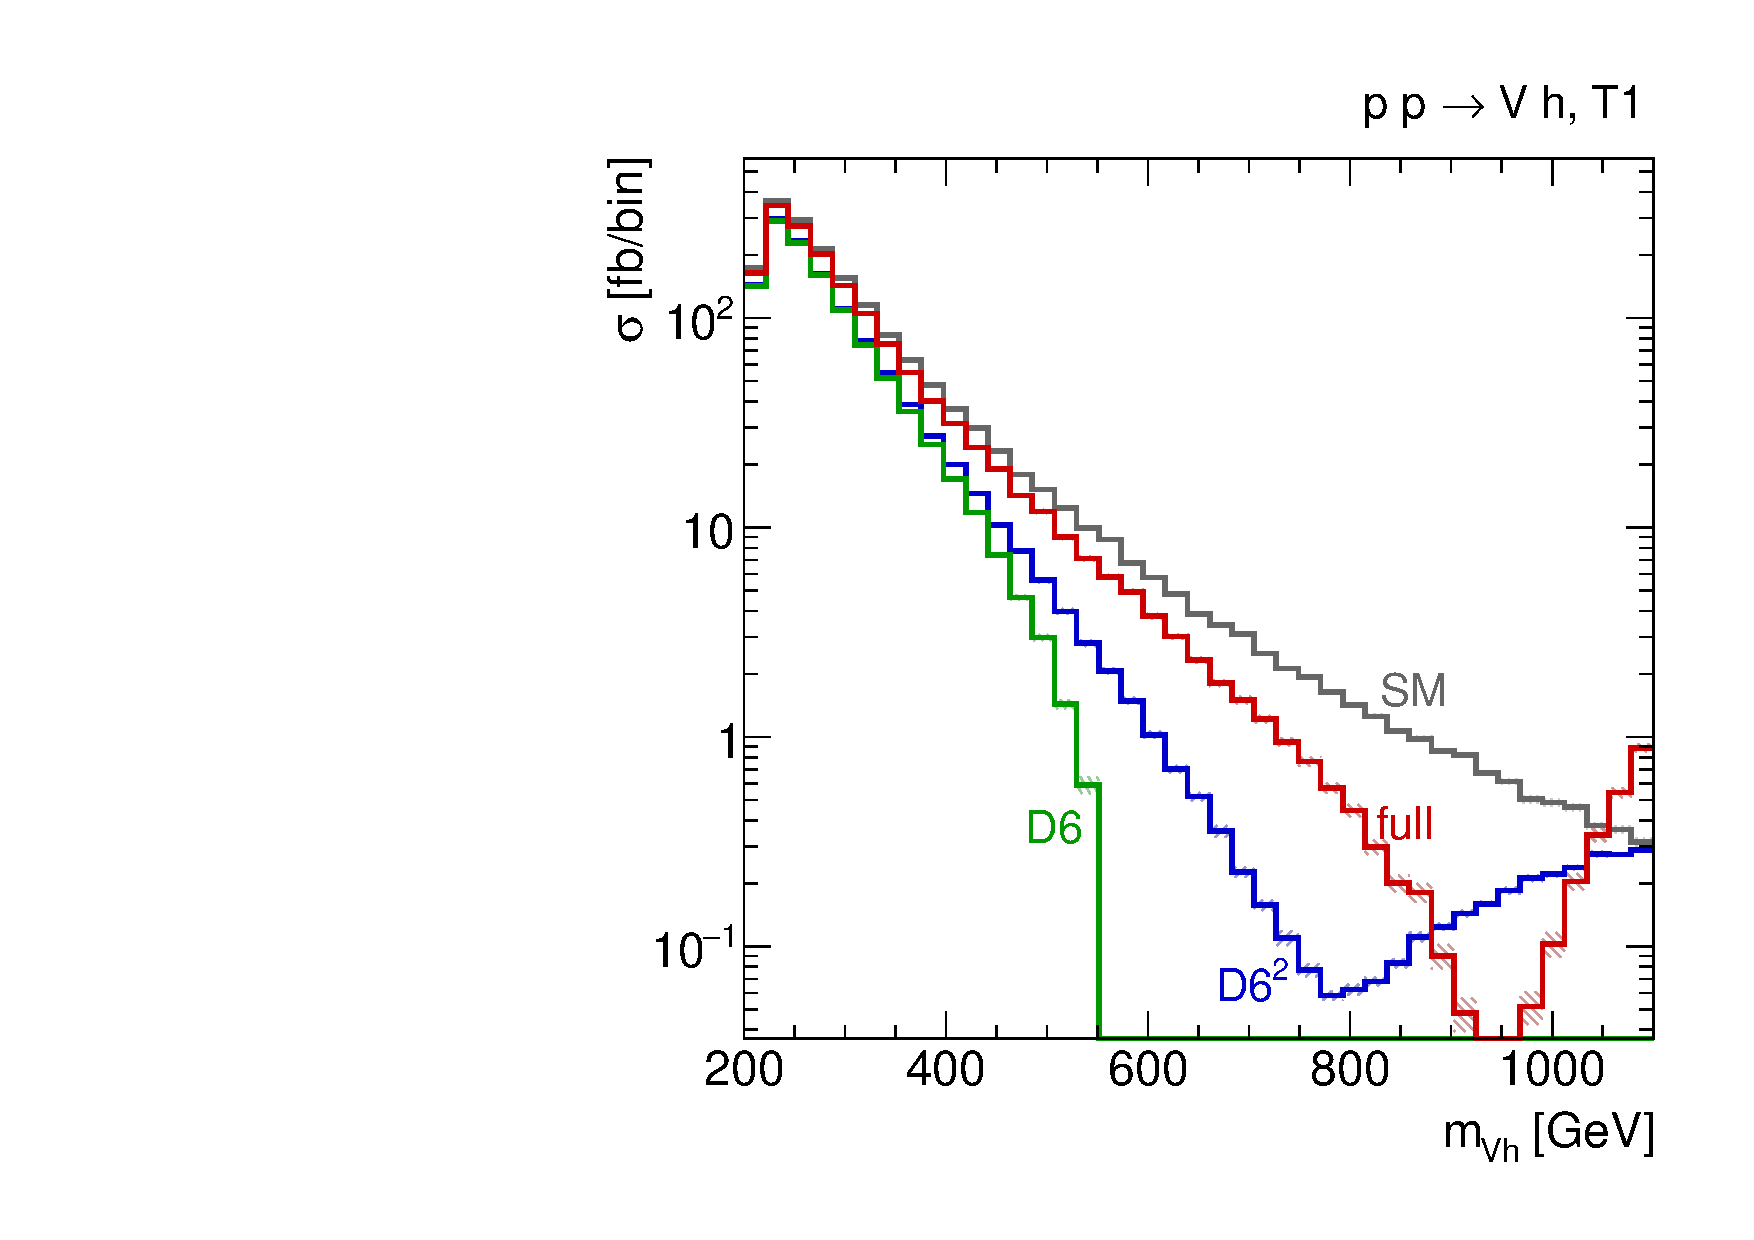
\includegraphics[width=0.43\textwidth]{fig/validity/VH_T1_mVH.pdf}
  \hspace*{0.05\textwidth}
  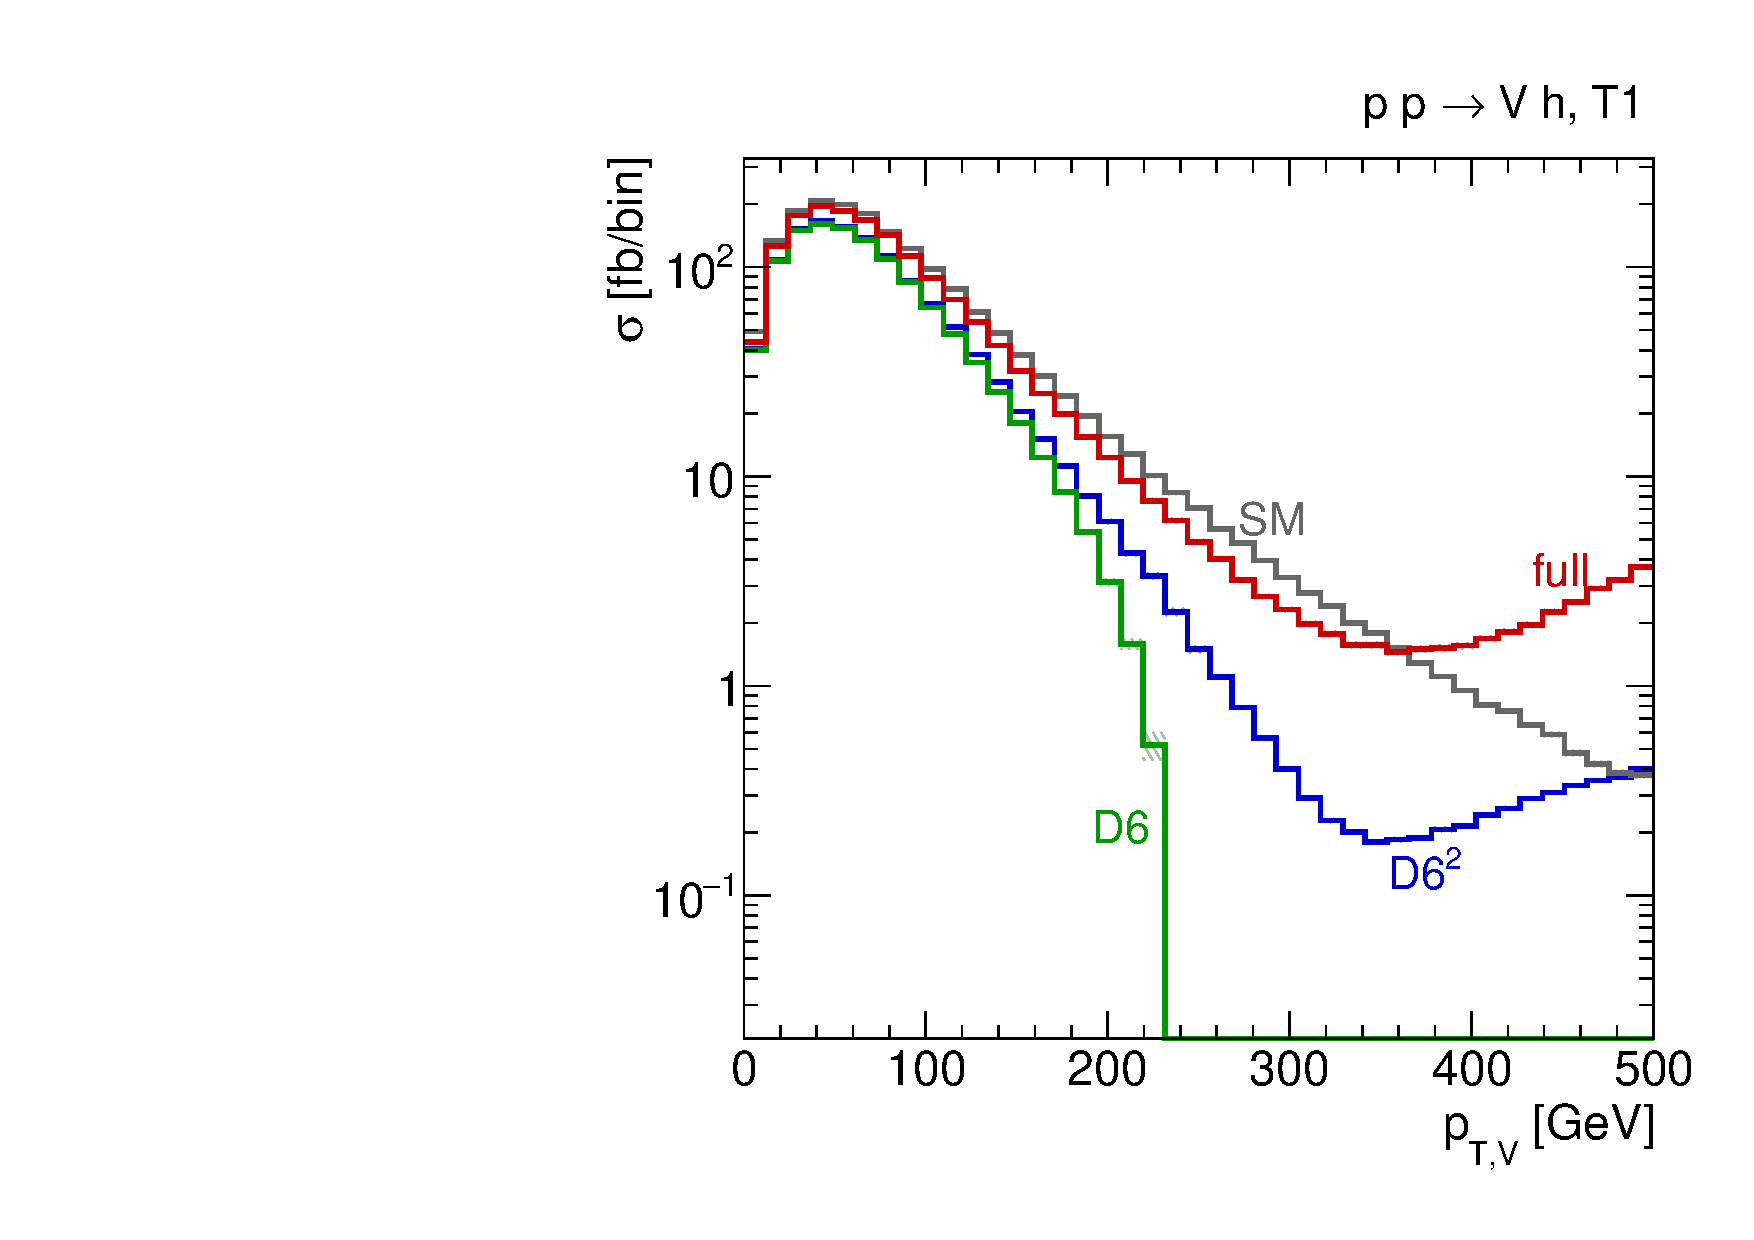
\includegraphics[width=0.43\textwidth]{fig/validity/VH_T1_Vpt.pdf} \\
  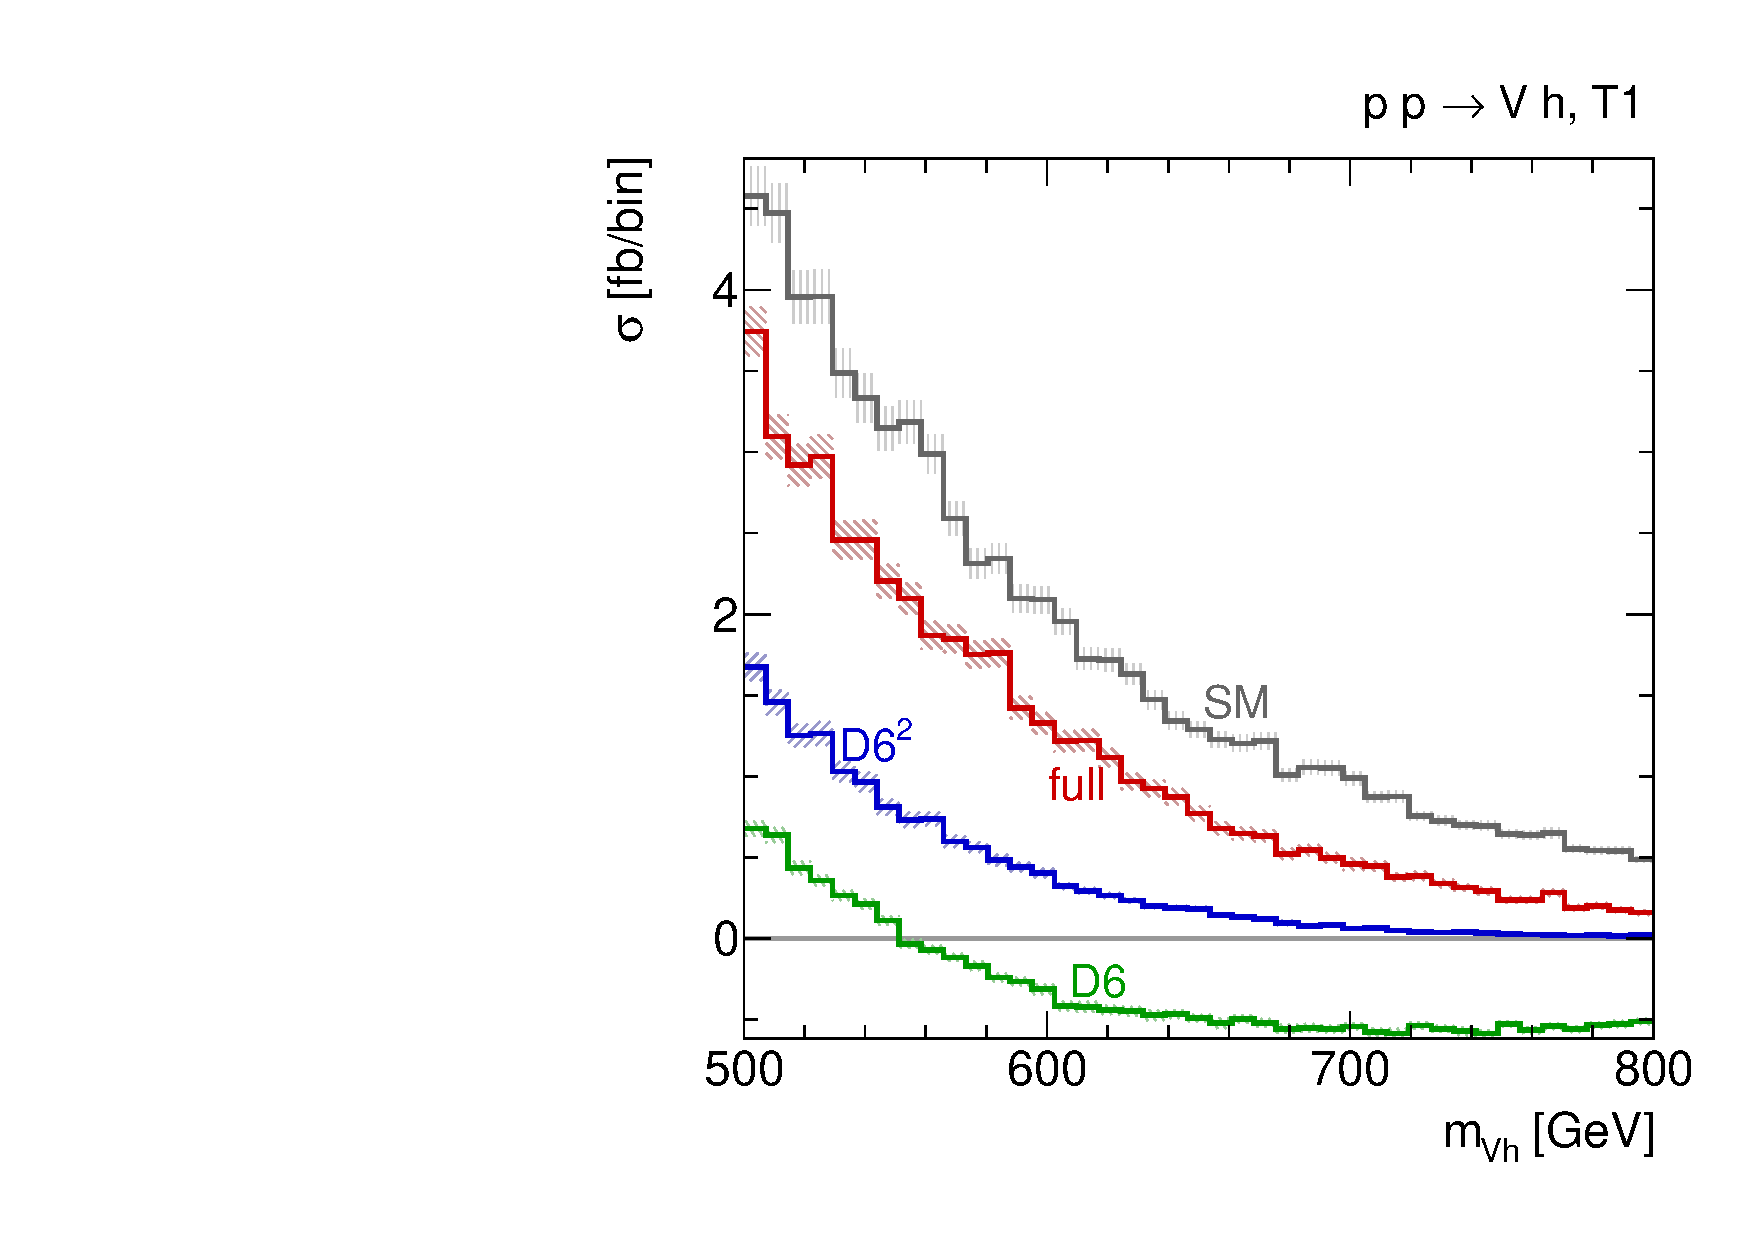
\includegraphics[width=0.43\textwidth]{fig/validity/VH_T1_mVH_zoom.pdf} 
  \hspace*{0.05\textwidth}
  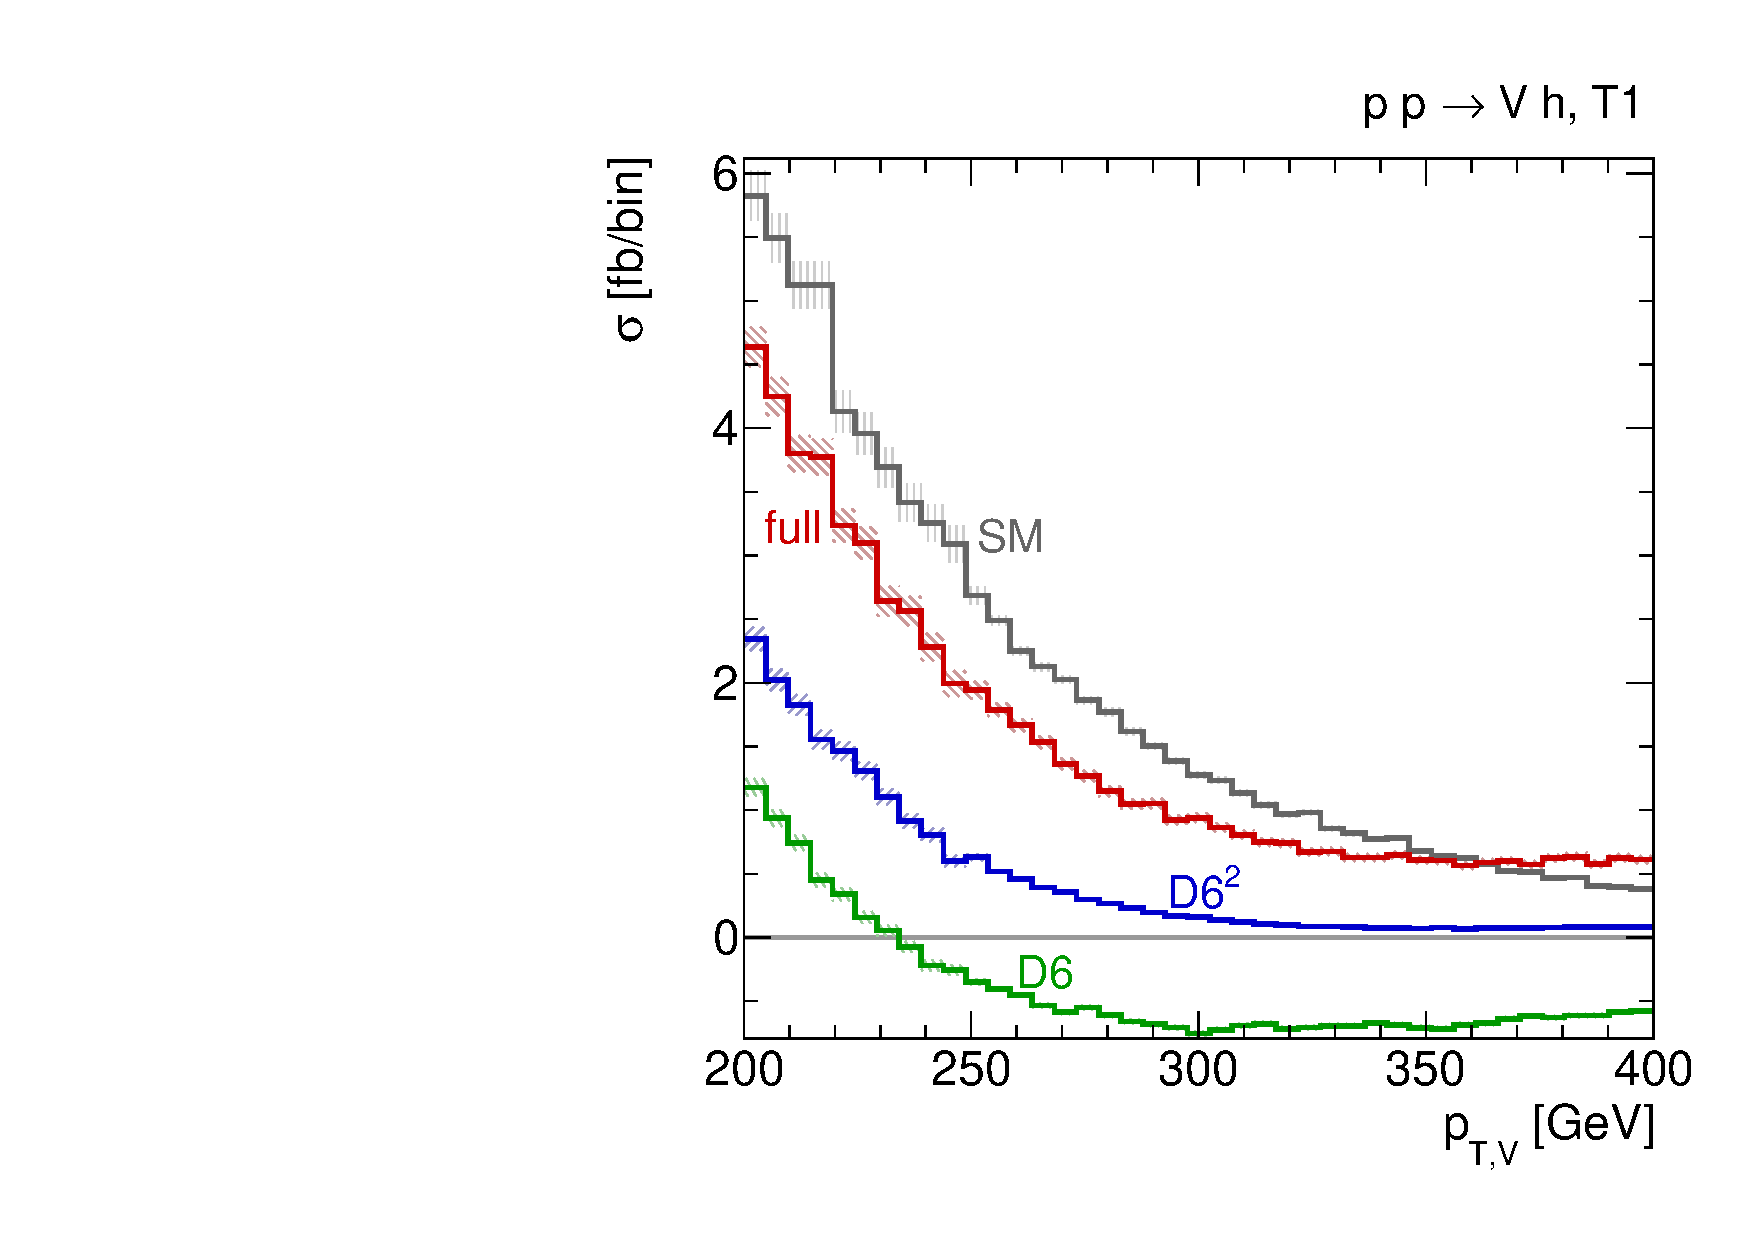
\includegraphics[width=0.43\textwidth]{fig/validity/VH_T1_Vpt_zoom} \\
  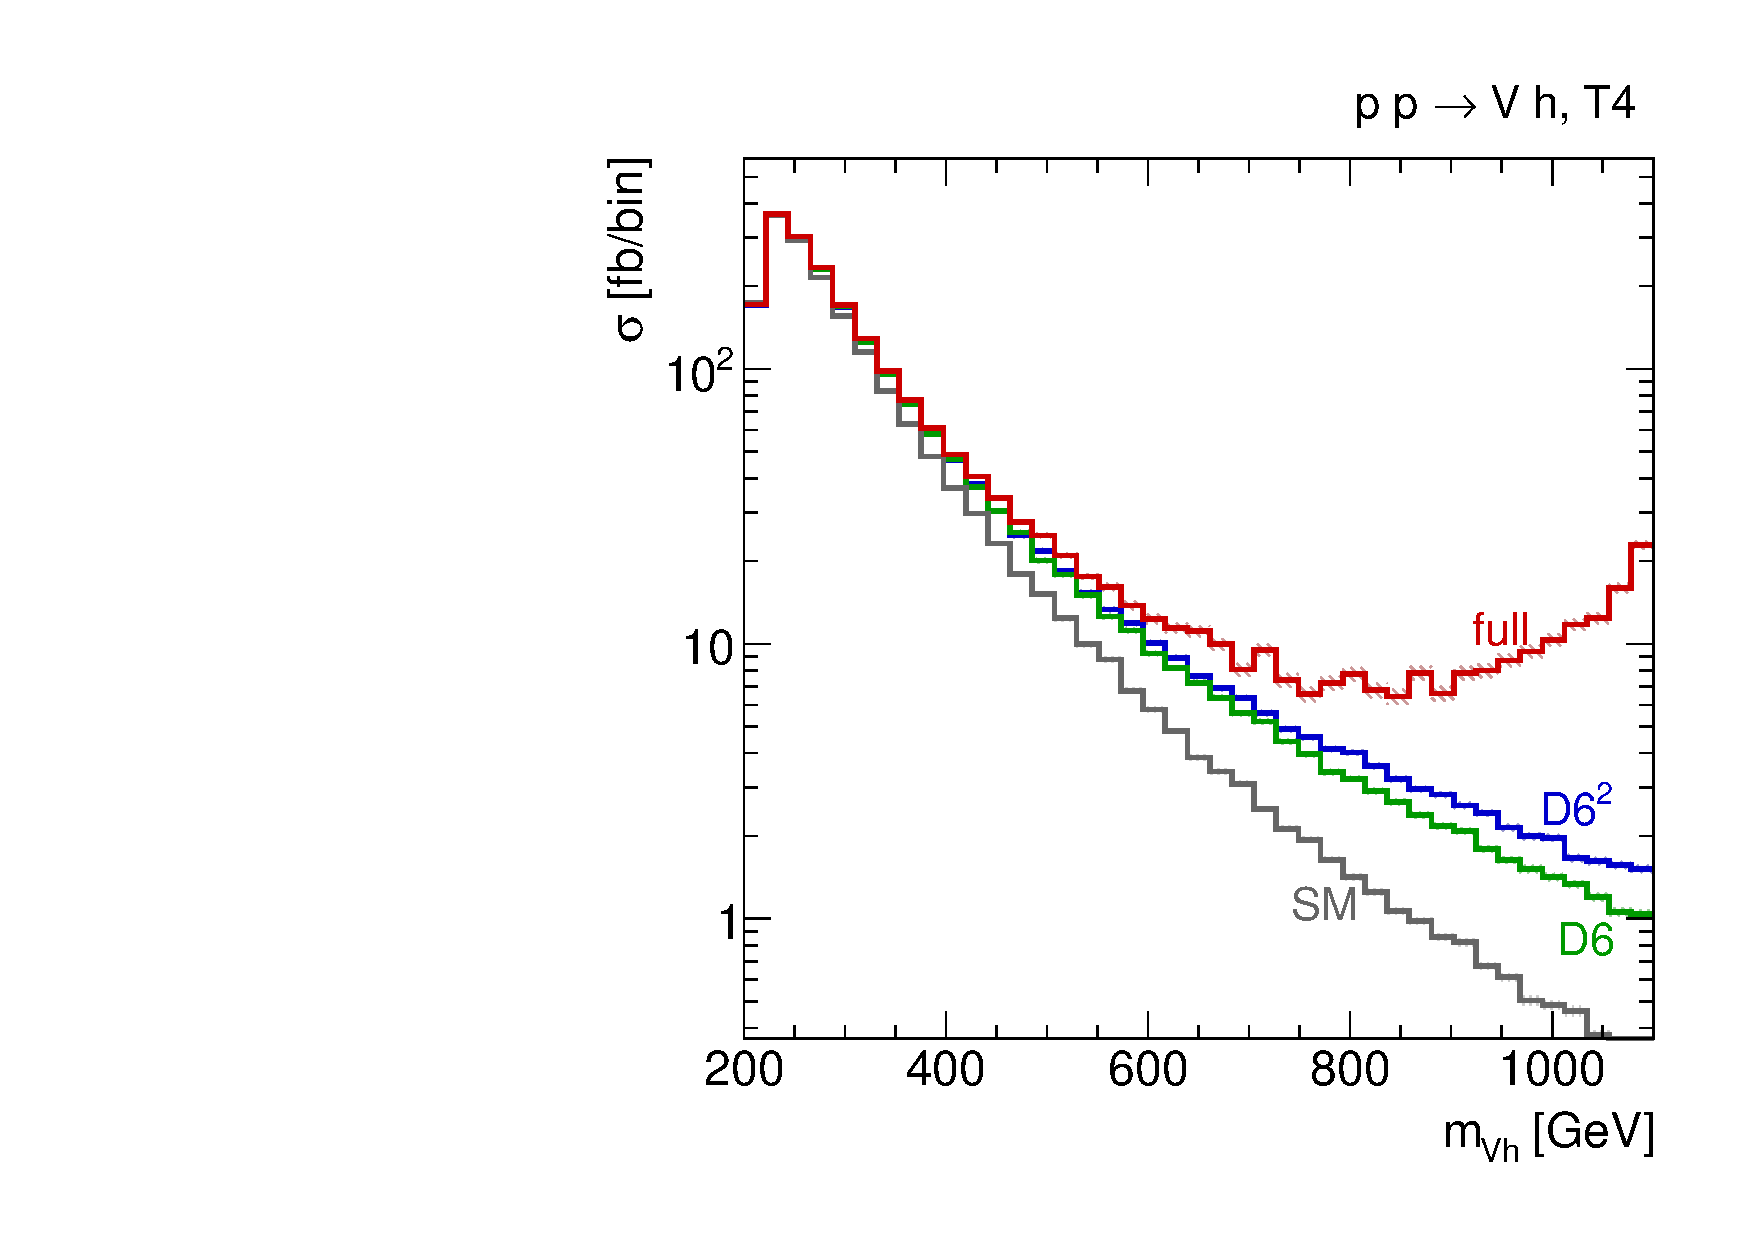
\includegraphics[width=0.43\textwidth]{fig/validity/VH_T4_mVH}
  \hspace*{0.05\textwidth}
  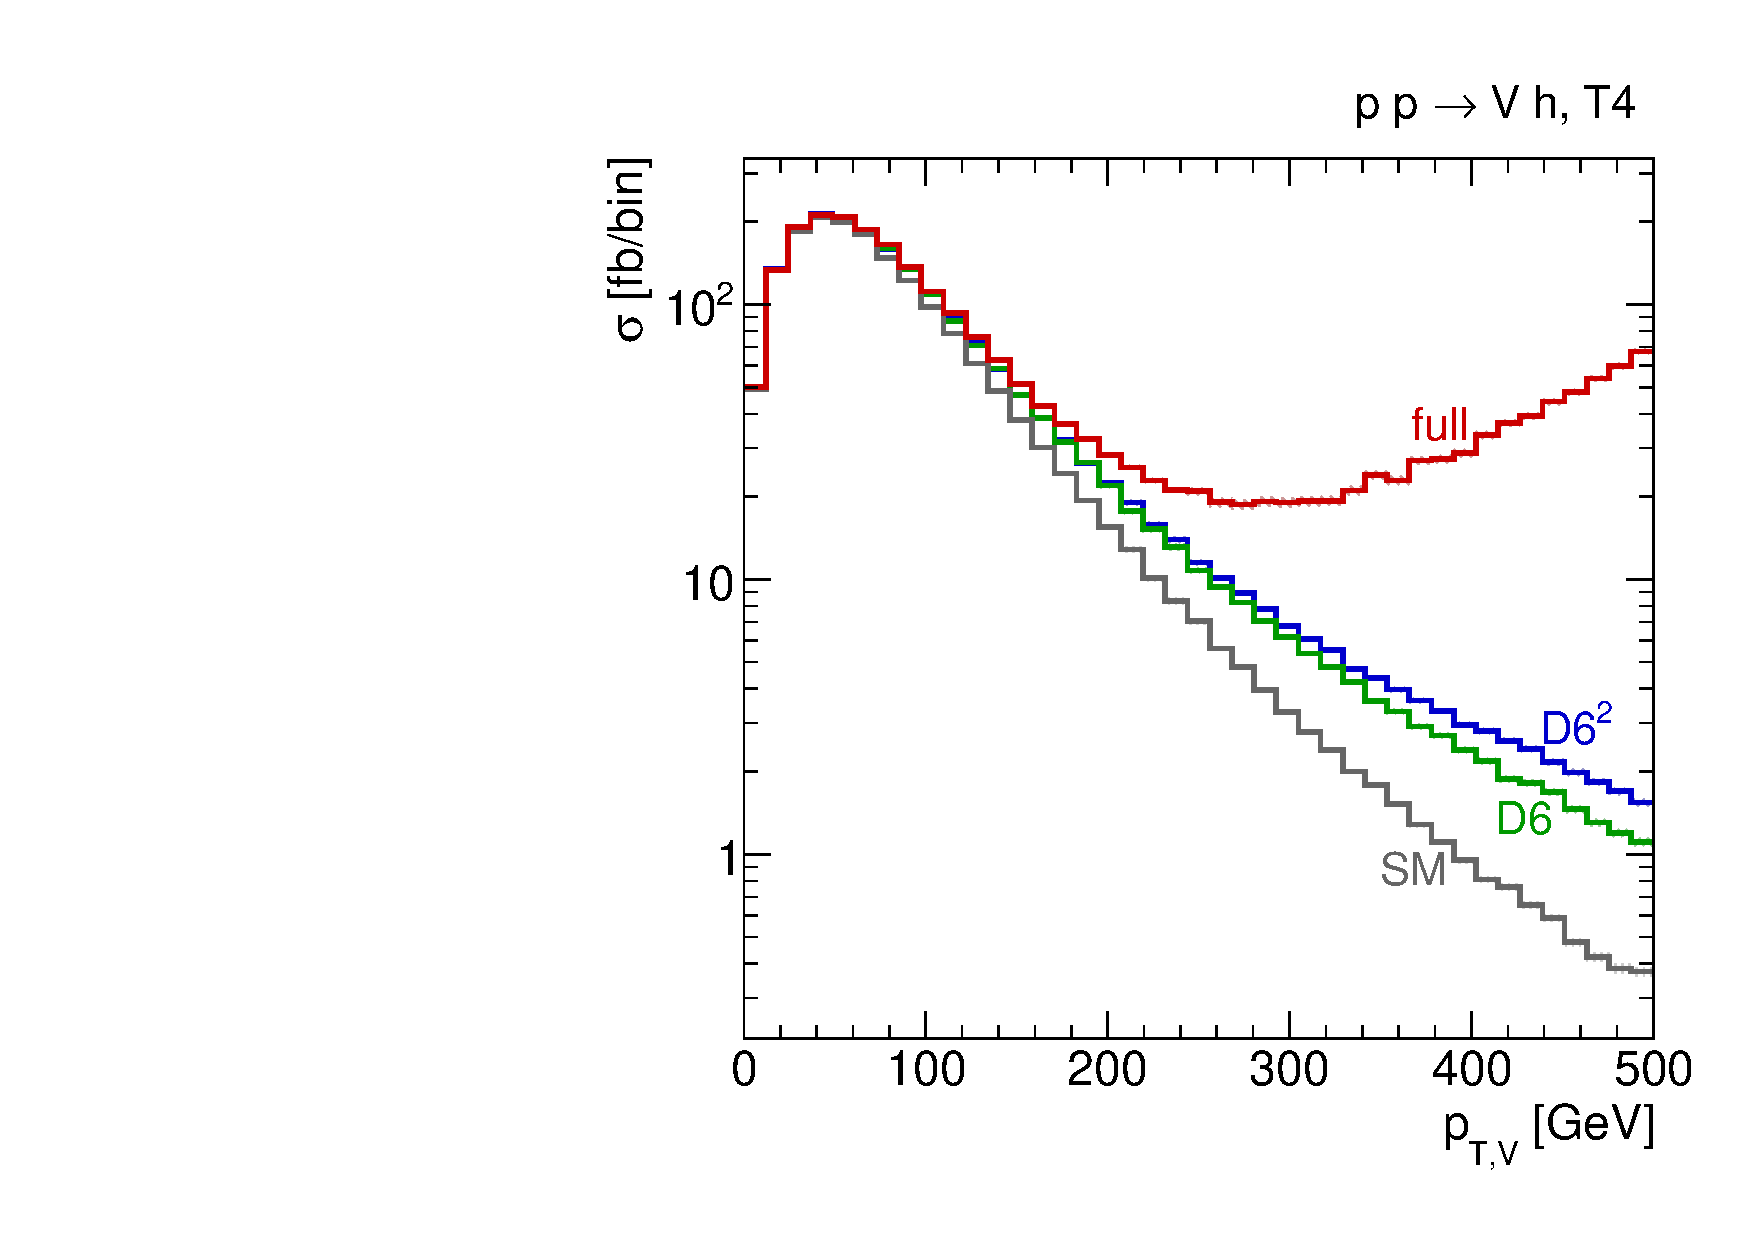
\includegraphics[width=0.43\textwidth]{fig/validity/VH_T4_Vpt}
  \caption{$Vh$ distributions with (``D6$^{2}$'') and without (``D6'')
    the dimension-6 squared
    term. The left panels show $m_{VH}$, the right panels
    $p_{T,V}$. The central panels show the region where leaving out
    the squared dimension-6 terms leads to a negative cross section.}
  \label{fig:validity_squared_VH}
\end{figure}
%------------------------------------------------------------


%%%%%%%%%%%%%%%%%%%%%%%%%%%%%%%%%%%%%%%%%%%%%%%%%%%%%%%%%%%%
\subsubsection*{WBF Higgs production}
%%%%%%%%%%%%%%%%%%%%%%%%%%%%%%%%%%%%%%%%%%%%%%%%%%%%%%%%%%%%

Weak-boson-fusion Higgs production is a $2 \to 3$ process with two
$t$-channel gauge bosons carrying the momentum to the Higgs vertex.
The relevant kinematic variables are the two virtualities of the weak
bosons. Following many studies in the framework of the effective $W$
approximation~\cite{effective_w,polarized_ww} it is straightforward to
link them to the $p_T$ of the tagging jets, which even for multiple
jet radiation can be linked to the transverse momentum of the
Higgs~\cite{Buschmann:2014twa} (even though it is not clear if this
distribution is theoretically or experimentally favored).  Again, we
start with the parton-level signal process
%
\begin{align}
u d \to u' d' h
\label{eq:def_wbf}
\end{align}
%
with only one minimal cut $p_{T,j} > 20$~GeV for the two tagging jets.  We
show the results for the now constructively interfering benchmark
point T1 and the now destructively interfering benchmark point T4 in
Fig.~\ref{fig:validity_squared_WBF}. Negative event rates for T4 appear around
%
\begin{align}
p_{T,j_1} > 600~\gev \approx \frac{m_\xi^\text{(T4)}}{2} \; , 
\label{eq:breakdown_wbf}
\end{align}
%
forcing us to either disregard the corresponding model hypothesis or
to add the dimension-6 squared term.  For the less critical point T1
the agreement between the vector triplet model and its dimension-6
approximation including the squared terms extends well into the range
where deviations from the Standard Model become visible.

%------------------------------------------------------------
\begin{figure}
  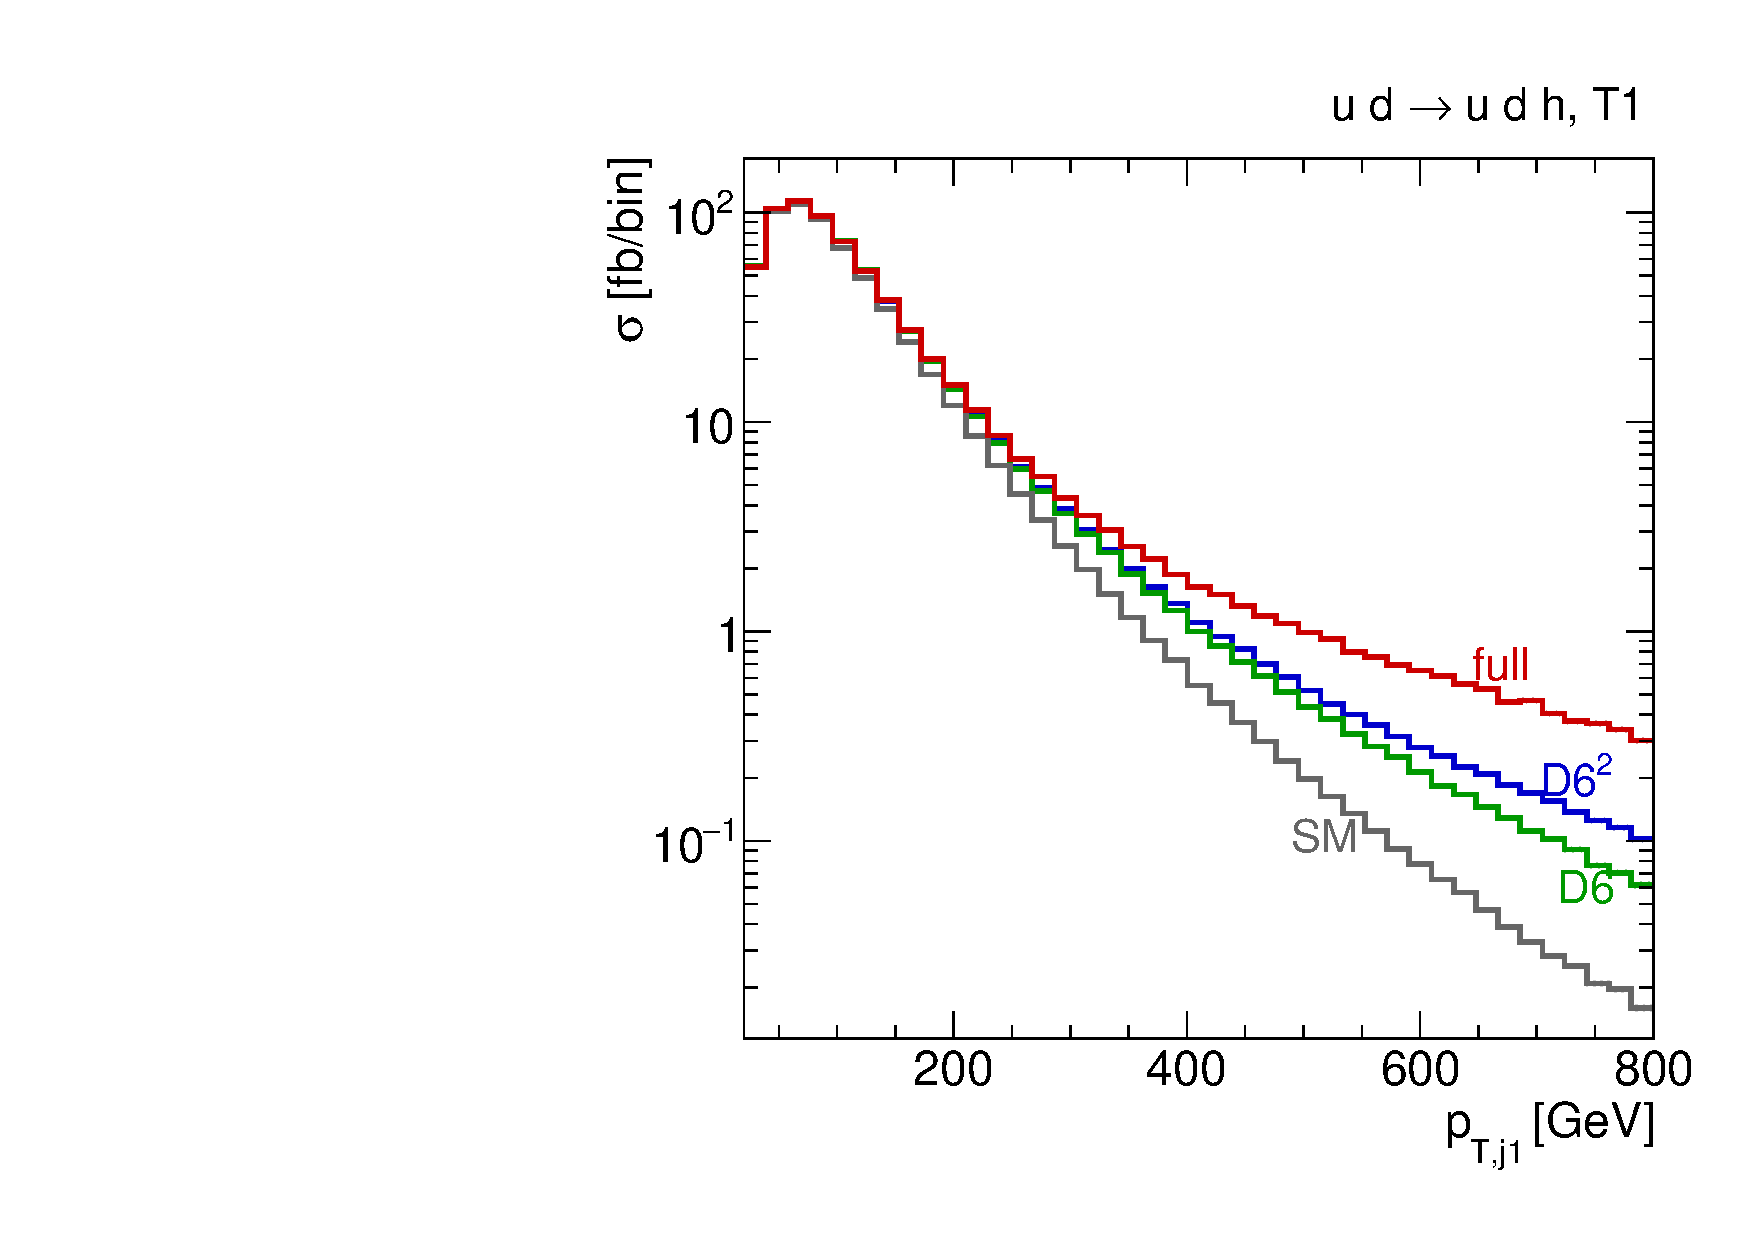
\includegraphics[width=0.43\textwidth]{fig/validity/WBF_T1_j1pt.pdf} 
  \hspace*{0.05\textwidth}
  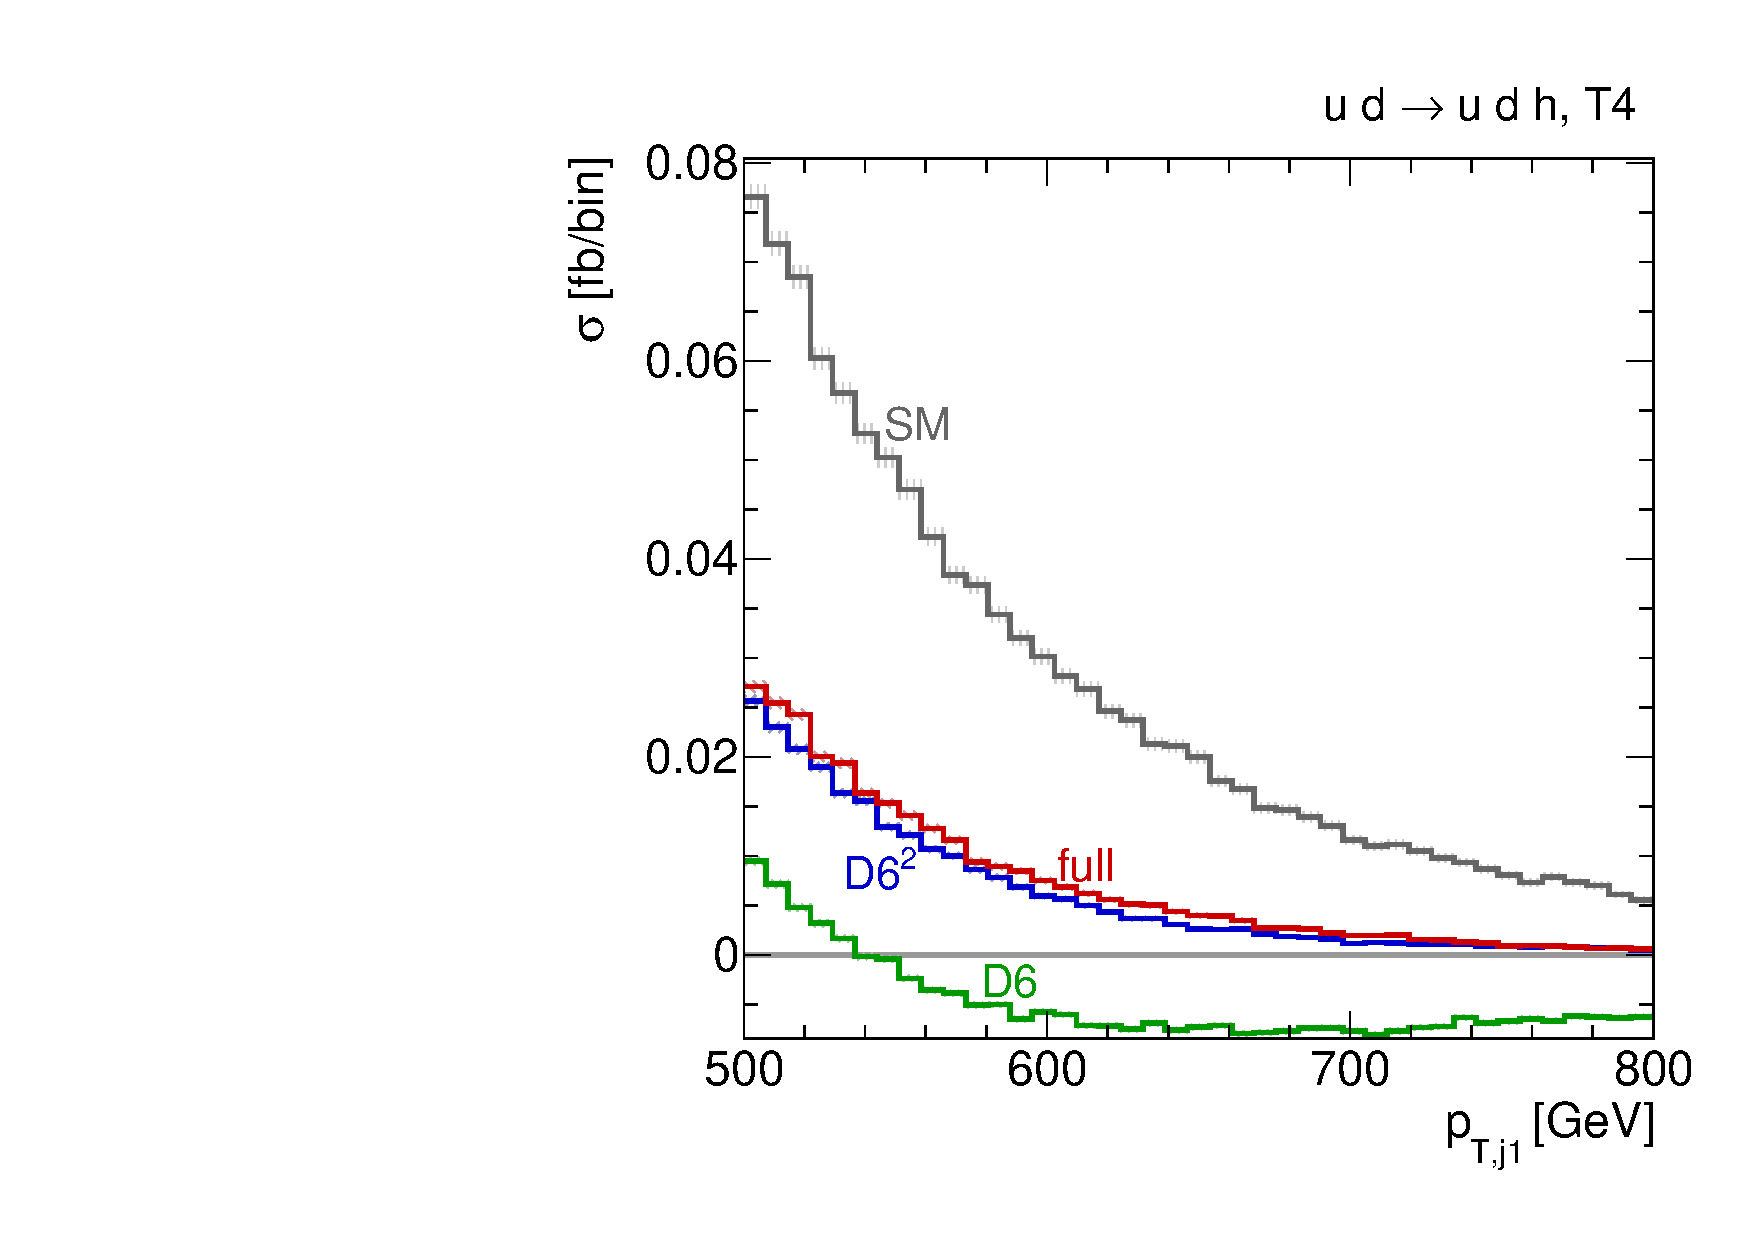
\includegraphics[width=0.43\textwidth]{fig/validity/WBF_T4_j1pt_zoom.pdf}\\
  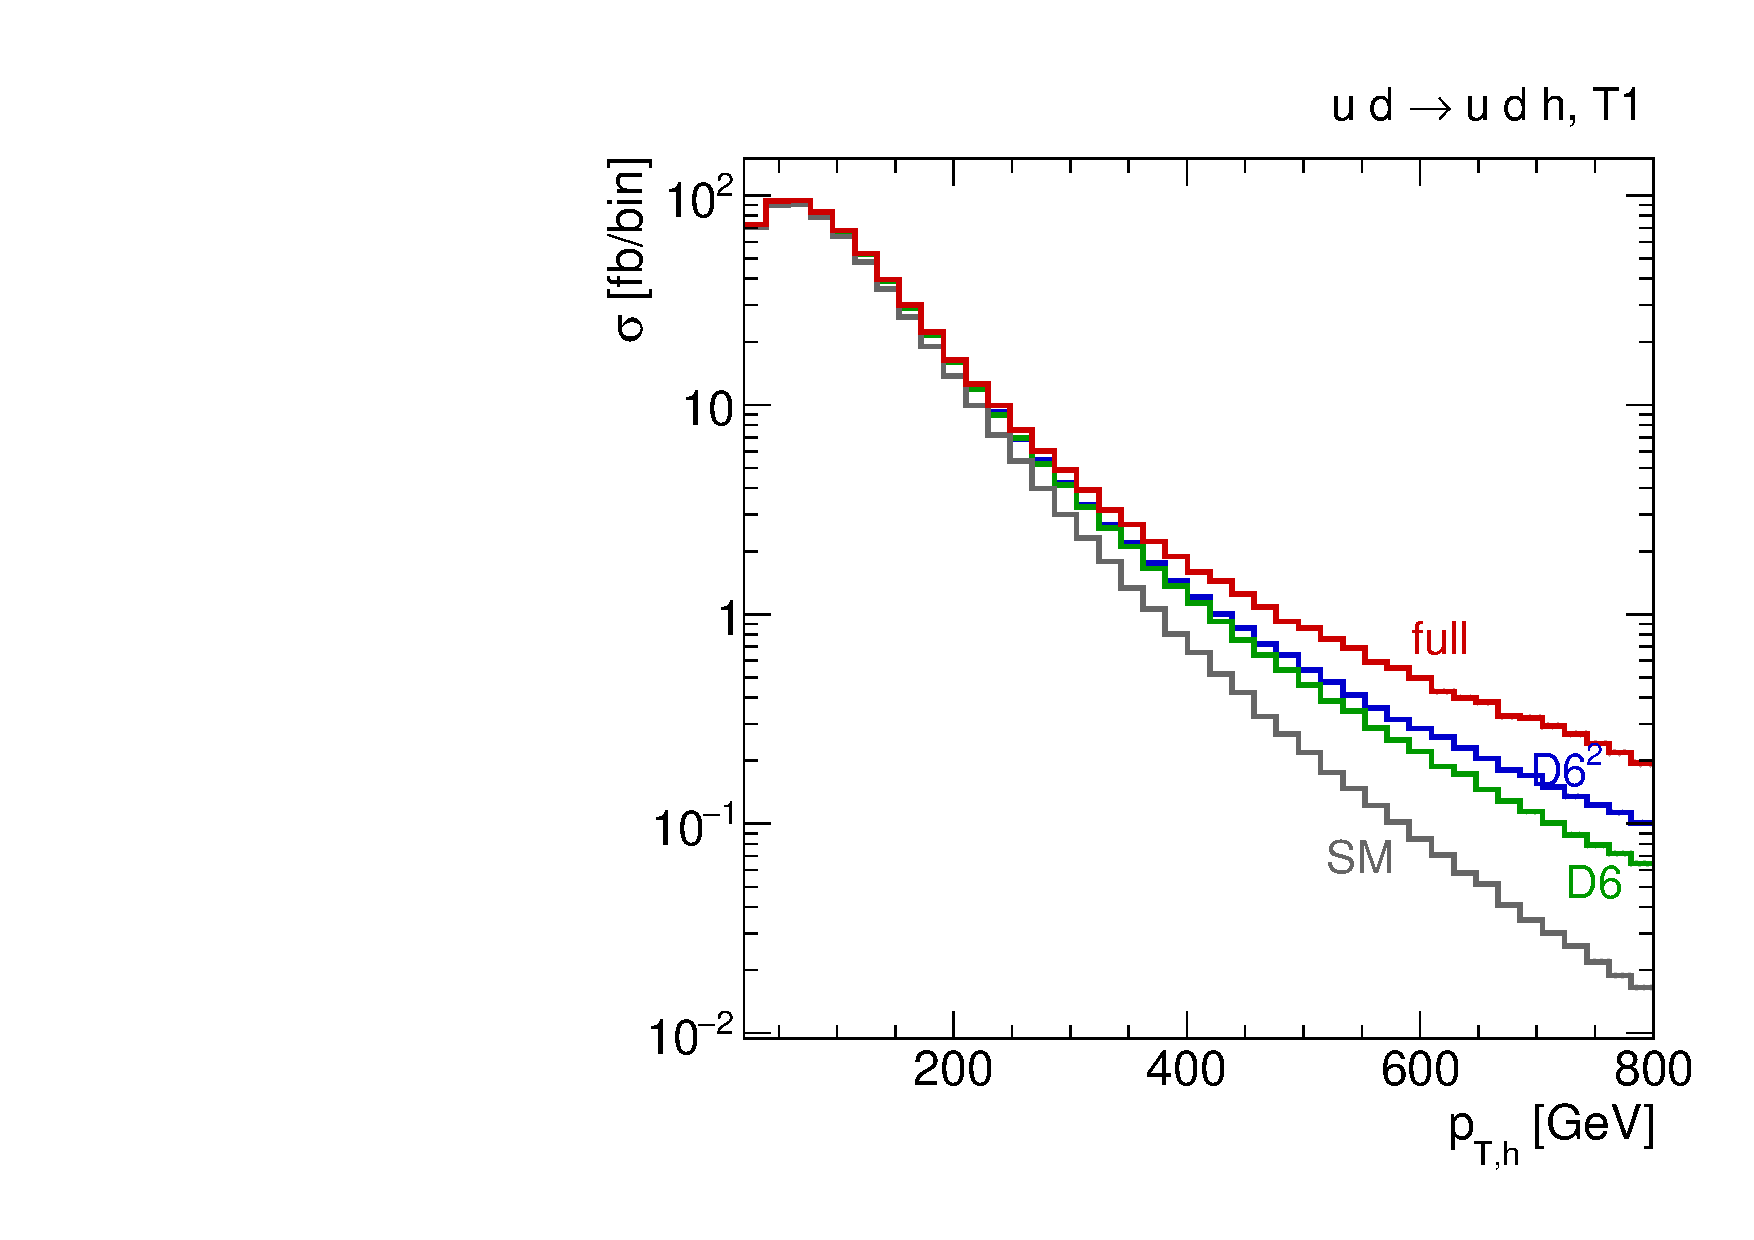
\includegraphics[width=0.43\textwidth]{fig/validity/WBF_T1_Hpt.pdf} 
  \hspace*{0.05\textwidth}
  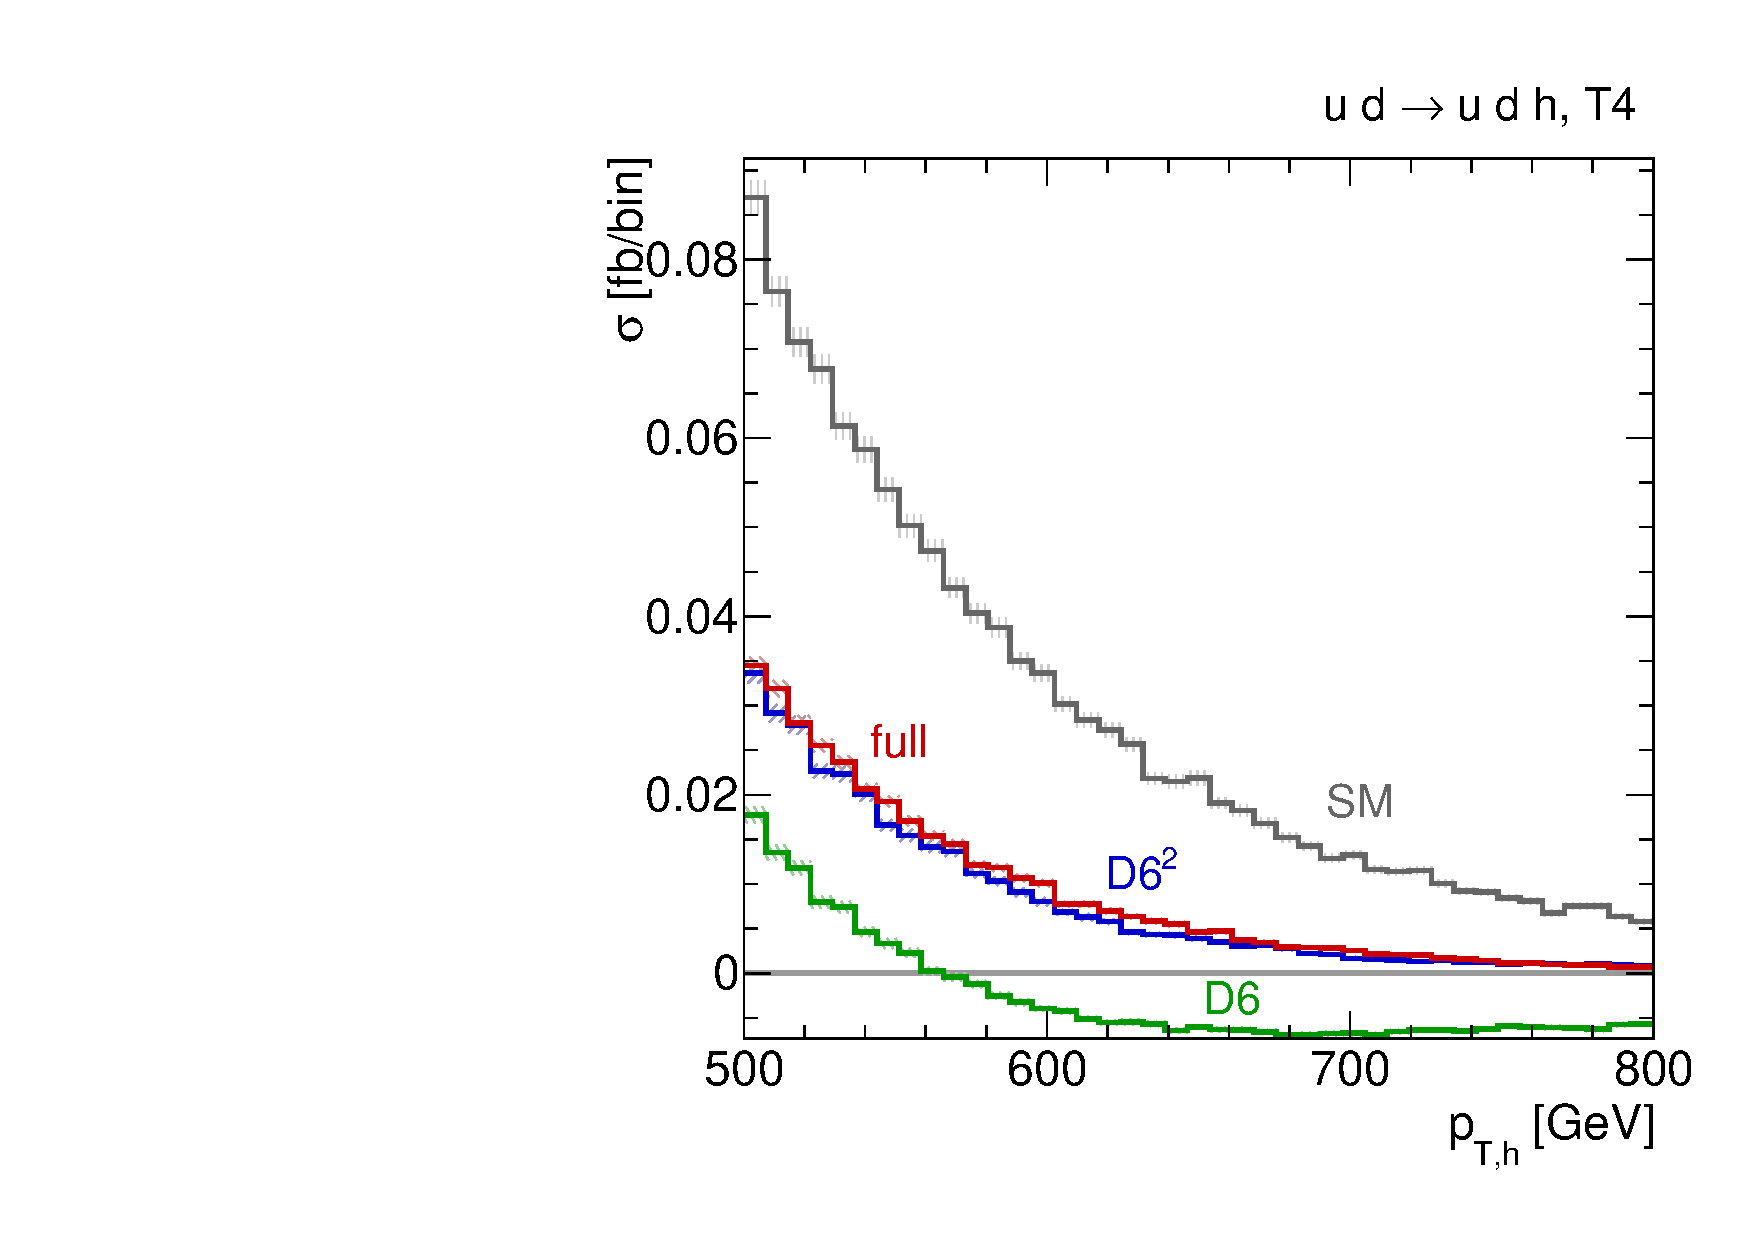
\includegraphics[width=0.43\textwidth]{fig/validity/WBF_T4_Hpt.pdf}\\
  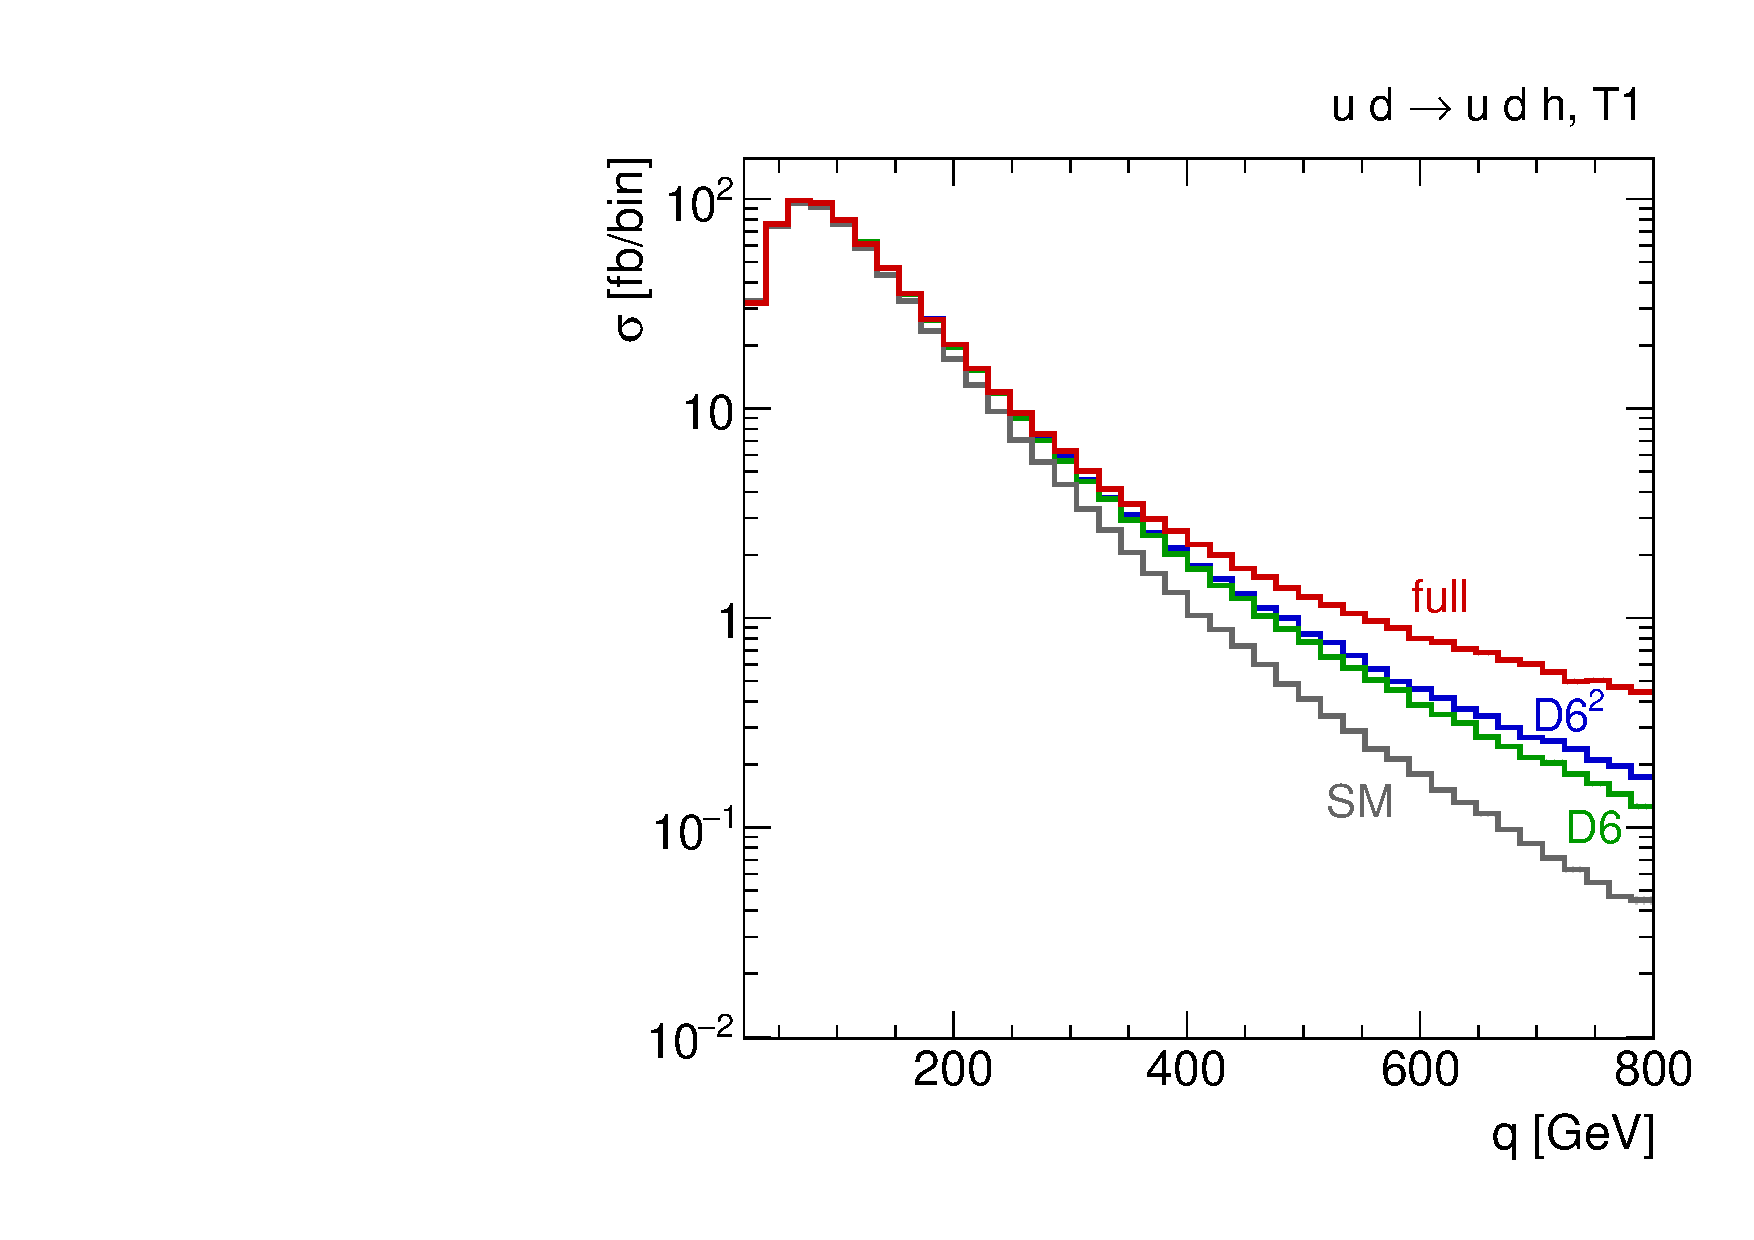
\includegraphics[width=0.43\textwidth]{fig/validity/WBF_T1_q.pdf} 
  \hspace*{0.05\textwidth}
  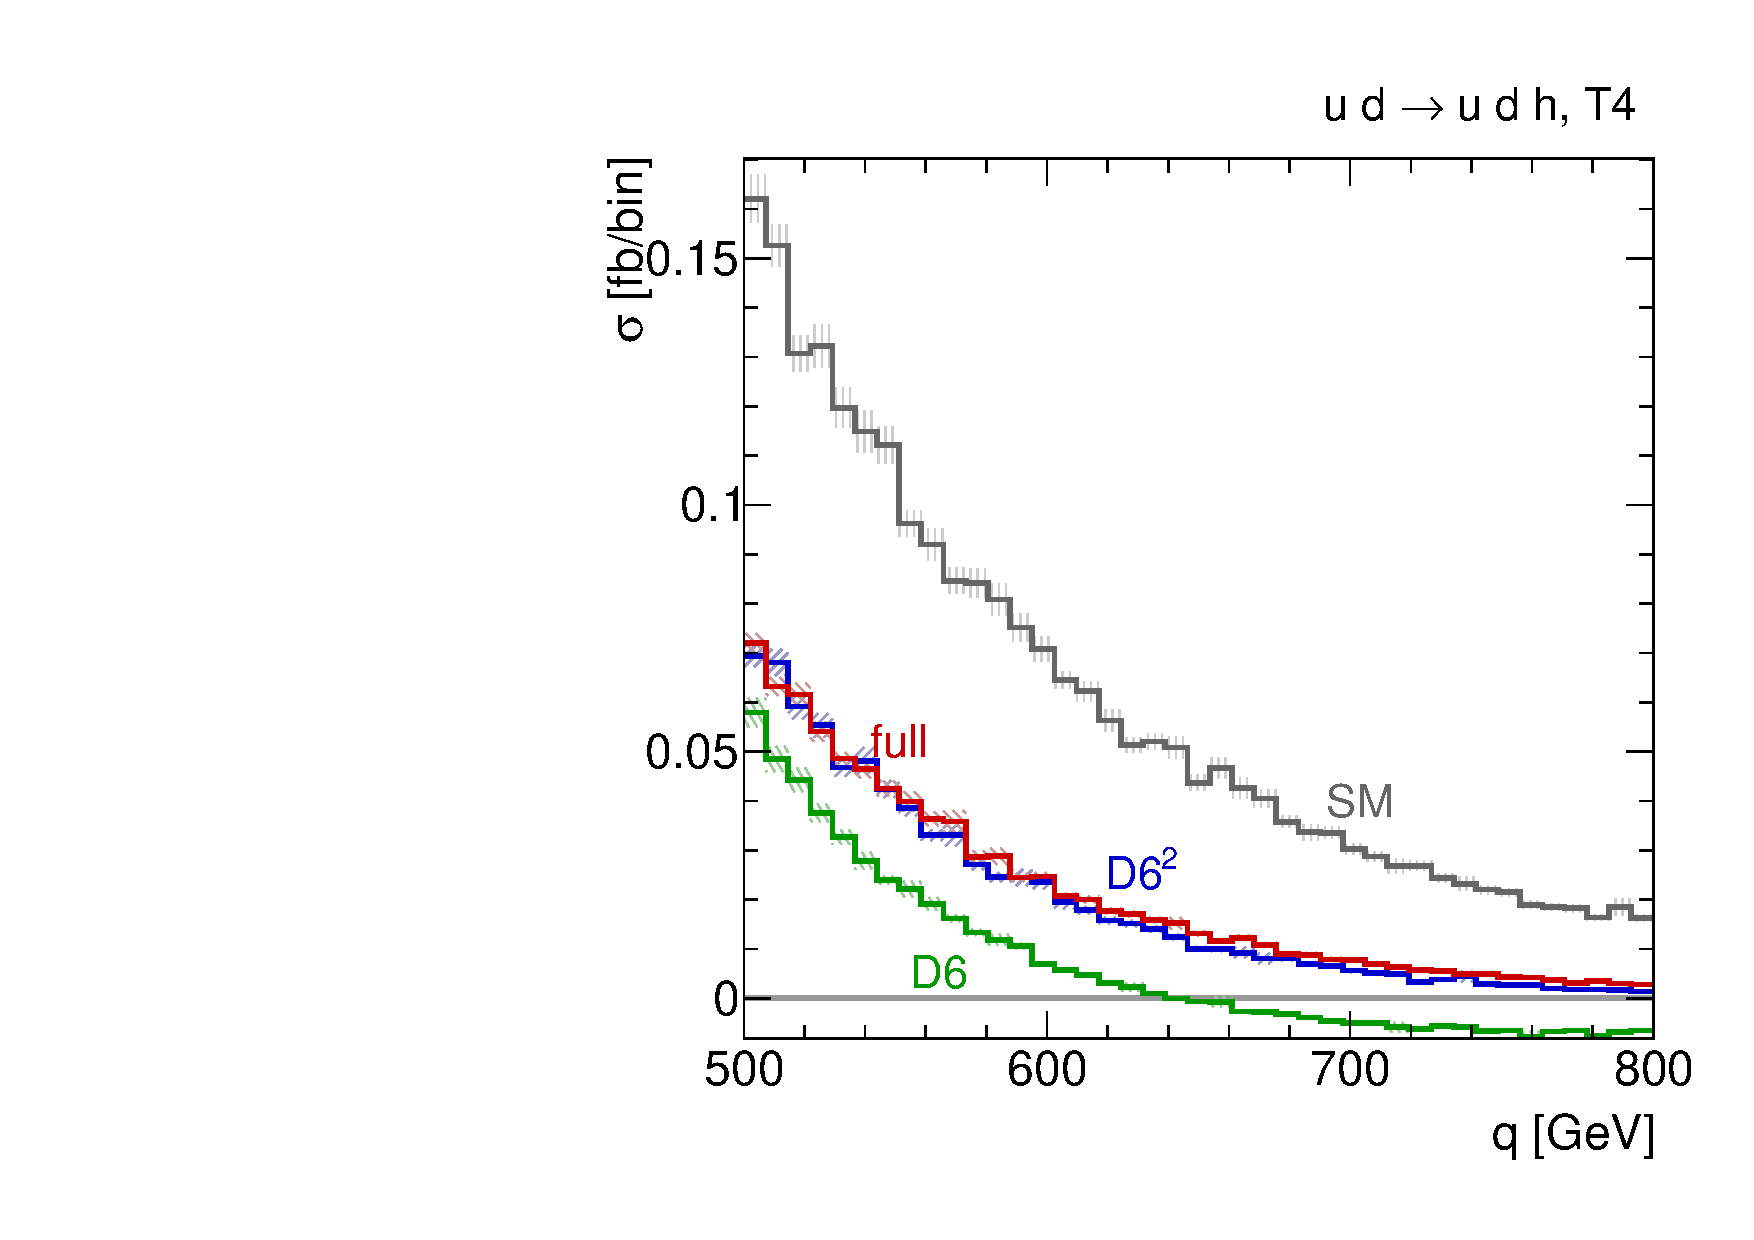
\includegraphics[width=0.43\textwidth]{fig/validity/WBF_T4_q.pdf}
  \caption{WBF distributions with (``D6$^{2}$'') and without (``D6'') the
    dimension-6 squared term. From top to bottom: $p_{T,j1}$, $p_{T,h}$, and
    virtuality $q$ defined in Eq.\;\eqref{eq:virt}. The right panels show the region where
    leaving out the squared dimension-6 terms leads to a negative cross
    section.}
  \label{fig:validity_squared_WBF}
\end{figure}
%------------------------------------------------------------


%------------------------------------------------------------
\begin{figure}[t]
  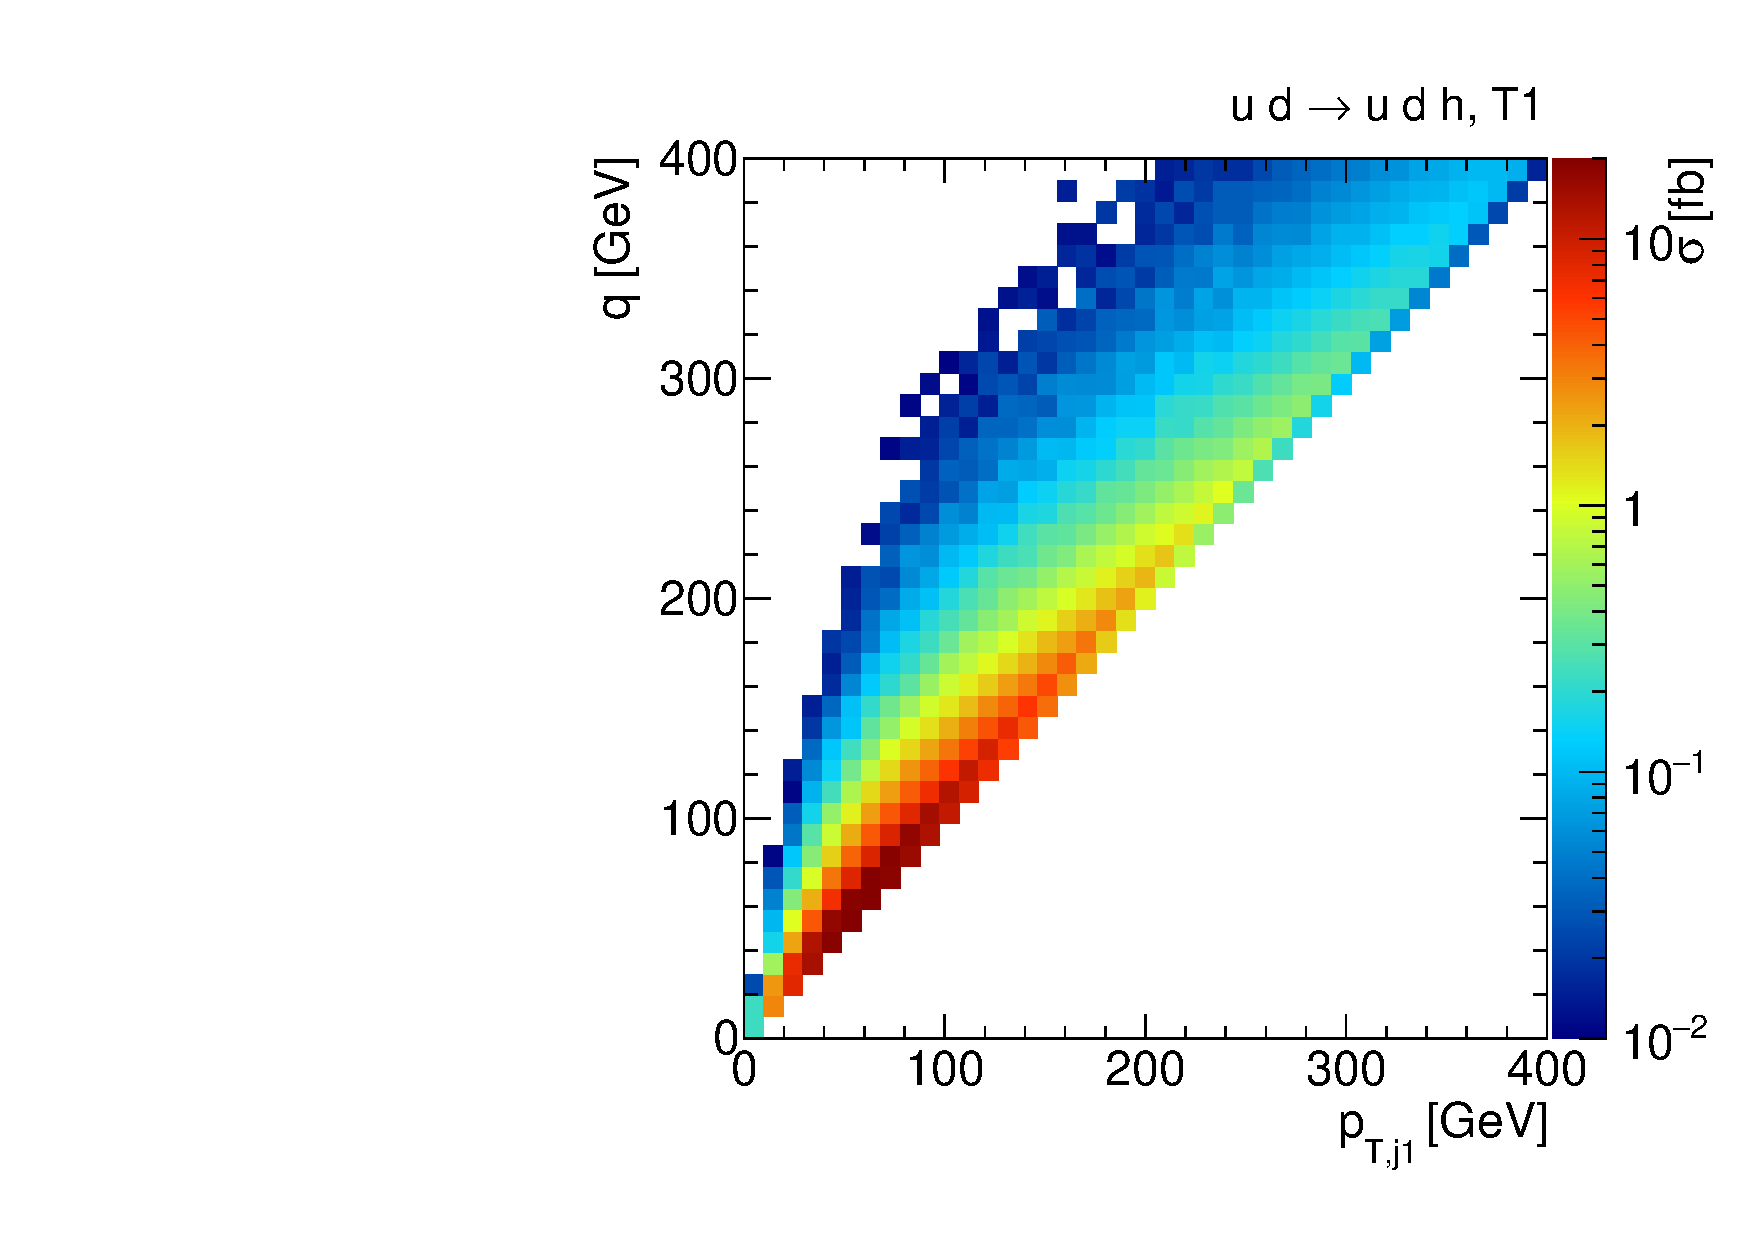
\includegraphics[width=0.43\textwidth]{fig/validity/WBF_correl_q_j1pt.pdf}
  \hspace*{0.05\textwidth}
  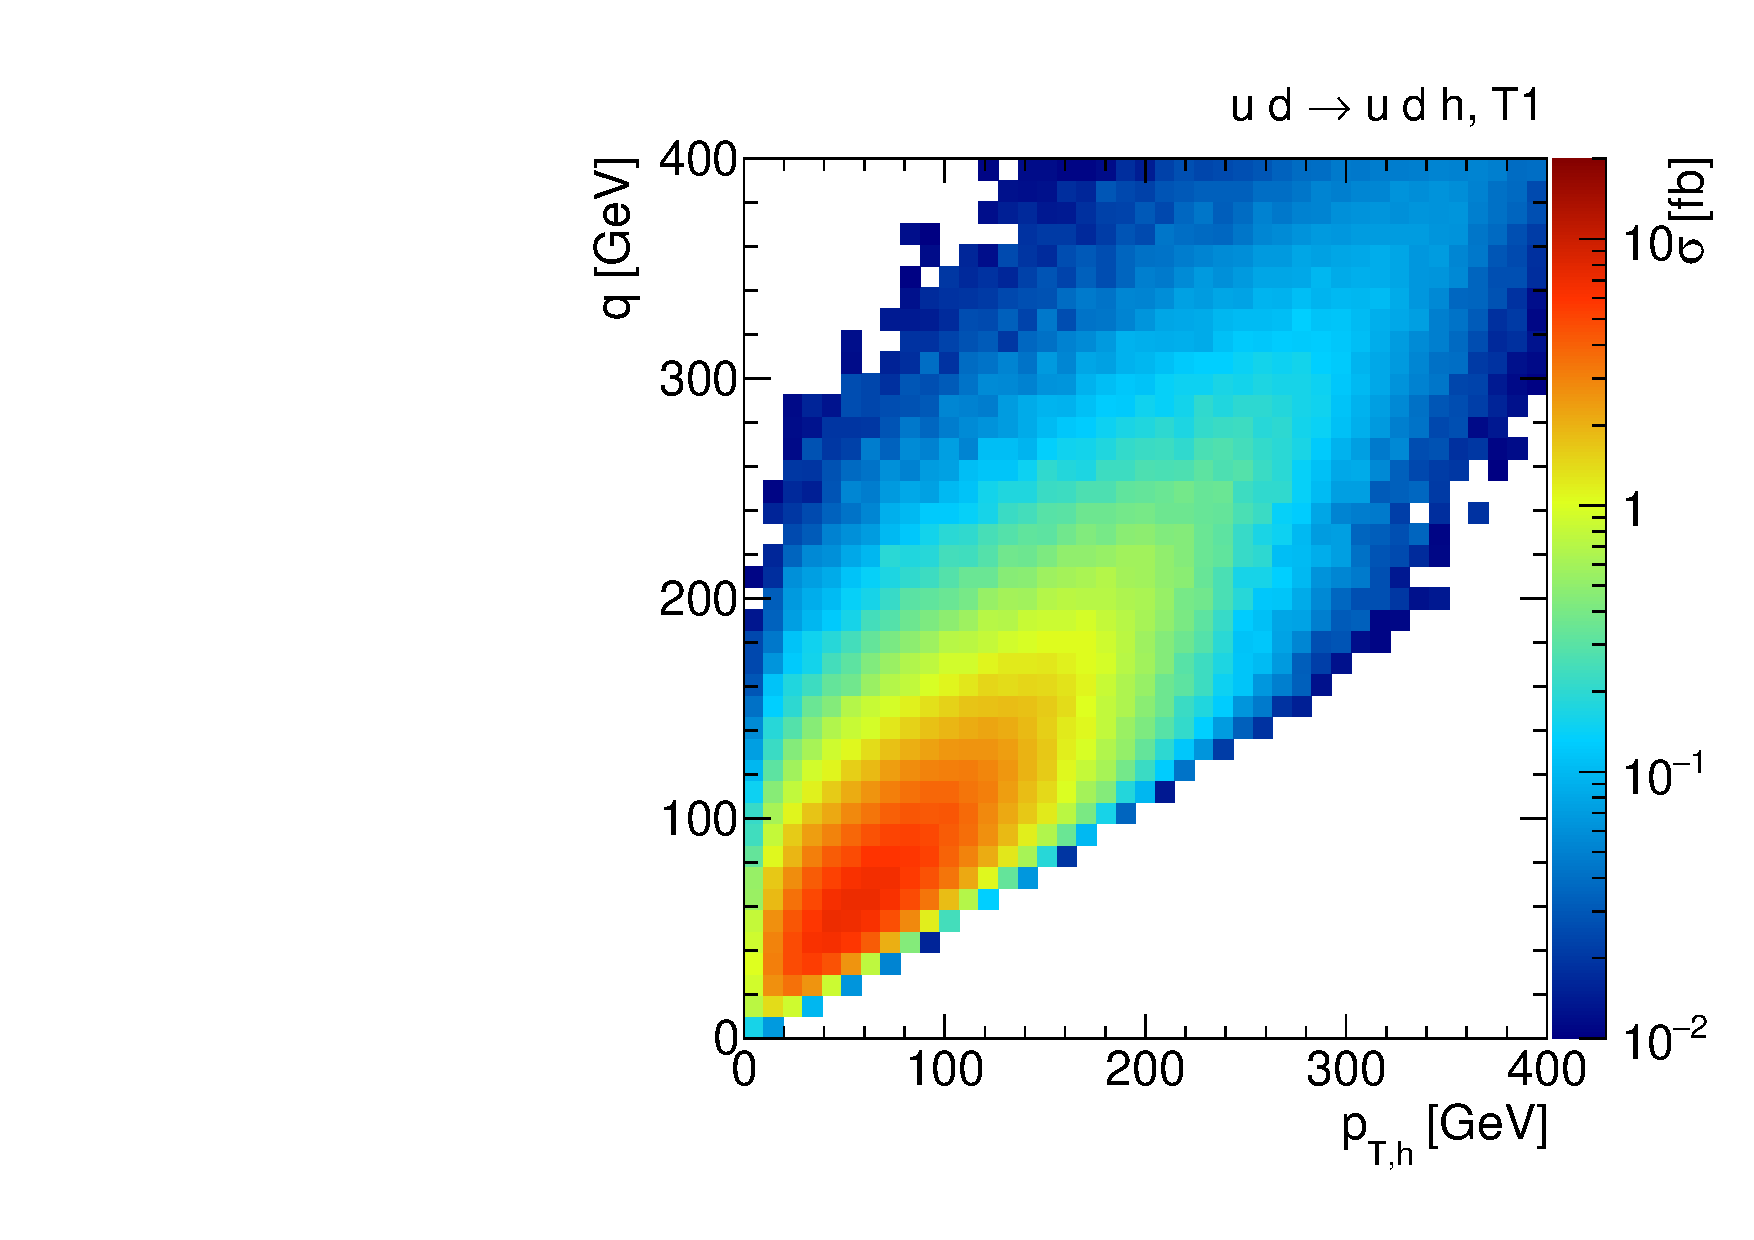
\includegraphics[width=0.43\textwidth]{fig/validity/WBF_correl_q_Hpt.pdf} 
  \caption{WBF correlations between the virtuality $q$ and
    $p_{T,j_1}$ (left) or $p_{T,h}$ (right).}
  \label{fig:validity_virt_corr}
\end{figure}
%------------------------------------------------------------

%------------------------------------------------------------
\begin{figure}[b!]
  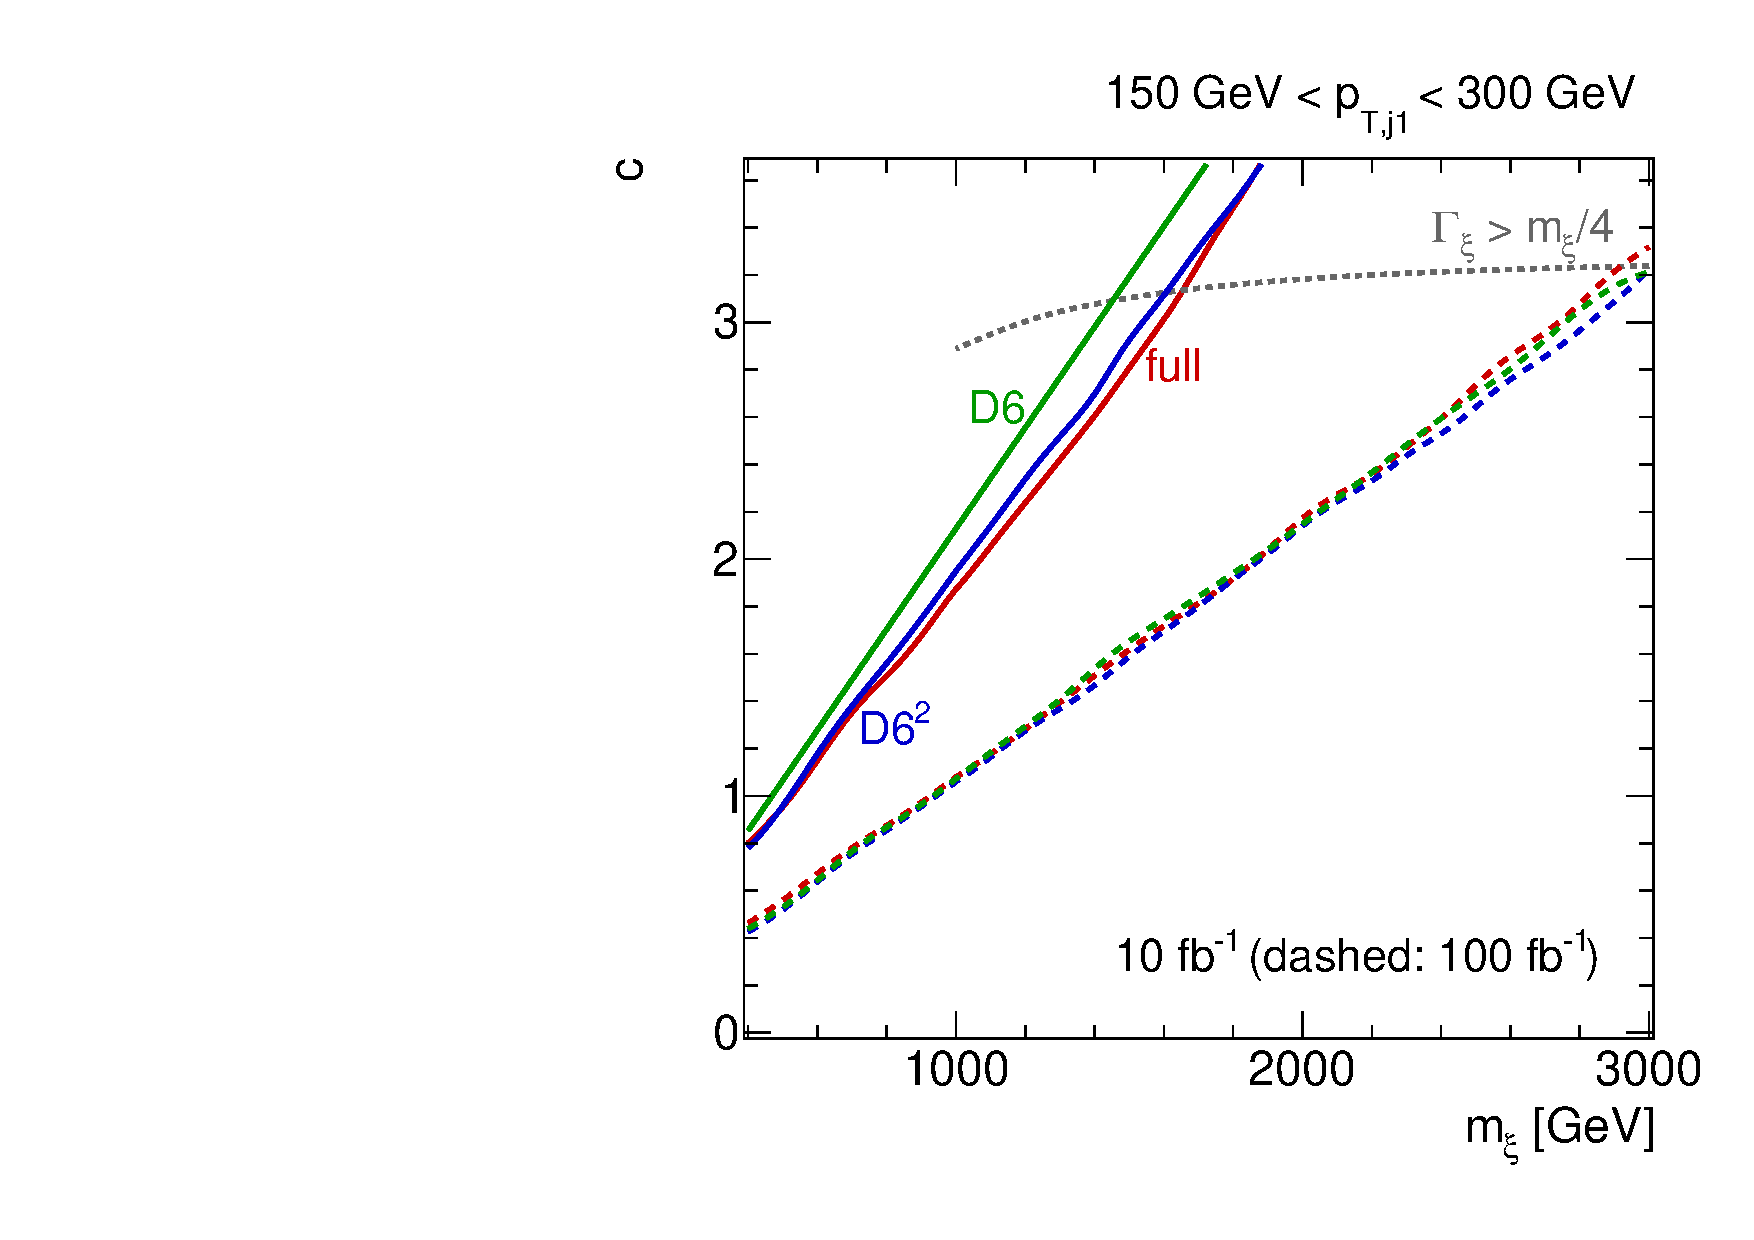
\includegraphics[width=0.43\textwidth]{fig/validity/WBF_limits_150.pdf}
  \hspace*{0.05\textwidth}
  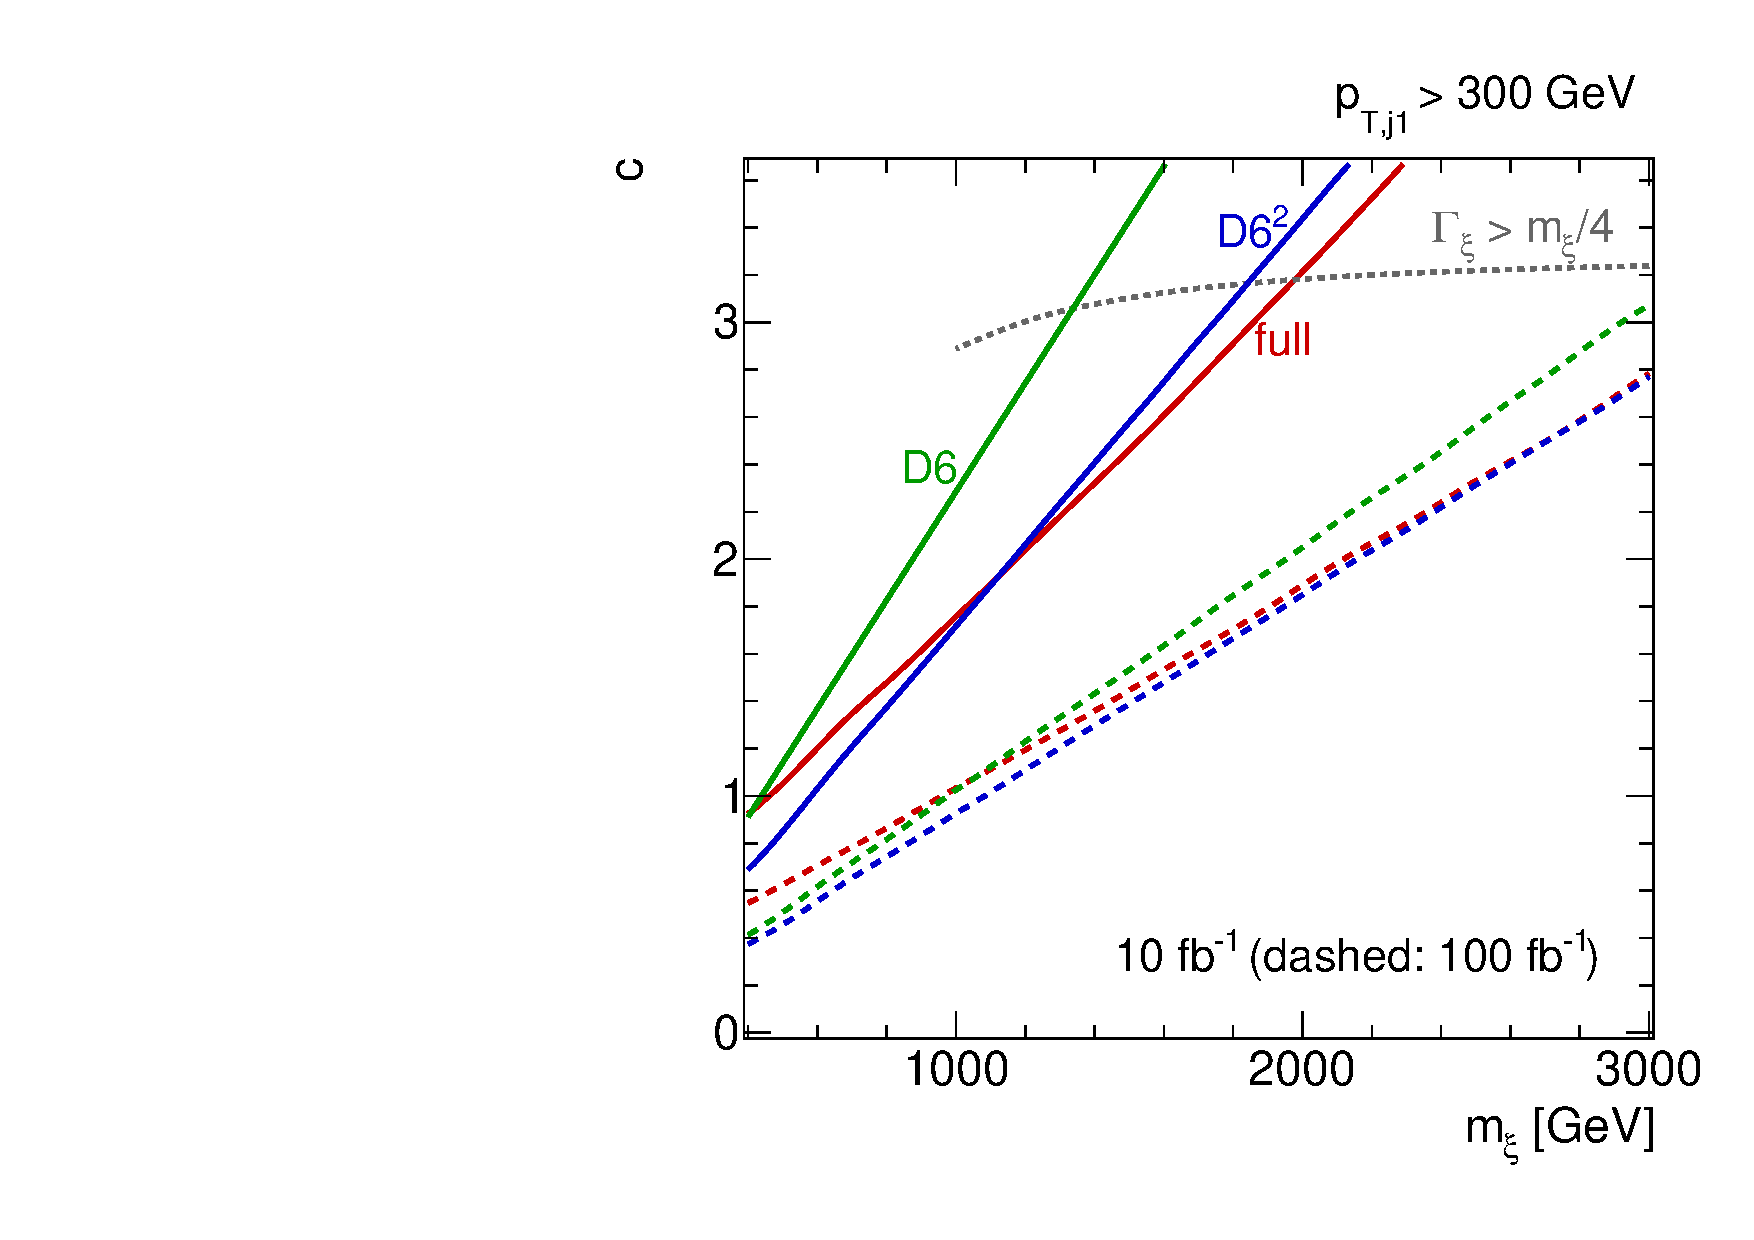
\includegraphics[width=0.43\textwidth]{fig/validity/WBF_limits_300.pdf} 
  \caption{Expected limits on a two-dimensional slice of the vector
    triplet parameter space. We show the analysis based on the event
    numbers in $150~\gev < p_{T,j_1} < 300~\gev$ (left) and based on
    the tail $p_{T,j_1} > 300$~GeV.}
  \label{fig:validity_limits}
\end{figure}
%------------------------------------------------------------


In the middle panels of Fig.~\ref{fig:validity_squared_WBF} we see that indeed
the $p_{T,h}$ distribution looks almost identical to $p_{T,j_1}$. Both
of them can be traced back to the unobservable virtualities of the
weak bosons. Due to the preferred collinear direction of the
quark-vector splittings, the $W$-mediated and $Z$-mediated diagrams
populate very different parton-level phase-space regions, with
basically no interference between them.  We can thus define the
virtuality variable~\cite{gino,polarized_ww}
%
\begin{align}
  q =
  \begin{cases}
    \max\left(   \sqrt{ | (p_{u'} - p_{d})^2 | } \, , \, \sqrt{ | (p_{d'} - p_{u})^2 | }  \right) & \text{for $W$-like phase-space points,} \\
    \max\left(   \sqrt{ | (p_{u'} - p_{u})^2 | } \, , \, \sqrt{ | (p_{d'} - p_{d})^2 | }  \right)  & \text{for $Z$-like phase-space points,}
  \end{cases}
  \label{eq:virt}
\end{align}
%
with the distribution shown in the bottom panels of
Fig.~\ref{fig:validity_squared_WBF}. Comparing it to $p_{T,h}$ and $p_{T,j_1}$ we see
essentially the same behavior.  The strong correlation of $q$ with
the observable transverse momenta of the leading tagging jet and the
Higgs is explicitly shown in Fig.~\ref{fig:validity_virt_corr}.\bigskip

Finally, we compare expected exclusion limits on the vector triplet in
the absence of a signal, based on the full model vs the dimension-6
approach.  For the process shown in Eq.\;\eqref{eq:def_wbf} we
multiply the cross sections with a branching ratio
$\br(h \to 2\ell 2\nu) \approx 0.01$.  We disregard non-Higgs
backgrounds as well as parton-shower or detector effects.  We then
count events in two high-energy bins of the $p_{T,j_1}$ distributions,
defining a parameter point to be excluded if $S/\sqrt{S+B} > 2$.
While this statistical analysis is not designed to be realistic, it
illustrates how the validity of our dimension-6 approach affects
possible limits.  For our limit setting procedure we choose a
two-dimensional plane defined by $m_\xi$ versus a universal coupling
rescaling $c$,
%
\begin{align}
  g_V = 1 \; , \qqquad 
  c_H = c \; , \qqquad 
  c_F = \frac {g_V^2}{2g^2} \, c \; , \qqquad 
  c_{HHVV} = c^2 \; .
\end{align}
%
This reduces the list of generated dimension-6 operators to
%
\begin{align}
  f_{WW} = f_{BW} = \frac {c^2} {2g^2} \qquad \text{and} \qquad  f_W = - \frac {c^2} {g^2} \,,
\end{align}
%
and all dimension-6 deviations scale like $c^2/m_\xi^2$. To avoid
effects from strongly interacting theories we limit our analysis to
$\Gamma_{\xi}/m_{\xi} < 1/4$.

In the left panel of Fig.~\ref{fig:validity_limits} we see that based on event
numbers in the range $150~\text{GeV} < p_{T,j_1} < 300~\text{GeV}$,
the dimension-6 approximation with the squared terms gives the
same limits as the full model, as long as we ensure that the new
resonance remains narrow.  In the high-energy tail
$p_{T,j_1} > 300$~GeV including the squared terms also improves the validity of
the dimension-6 approach, but it only leads to identical limits for
large $m_\xi$, combined with strong couplings. Indeed, limiting the
momentum transfer of events for example through an upper limit on
$p_{T,j}$ is well known to reduce the dependence on model
assumptions~\cite{spins1,spins2}.

Just as for the $Vh$ production process, at least as long as the event
numbers remain small the square of the dimension-6 operators always
improves the agreement with the full theory in weak boson fusion. With
improved statistics the differences become smaller and ultimately
negligible, and the question of whether the squared dimension-6
amplitudes should be taken into account is rendered irrelevant.





%%%%%%%%%%%%%%%%%%%%%%%%%%%%%%%%%%%%%%%%%%%%%%%%%%%%%%%%%%%%
\subsection{Realistic tagging jets}
%%%%%%%%%%%%%%%%%%%%%%%%%%%%%%%%%%%%%%%%%%%%%%%%%%%%%%%%%%%%

%------------------------------------------------------------
\begin{figure}[t]
  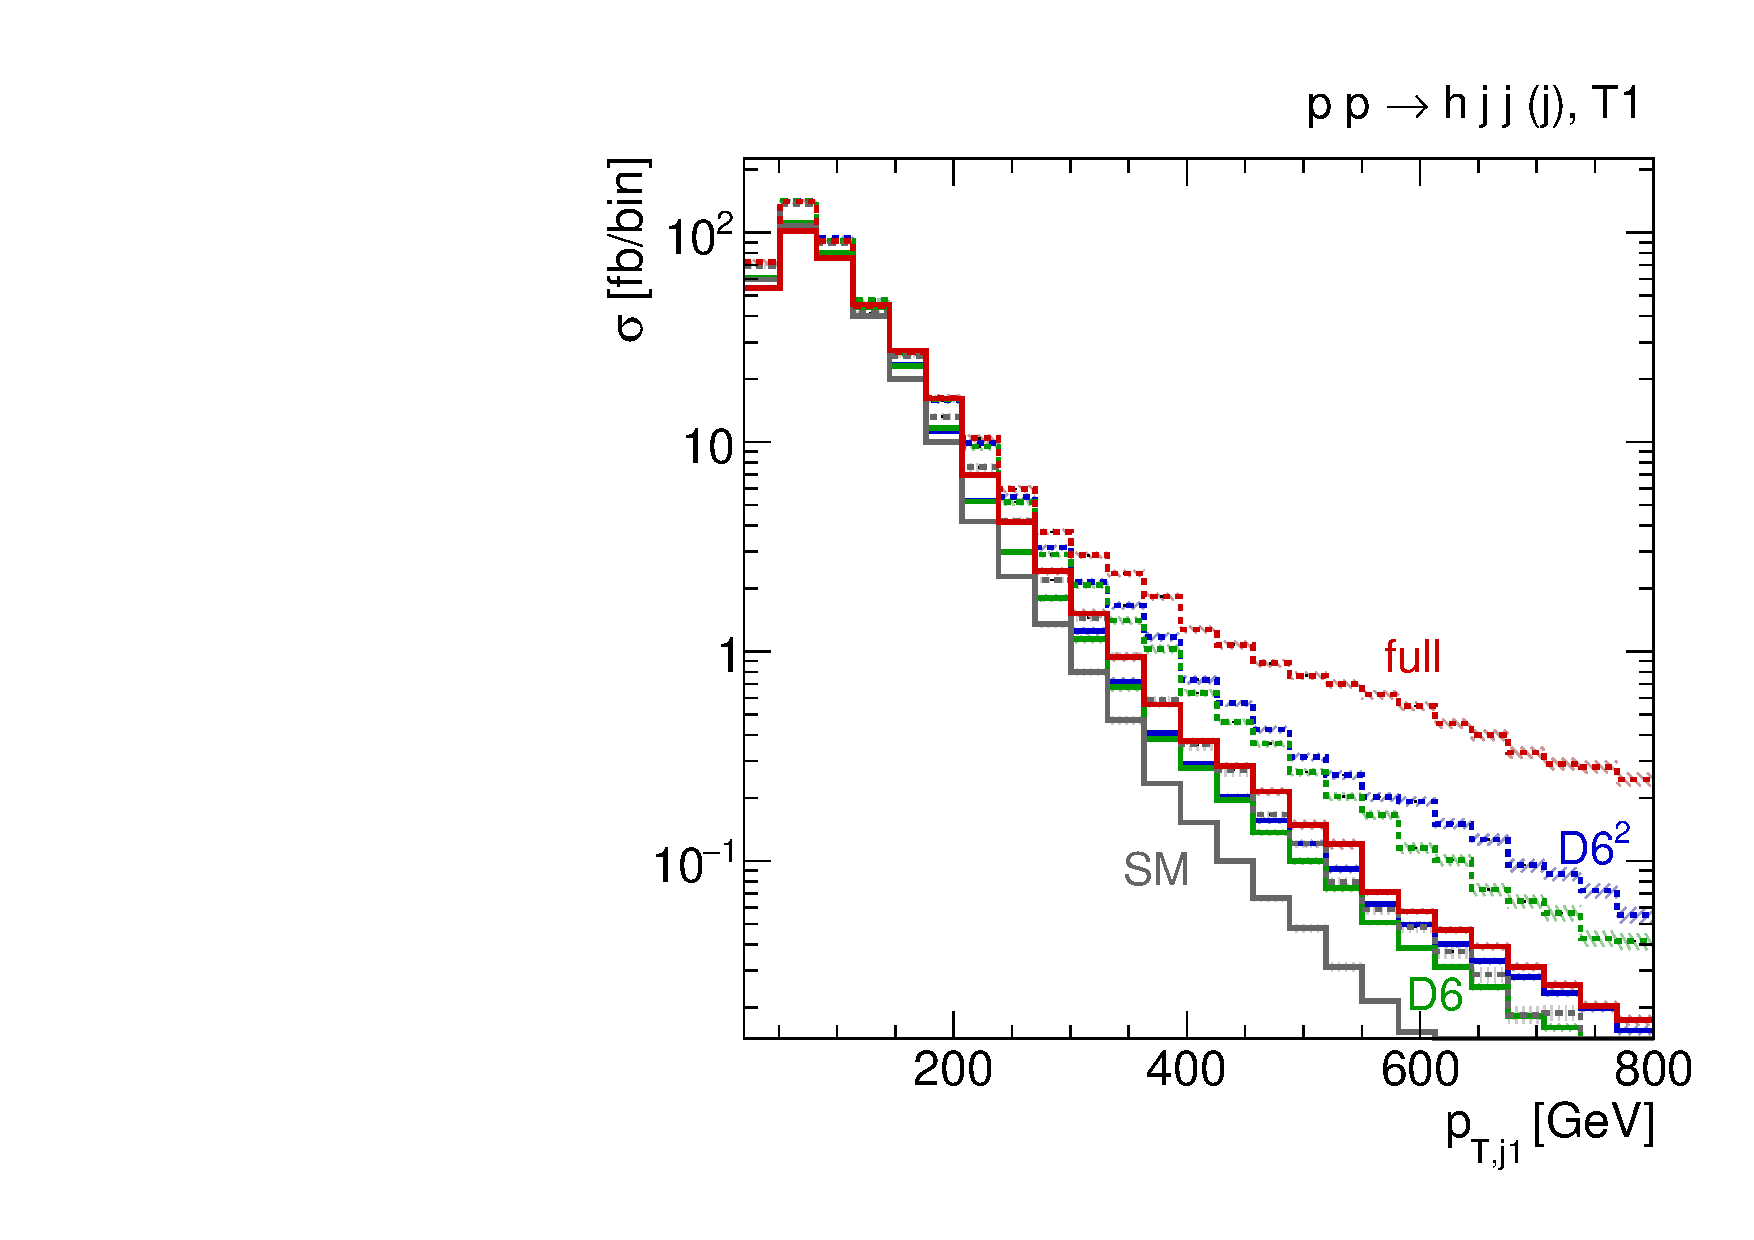
\includegraphics[width=0.43\textwidth]{fig/validity/WBF_realistic_T1_j1pt.pdf}
  \hspace*{0.05\textwidth}
  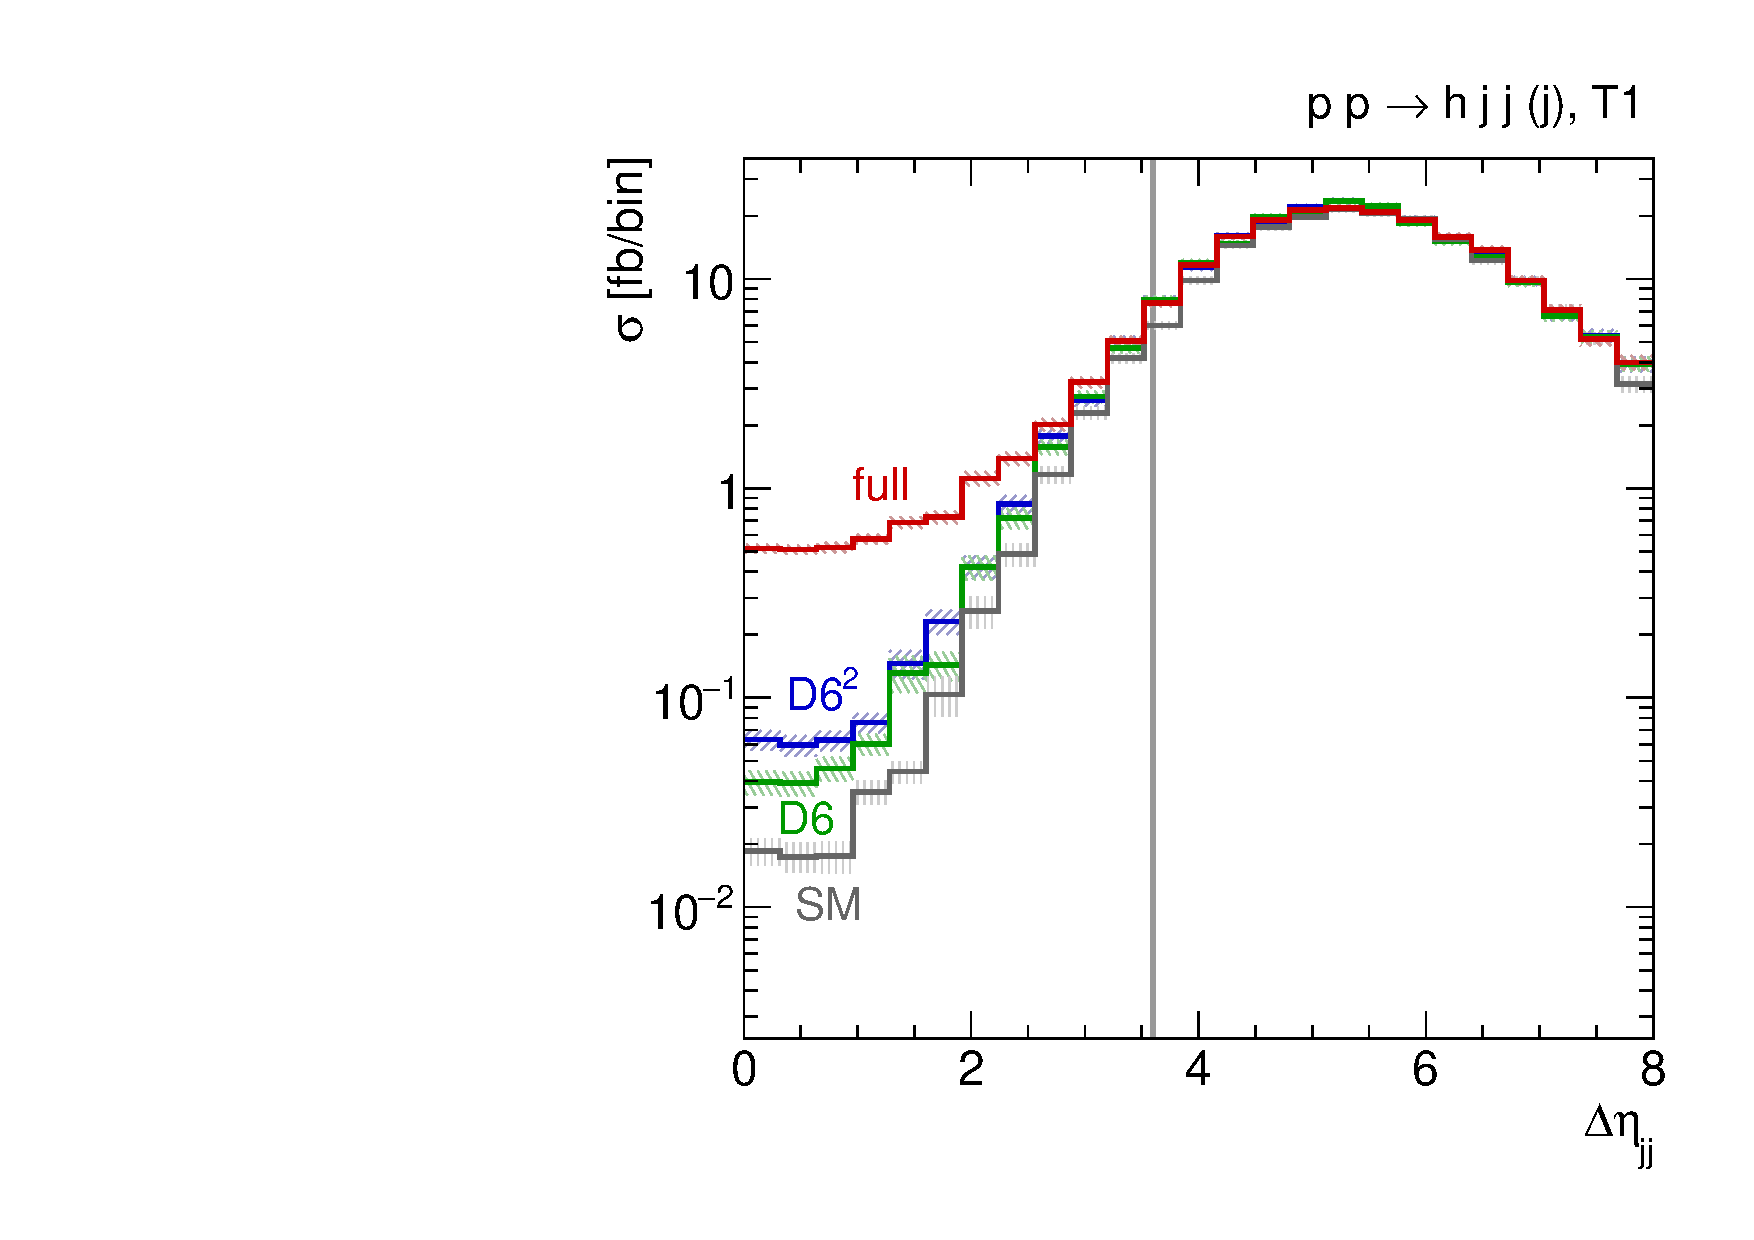
\includegraphics[width=0.43\textwidth]{fig/validity/WBF_realistic_T1_deltaEtaJJ.pdf}
  \caption{WBF distribution at hadron level. Left: $p_{T,j_1}$
    distribution based on the full process, the dashed lines show the
    distributions based on WBF diagrams only and without a
    $\Delta \eta_{jj}$ cut. Right: $\Delta \eta_{jj}$ based on WBF
    diagrams only, the vertical line marks the standard WBF cut
    following Eq.\;\eqref{eq:wbf_cuts}.}
  \label{fig:validity_realistic_jets}
\end{figure}
%------------------------------------------------------------

Before we attempt to further improve the description of the full vector
triplet model for example in the benchmark point T1, we briefly test
if the parton-level effects described above survive a realistic environment.
We add a parton shower and jet reconstruction now for the full
process
%
\begin{align}
  p p \to h \; j j \, (+j) \; ,
\end{align}
%
simulated in \toolfont{MadGraph}~\cite{madgraph}.  Parton showering is
performed by \toolfont{PYTHIA6}~\cite{pythia} using the $k_T$-jet MLM
matching scheme~\cite{mlm} with a minimum $k_T$ jet measure between
partons of \toolfont{xqcut}=20~GeV. \toolfont{Fastjet}~\cite{fastjet}
is used to construct jets based on the $k_T$ algorithm with $R = 0.4$. We do not
include a Higgs decay because we are only interested in
production-side kinematics.  The standard WBF cuts then are
%
\begin{align}
  p_{T,j} > 20~\gev \,, \qqquad 
  m_{jj} > 500~\gev \,, \qqquad 
  \Delta \eta_{jj}~>~3.6
\label{eq:wbf_cuts}
\end{align}
%
on the two hardest jets. We veto additional jets with
$p_{T,j} > 20$~GeV between these two tagging jets.  To analyze the
effects of the $\Delta \eta_{jj}$ cut~\cite{spins2}, we generate
additional samples explicitly excluding Higgs-strahlung diagrams, in
spite of the fact that it might break gauge invariance.

In Fig.~\ref{fig:validity_realistic_jets} we show that the distributions are
generally robust under parton shower and jet reconstruction, but two
complications arise.  First, on-shell $\xi$ production contributes to
this process and is not entirely removed by the WBF cuts in
Eq.\;\eqref{eq:wbf_cuts}, leading to visible differences between the
full and effective model already at low momenta. Such a resonance peak
would be easy to identify experimentally and does not present a major
problem for the dimension-6 approximation.

Second, the tension between the full model and the dimension-6
approximation at large momenta now remains below $10~\%$.  This means
that the $\Delta \eta_{jj}$ cut not only removes large contributions
from Higgs-strahlung--like diagrams, it also gets rid of phase-space
regions where the full model and the dimension-6 description differ
the most.  At the same time, the $\Delta \eta_{jj}$ removes some of
its well-known discrimination power for new physics effects versus the
Standard Model~\cite{spins2}.




%%%%%%%%%%%%%%%%%%%%%%%%%%%%%%%%%%%%%%%%%%%%%%%%%%%%%%%%%%%%
\subsection{Towards a simplified model}
\label{sec:validity_simplified}
%%%%%%%%%%%%%%%%%%%%%%%%%%%%%%%%%%%%%%%%%%%%%%%%%%%%%%%%%%%%

%------------------------------------------------------------
\begin{figure}[t]
  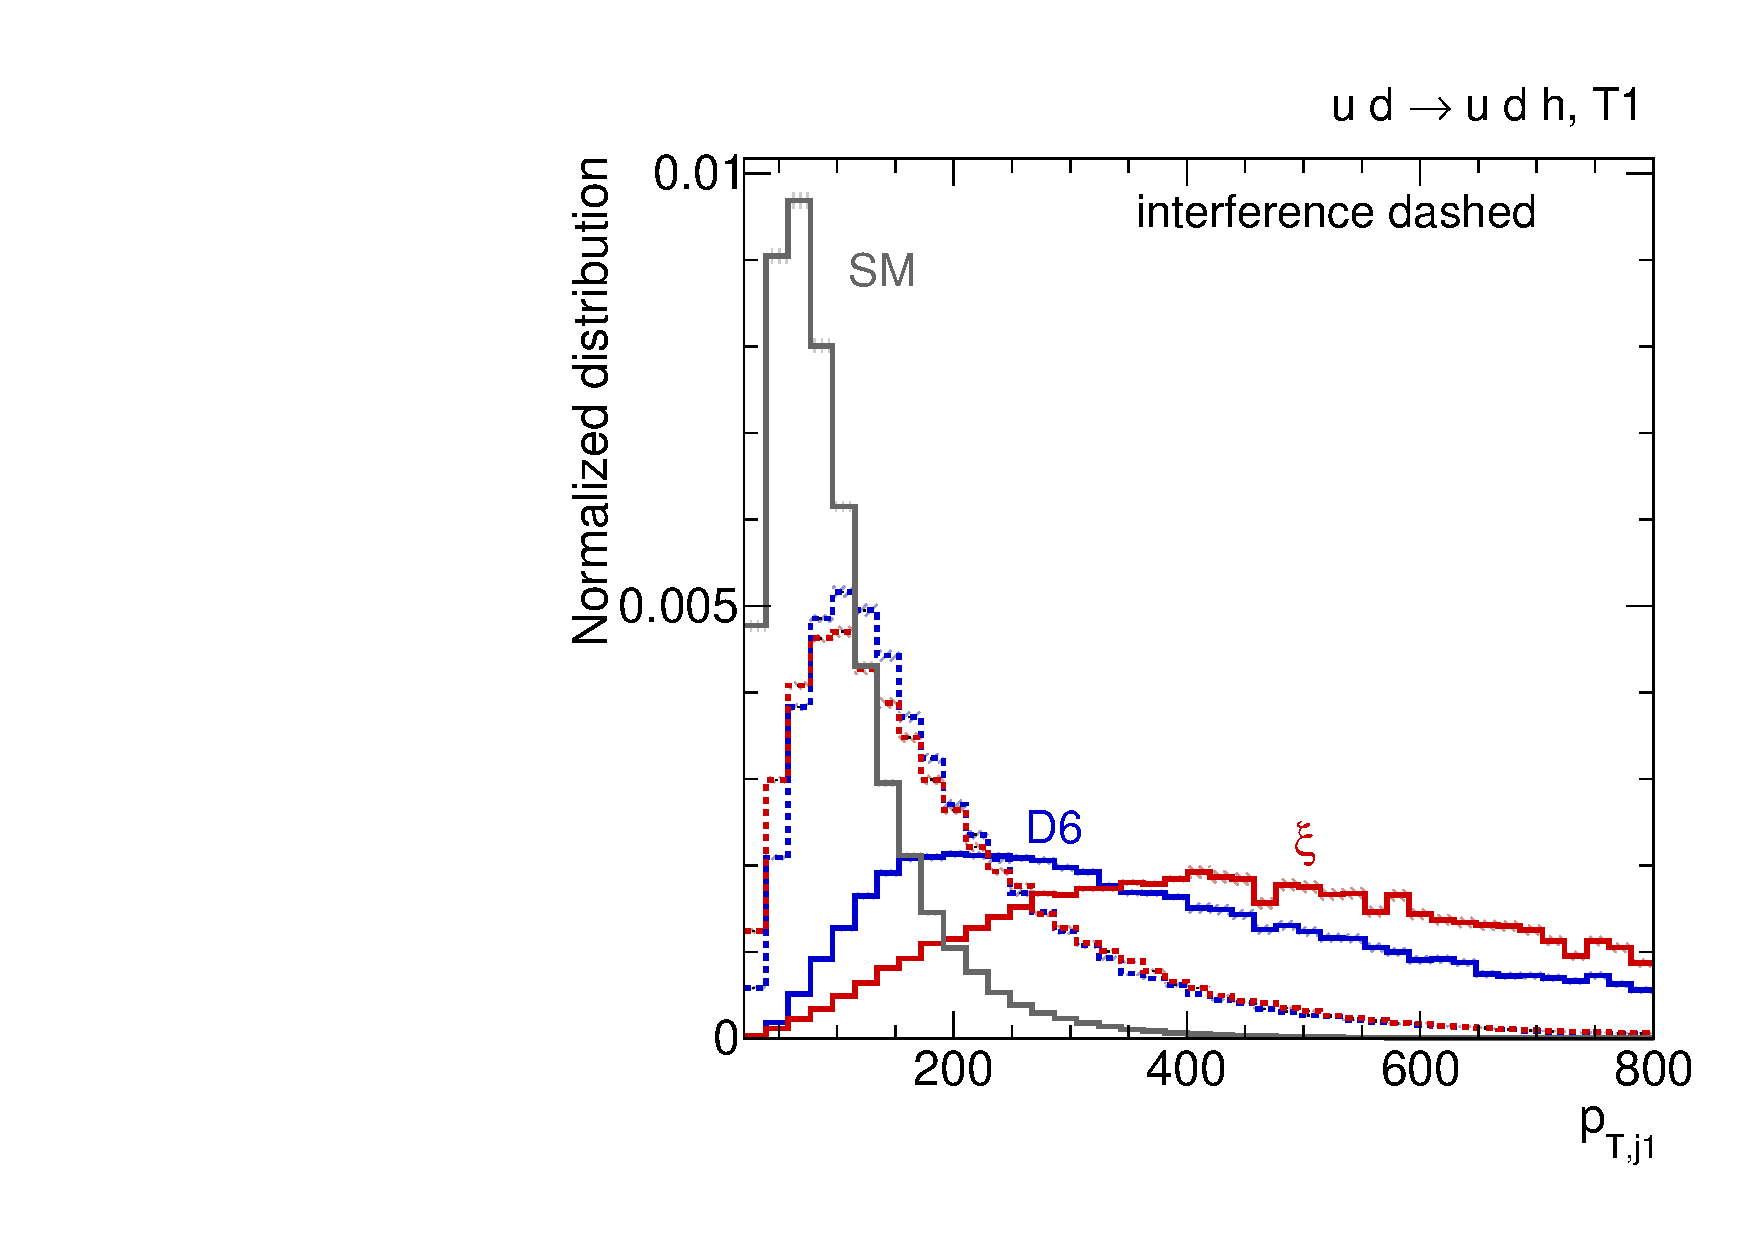
\includegraphics[width=0.43\textwidth]{fig/validity/WBF_separate_T1_j1pt.pdf} 
  \hspace*{0.05\textwidth}
  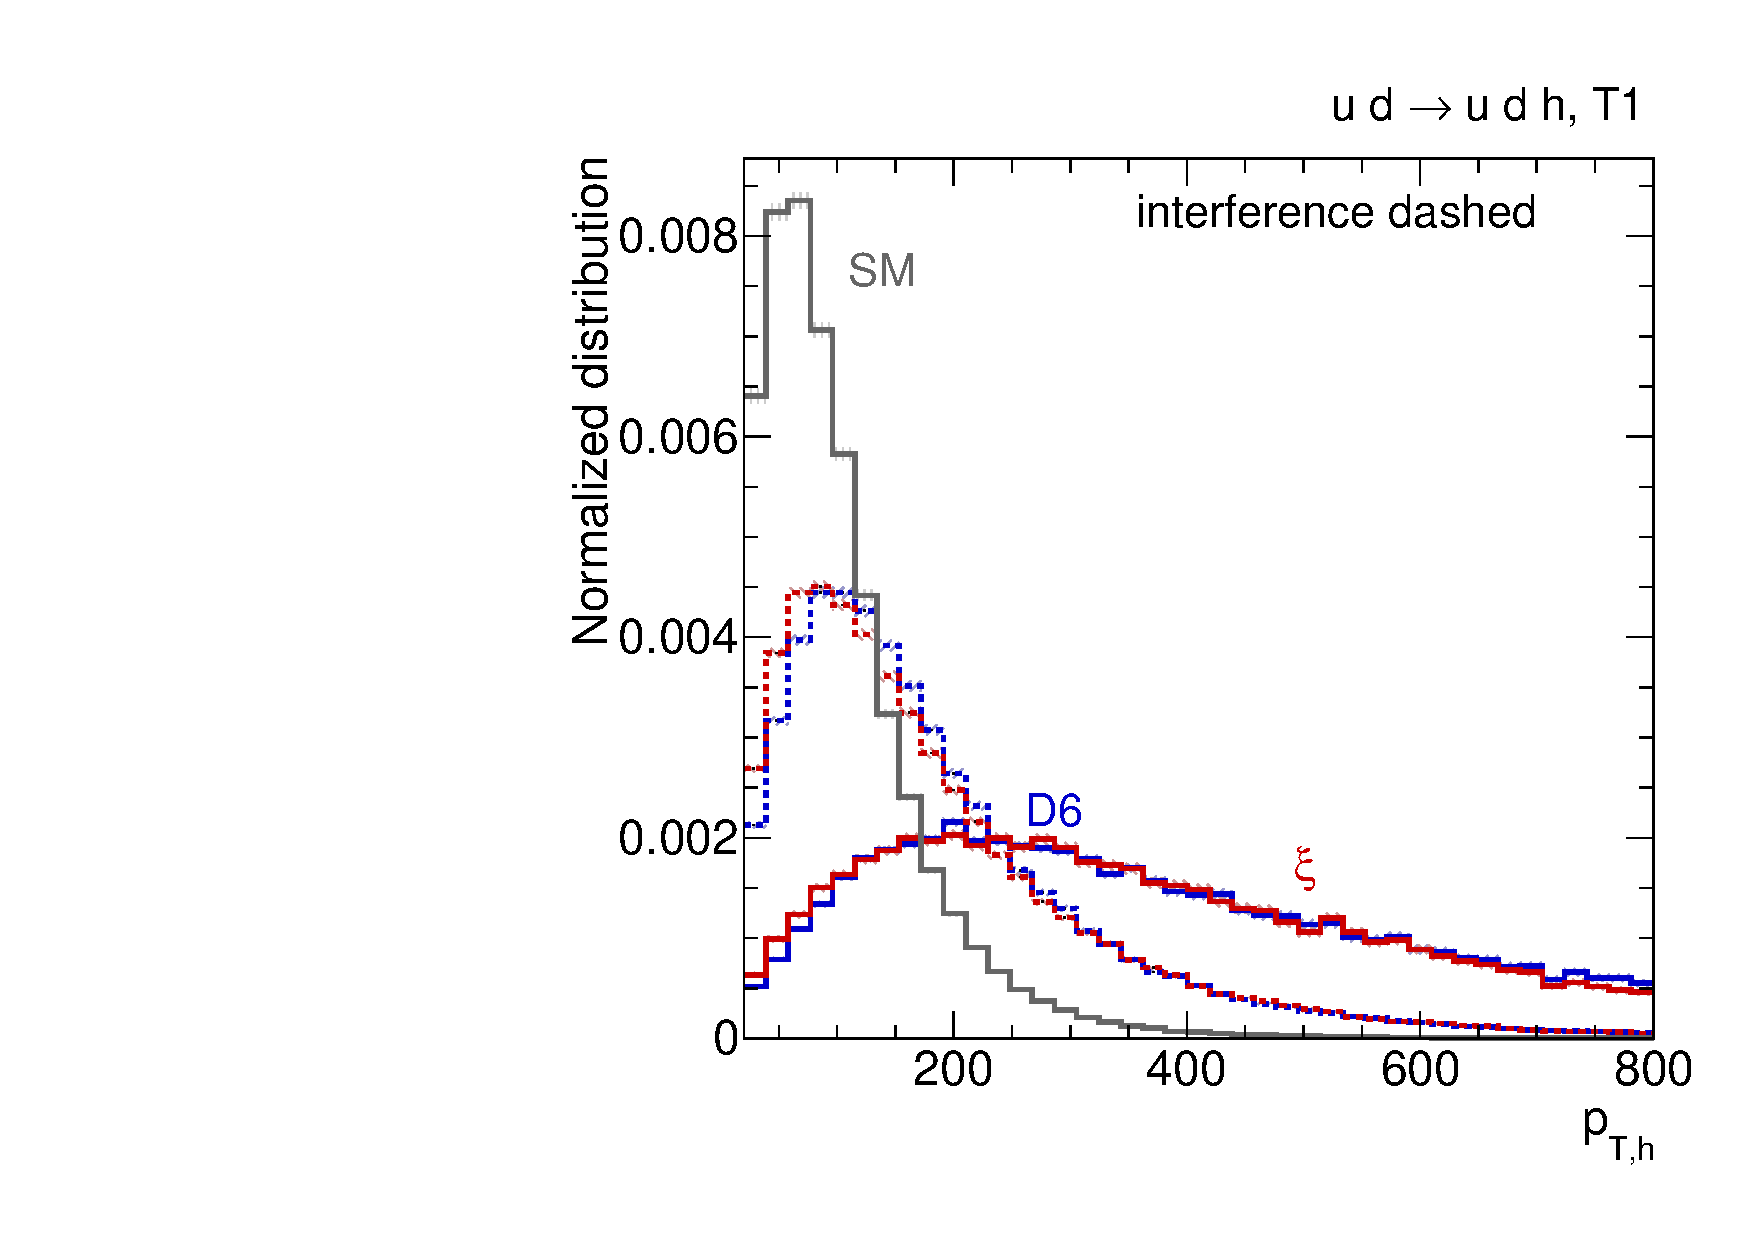
\includegraphics[width=0.43\textwidth]{fig/validity/WBF_separate_T1_Hpt.pdf}\\
  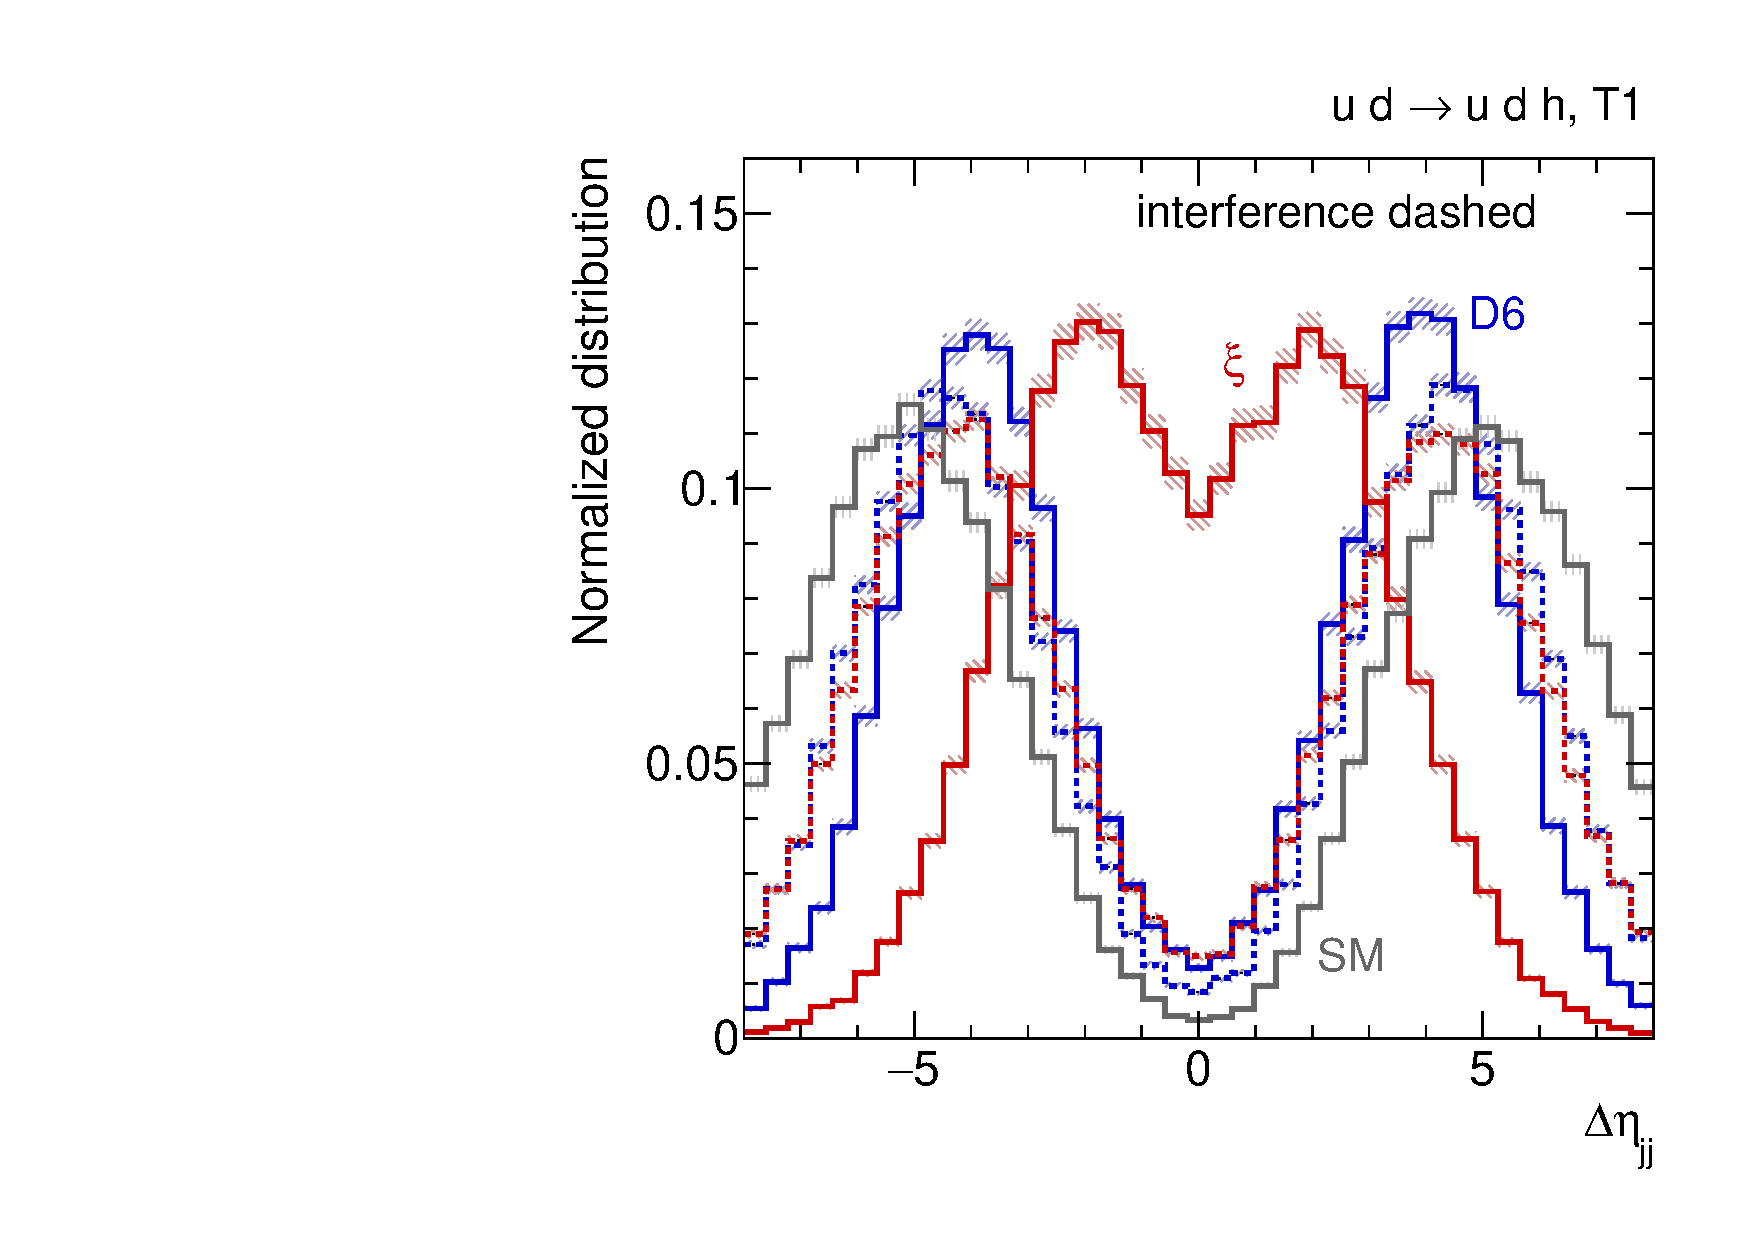
\includegraphics[width=0.43\textwidth]{fig/validity/WBF_separate_T1_deltaEtaJJ.pdf} 
  \hspace*{0.05\textwidth}
  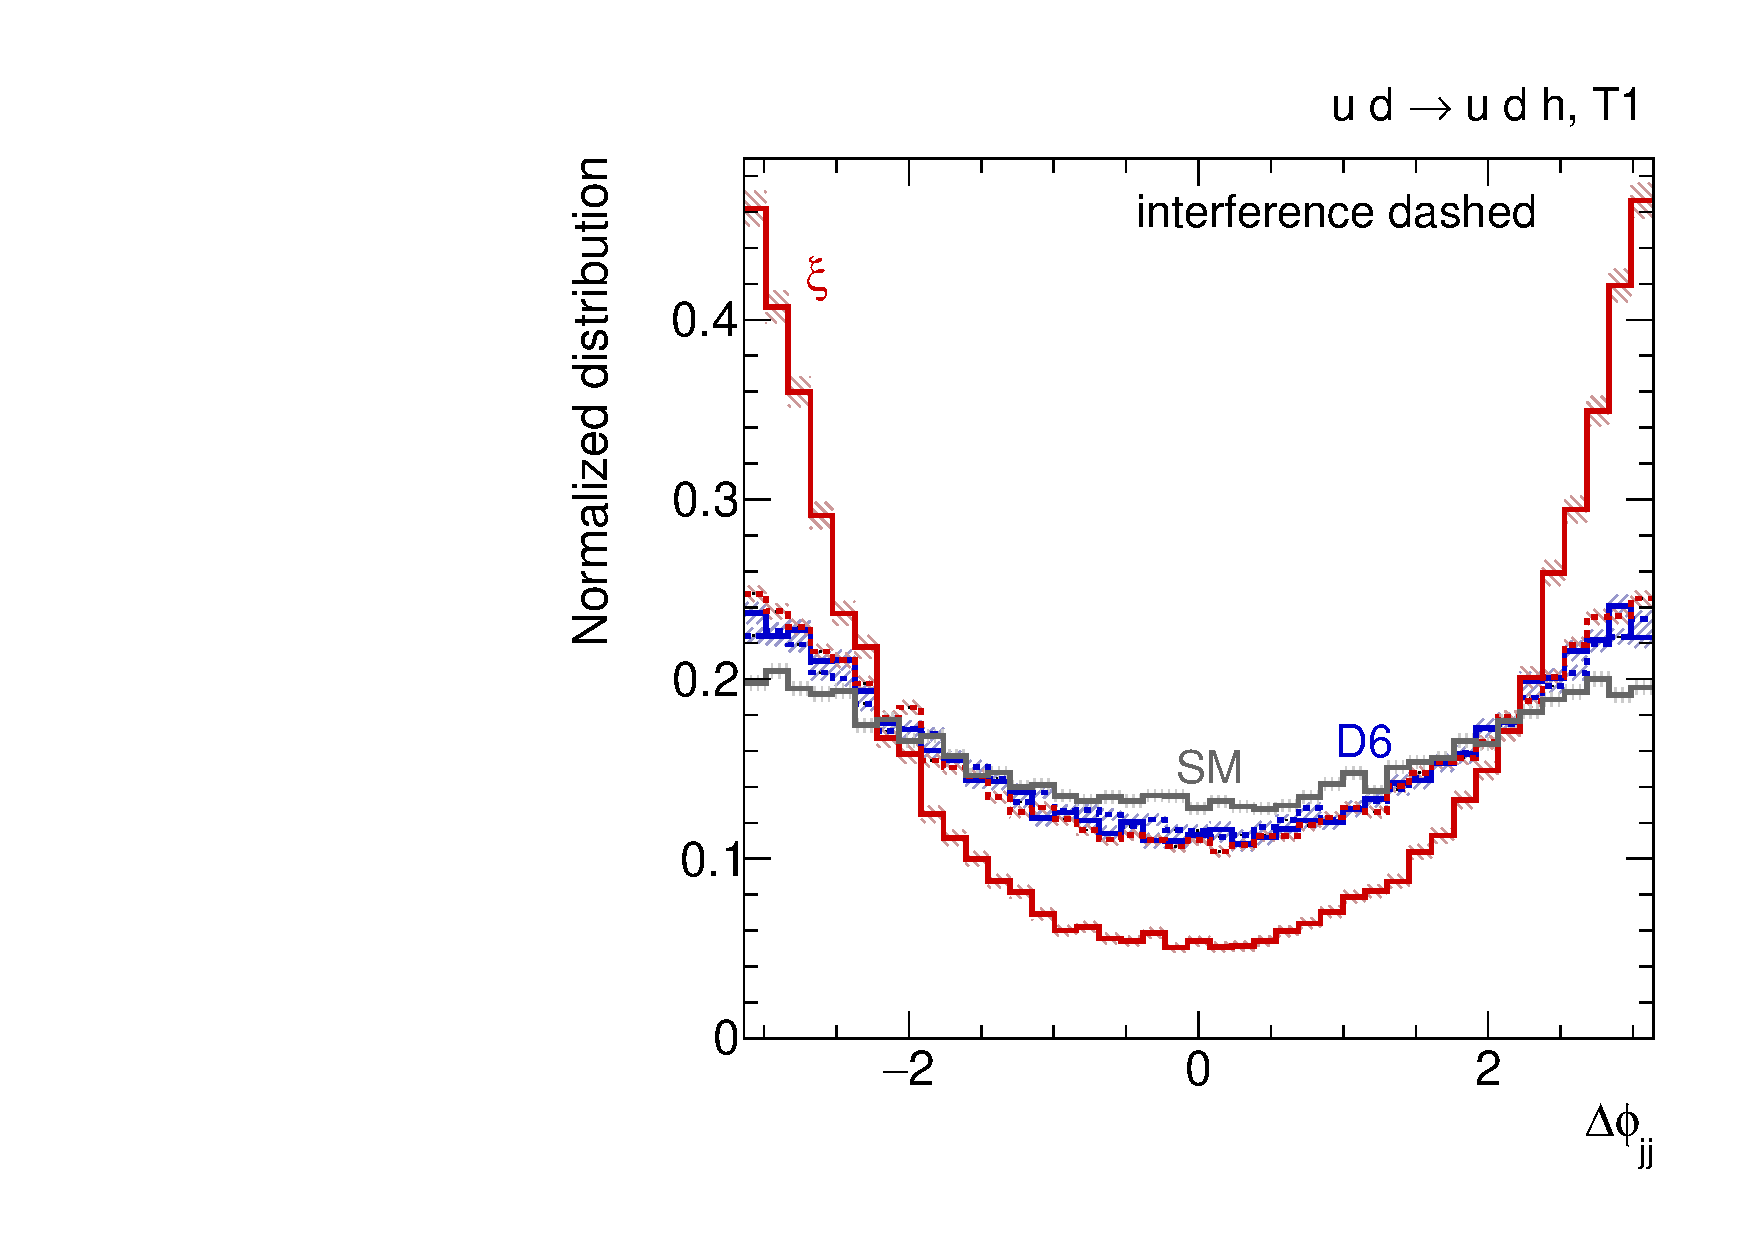
\includegraphics[width=0.43\textwidth]{fig/validity/WBF_separate_T1_deltaPhiJJ.pdf}
  \caption{Normalized WBF distributions of the tagging jets. We separate
    the squared new-physics amplitudes, shown as solid lines, from the
    interference with the SM-like diagrams (dashed).}
  \label{fig:validity_squared_separate}
\end{figure}
%------------------------------------------------------------

In the first part of the paper we have shown where in phase space a
dimension-6 description of LHC observables breaks down, both for $Vh$
production and for weak boson fusion. For $Vh$ production with its
simple $2 \to 2$ kinematics problems are clearly linked to a possible
$s$-channel resonance, as seen in Eq.\;\eqref{eq:breakdown_vh}.  For
weak boson fusion there appears no resonance, but the result of
Eq.\;\eqref{eq:breakdown_wbf} suggests that the new states in the
$t$-channel have a similar effect.  In Fig.~\ref{fig:validity_squared_separate}
we show different tagging jet distributions, separating the Feynman
diagrams including the heavy $\xi$ states. In particular for the
critical $p_{T,j_1}$ distribution, the $\Delta \eta_{jj}$
distribution, and the $\Delta \phi_{jj}$ distribution these diagrams
are only very poorly described by the dimension-6 approach. In
practice this is not a problem because these contributions are
strongly suppressed by the heavy mass $m_\xi$, but it poses the
question how we can improve the agreement. The obvious solution to
these problems in the $s$-channel of $Vh$ production and in the
$t$-channel of weak boson fusion is a simplified
model~\cite{simp,simp_higgs}. A new vector field mixing with the weak
bosons as described by the Lagrangian shown in
Eq.\;\eqref{eq:lag-vectortriplet} is such a simplified model, but its
structure is still relatively complex. Obviously, an additional heavy
scalar with mass around $m_\xi$ and the appropriate couplings will
improve the $2 \to 2$ kinematics for $Vh$ production. The question we
want to study in this section is if such a scalar can also improve the
weak boson fusion kinematics.



%%%%%%%%%%%%%%%%%%%%%%%%%%%%%%%%%%%%%%%%%%%%%%%%%%%%%%%%%%%%
\subsubsection*{A pseudo-scalar as a simplified vector}
%%%%%%%%%%%%%%%%%%%%%%%%%%%%%%%%%%%%%%%%%%%%%%%%%%%%%%%%%%%%

The simplest simplified model we can write down includes one new
massive scalar $S$ with a Higgs portal and a Yukawa coupling. 
However, a scalar state will not interfere with the Standard Model
diagrams. In analogy to the CP properties of the Goldstone mode
contributing to the massive $Z$ boson we define our simplified model
with a pseudo-scalar state as
%
\begin{align}
\mathcal{L} \supset 
  \frac{1}{2} (\partial_\mu S)^2 
- \frac{m_S}{2} S^2 
+ \sum_\text{fermions} g_F \; S \overline{F} \gamma_5 F 
+ g_S \; S^2 \phi^\dagger \phi \,.
  \label{eq:simplified_model}
\end{align}

%------------------------------------------------------------
\begin{figure}[t]
  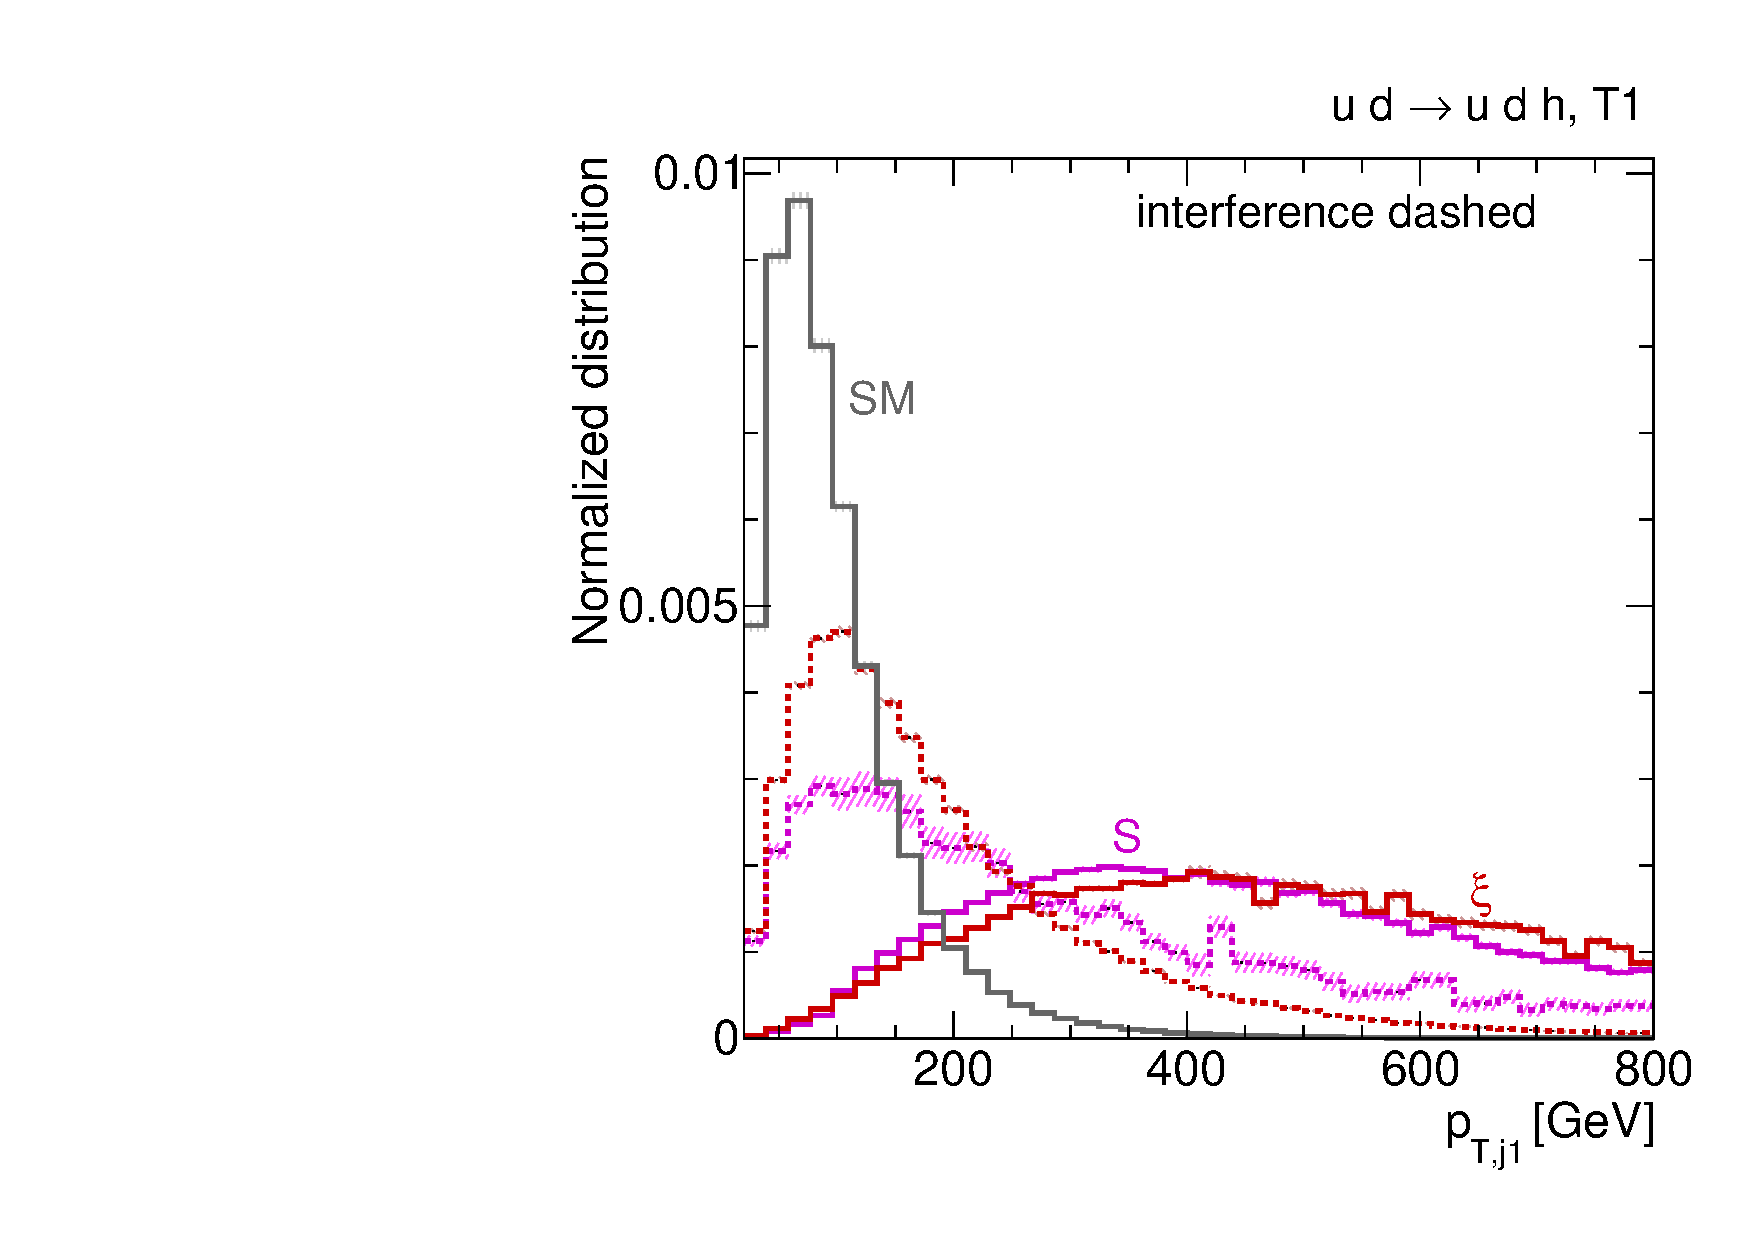
\includegraphics[width=0.43\textwidth]{fig/validity/WBF_simplified_j1pt.pdf}
  \hspace*{0.05\textwidth}
  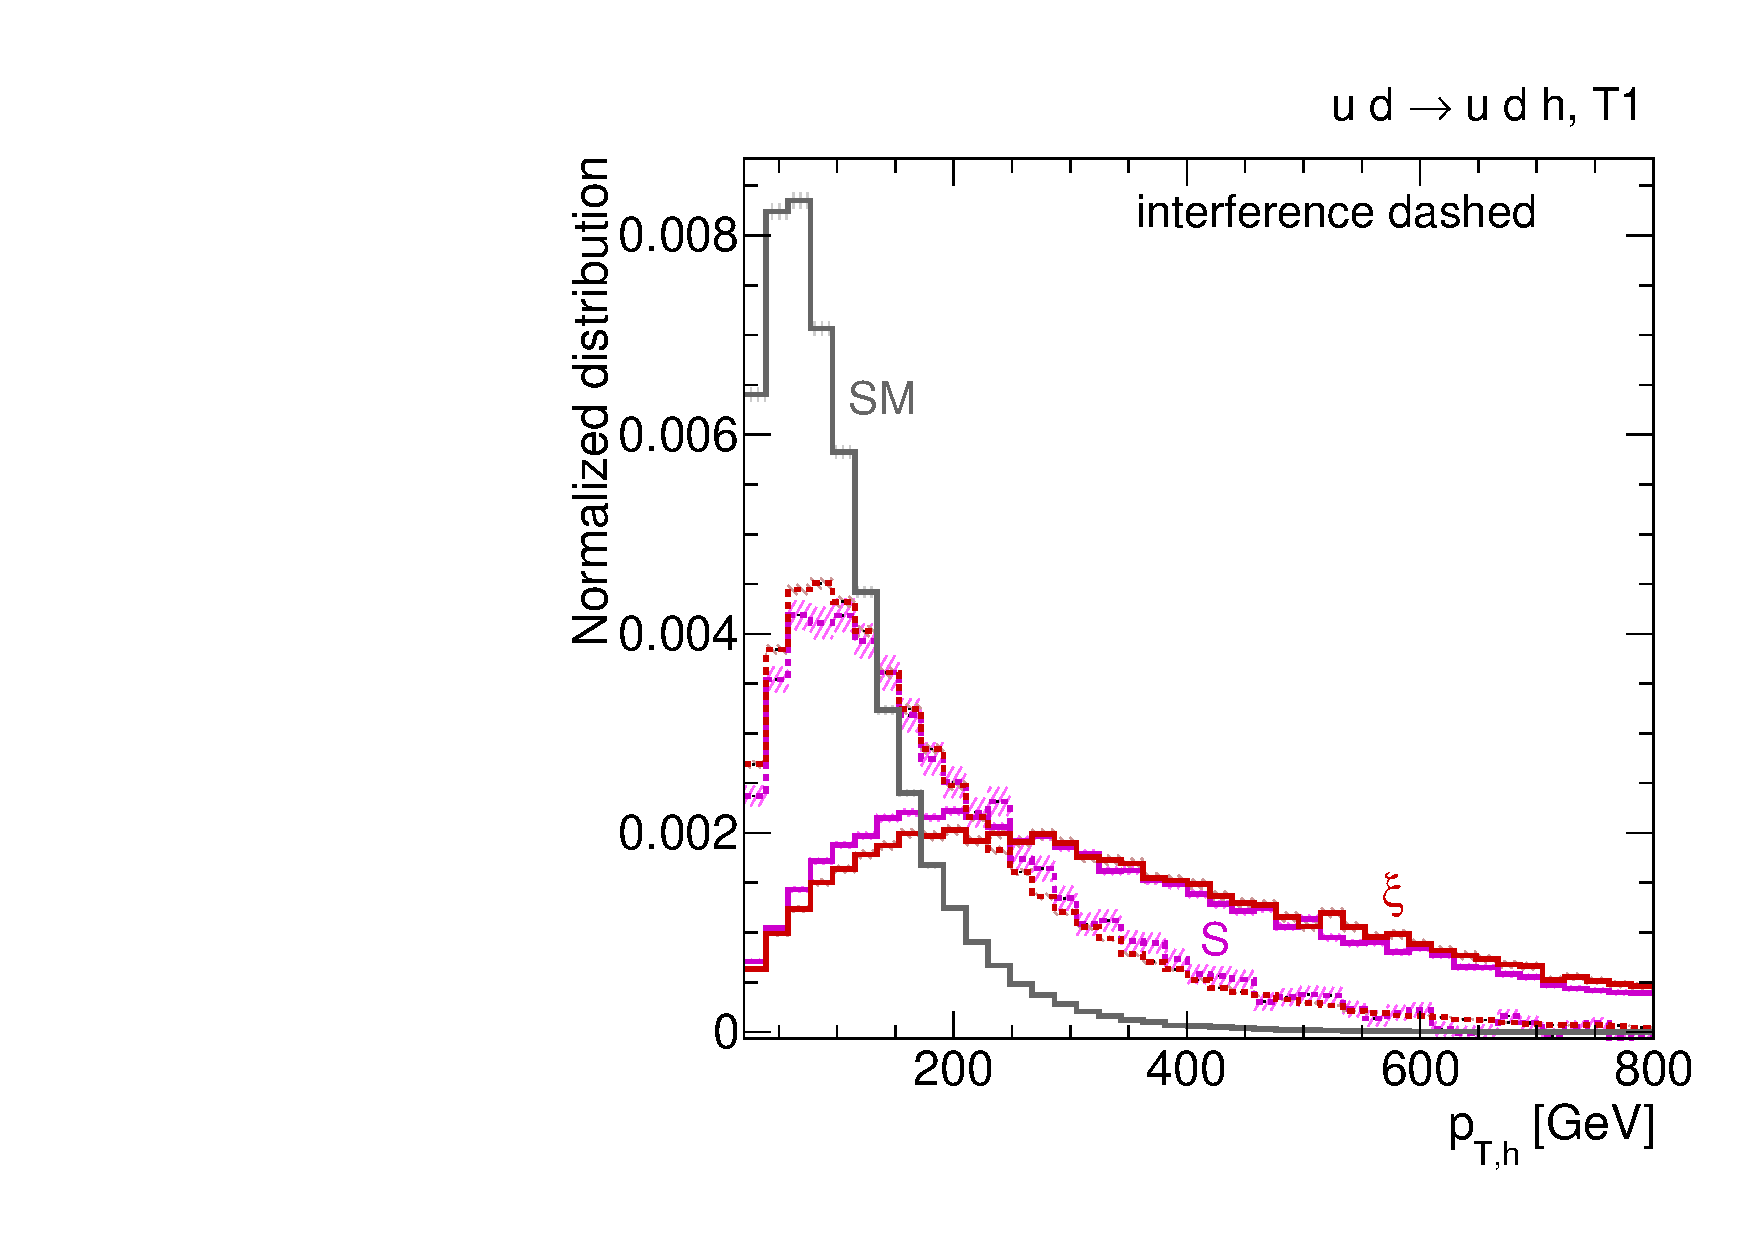
\includegraphics[width=0.43\textwidth]{fig/validity/WBF_simplified_Hpt.pdf} \\
  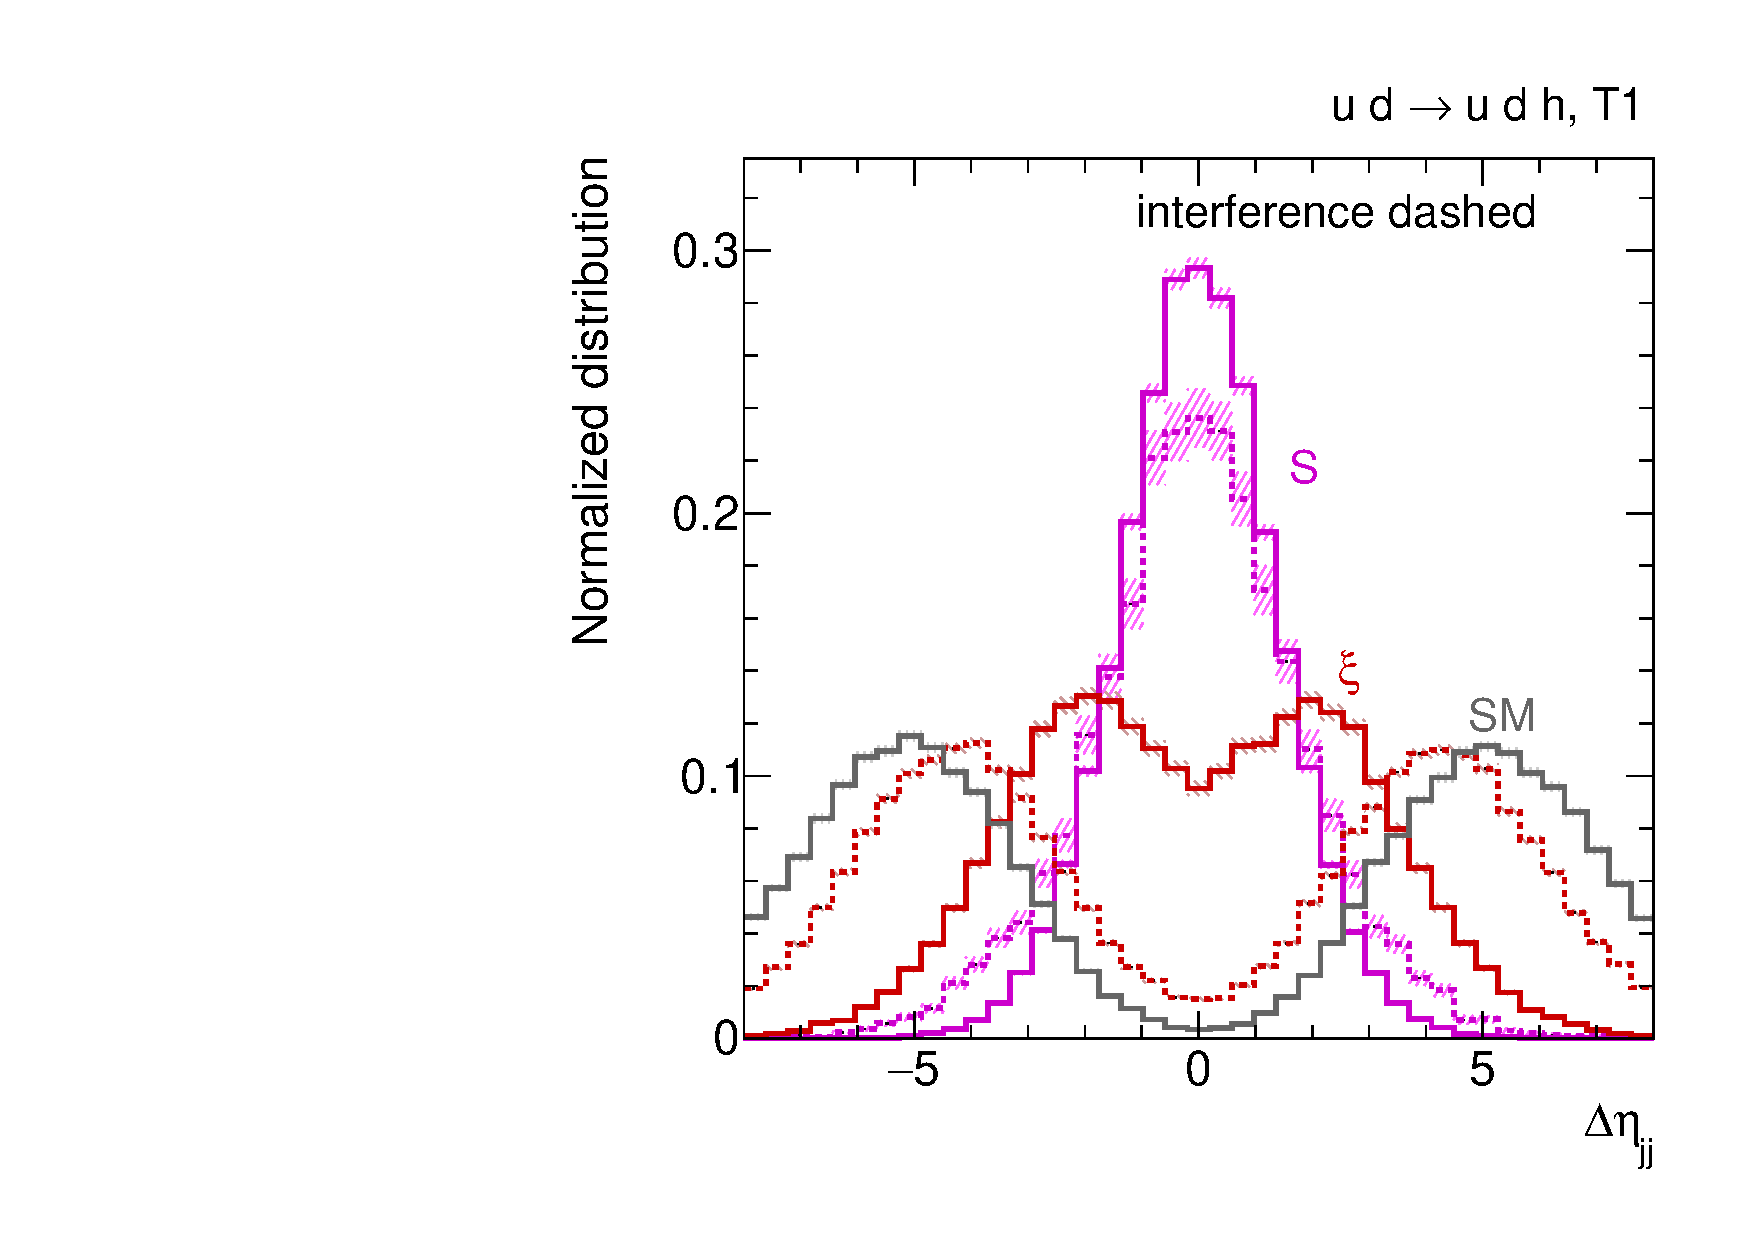
\includegraphics[width=0.43\textwidth]{fig/validity/WBF_simplified_deltaEtaJJ.pdf}
  \hspace*{0.05\textwidth}
  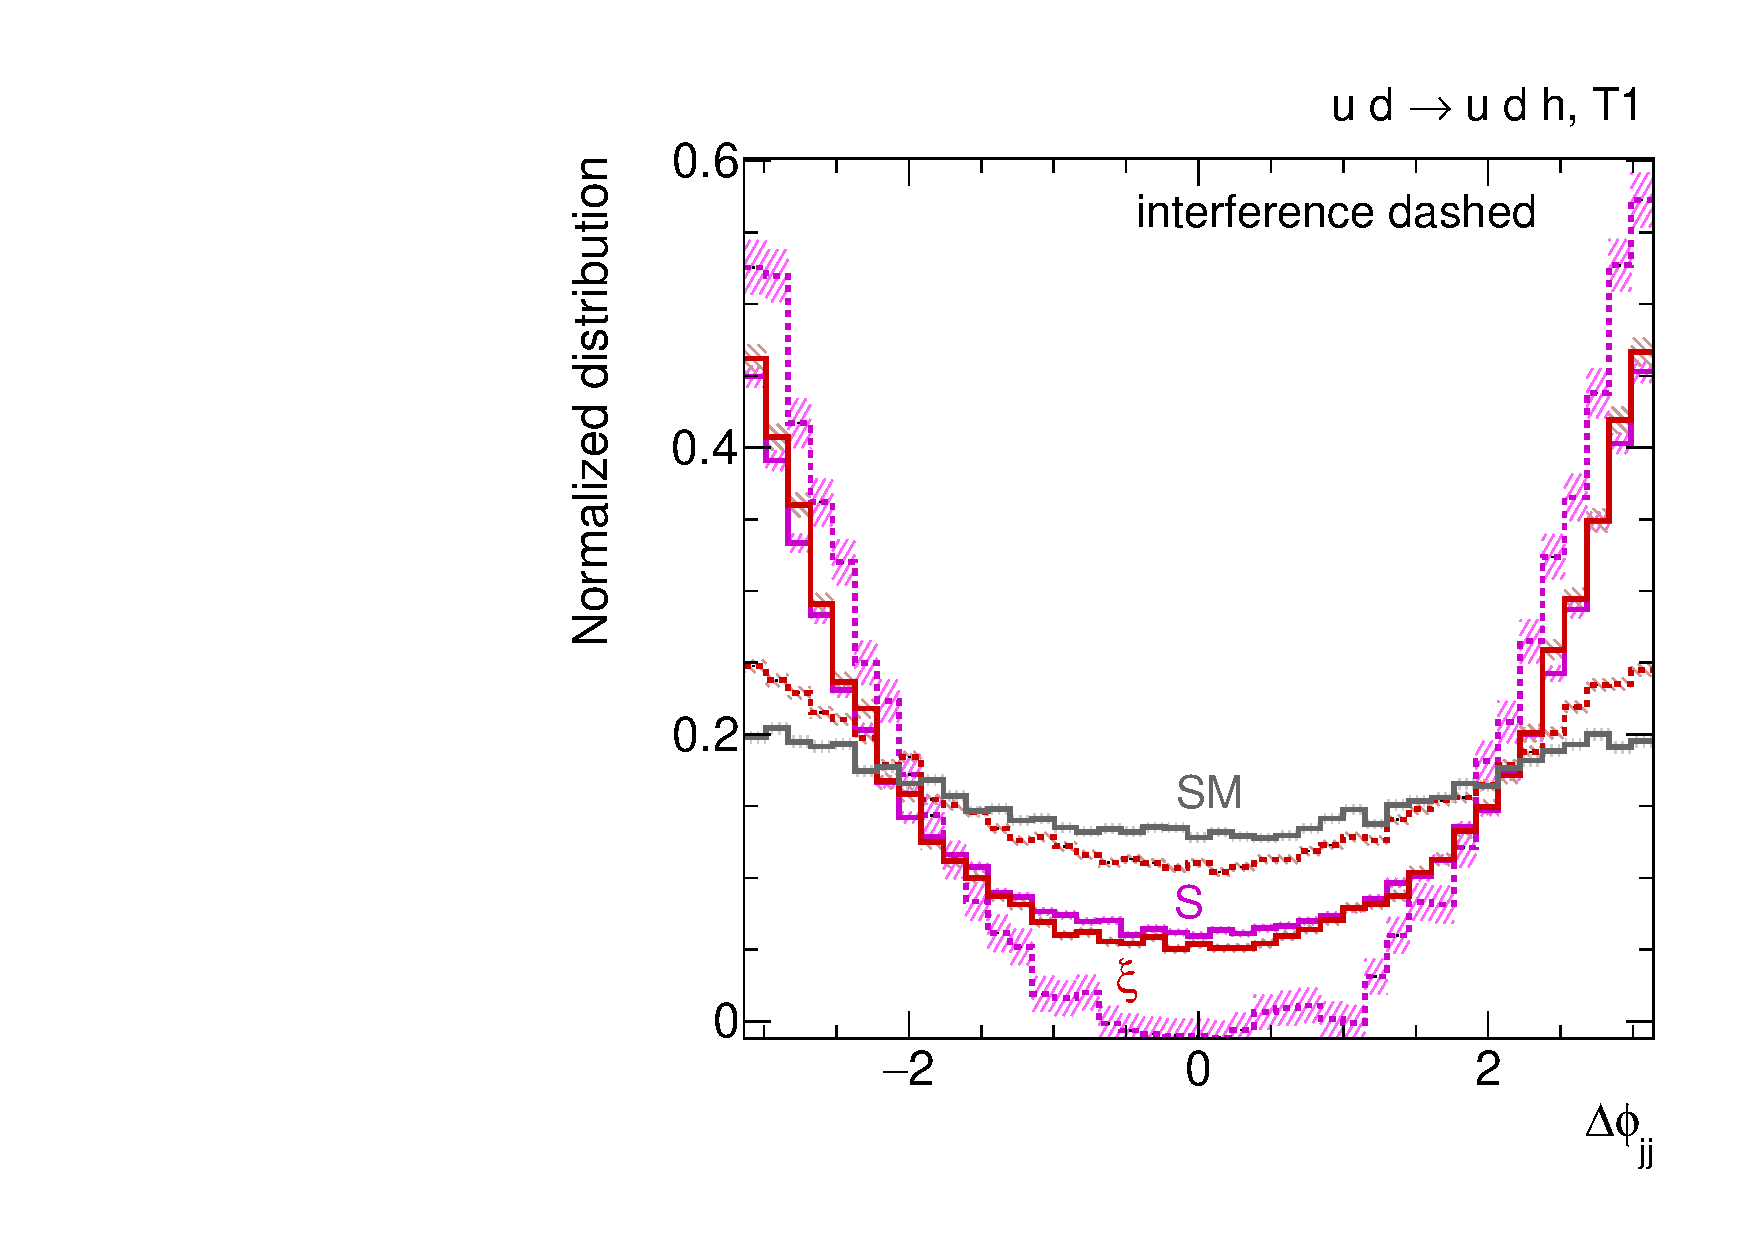
\includegraphics[width=0.43\textwidth]{fig/validity/WBF_simplified_deltaPhiJJ.pdf}
  \caption{Normalized WBF distributions for a scalar simplified model
    defined in Eq.\;\eqref{eq:simplified_model} vs the vector triplet
    benchmark.}
  \label{fig:validity_simplified}
\end{figure}
%------------------------------------------------------------

In Fig.~\ref{fig:validity_simplified} we show the same WBF distributions as in
Fig.~\ref{fig:validity_squared_separate}, but including the simplified scalar
model. For the $p_{T,j}$ distribution the squared new-physics
amplitudes in the full vector model and the simplified scalar model
indeed agree well, improving upon the dimension-6 description which
breaks down in this distribution.  However, the interference term with
the Standard Model, which is numerically dominant for most of the
distribution and well described in the dimension-6 model, poses a
problem.  The $\Delta \eta_{jj}$ distributions show even poorer
agreement: the spin-1 amplitudes of the Standard Model and the vector
triplet have similar phase-space distributions and give two forward
tagging jets, while the scalar mediator favors central
jets~\cite{spins2}.  The $\Delta \phi_{jj}$ distribution, known to be
sensitive to the tensor structure of the hard $VVh$
interaction~\cite{delta_phi}, exposes similar differences between the
full and simplified model.  Altogether, our simplified scalar model
with its very different $VVh$ interaction structure does improve the
description in the region where the dimension-6 approach breaks down,
but it fails to describe interference patterns and angular
correlations of the tagging jets.



%%%%%%%%%%%%%%%%%%%%%%%%%%%%%%%%%%%%%%%%%%%%%%%%%%%%%%%%%%%%
\subsubsection*{Splitting functions and equivalence theorem}
%%%%%%%%%%%%%%%%%%%%%%%%%%%%%%%%%%%%%%%%%%%%%%%%%%%%%%%%%%%%

We can understand this very different behavior of the scalar
$t$-channel mediator as compared to the vector from the splitting
kernels in the collinear limit.  The matrix element squared for the
weak boson fusion process mediated by pseudo-scalars $S$ has the form
%
\begin{align}
 | \mathcal{M}(qq \to q'q'h) |^2 \propto 
  \frac{g_F^4 \;  t_1 t_2}{(t_1 - m_S^2)^2 \; (t_2 - m_S^2)^2} 
\stackrel{m_S \to 0}{\longrightarrow} \frac{\text{const}}{t_1 t_2} \; ,
\end{align}
%
where $t_1$ and $t_2$ denote the respective momentum flow through each
scalar propagator. For $m_S \to 0$ the Jacobians from the phase-space
integration cancel a possible collinear divergence, while for a light
vector boson a soft and a collinear divergence remains. Unlike in the
usual WBF process, the tagging jets in our simplified scalar model
will not be forward.  The reason for this difference in the
infrared is the (pseudo-)scalar coupling to quarks: since the scalar
carries no Lorentz index, a $q \to q S$ splitting will be expressed in
terms of the momentum combinations $(p_q p_q')$, $p_q^2 = m_q^2$, and
$p_q'^2 = m_q^2$. In the limit of massless quarks only the first term
remains as $t = 2 (p_q p_q')$.  This factor in the numerator cancels
the apparent divergence of the $t$-channel propagator.

Adding higher-dimensional couplings of the (pseudo-)scalar to
fermions, such as
%
\begin{align}
  \mathcal{L} \supset 
\sum_\text{fermions} \Biggl[  
  g_{F,2} S \overline{F} F 
+ g_{F,3} (\partial_\mu S) \overline{F} \gamma^\mu F
+ g_{F,4} S (\partial_\mu S) \overline{F} \gamma^\mu \gamma_5 F 
+ g_{F,5} S (\partial_\mu \partial_\nu S) \overline{F} [\gamma^\mu,\gamma^\nu] F
\Biggr] \; ,
\label{eq:simplified_model_extended}
\end{align}
%
does not change this result qualitatively. After partial integration
and using the Dirac equation for the on-shell quarks the coupling
$g_{F,3}$ is equivalent to the simple scalar coupling, $g_{F,2} = m_q^2
g_{F,3}$. In the limit of massless quarks, only two of the new
structures listed in Eq.\;\eqref{eq:simplified_model_extended}
contribute at all: $g_{F,2}$ gives exactly the same result as $g_F$,
while $g_{F,5}$ leads to even higher powers of $t$ in the numerator,
%
\begin{align}
  | \mathcal{M}(qq \to q'q'h) |^2 \propto 
  \frac{g_{F,5}^4 \; t_1^3 t_2^3}{(t_1 - m_s^2)^2 \; (t_2 - m_s^2)^2} \; . 
\end{align}
%
No matter how we couple the (pseudo-)scalar of the simplified model to
the external quarks, it never reproduces the collinear splitting
kernel of a vector boson.

To be a little more precise, we can write out the spin-averaged matrix
element squared for the $q \to q' S$ splitting in terms of the energy
of the initial quark $E$, the longitudinal momentum fraction $x$, and
the transverse momentum $p_T$, both carried by $S$,
%
\begin{align}
 | \mathcal{M}(q \to q'S) |^2 &= - 2 g_F^2 x m_q^2
                     + 2 g_F^2 E^2 (1-x)
                     \Biggl[ \sqrt{1 + \frac {p_T^2} {E^2 (1-x)^2} + \frac {m_q^2 (1 - (1-x)^2)} {E^2 (1-x)^2} } - 1 \Biggr] \notag \\
                   &= g_F^2 \, \frac {x^2 \, m_q^2} {1-x} 
                     + g_F^2 \,  \frac {p_T^2} {1-x} 
                     + \ord { \frac{m_q^2 p_T^2}{E^2}, \frac{m_q^4}{E^2}, \frac{p_T^4}{E^2} } \;.
\label{eq:splitting_s}
\end{align}
%
From Eq.\;\eqref{eq:splitting_s} one can derive an effective Higgs
approximation or \emph{effective scalar
  approximation}~\cite{effective_scalar}: in the collinear and
high-energy limit, a process $q X \to q' Y$ mediated by a
(pseudo-)scalar $S$ is described by
%
\begin{align}
  \sigma (qX \to q'Y) = \int \mathrm{d}x \, \mathrm{d} p_T \, F_S(x,p_T)
  \, \sigma (SX \to Y)
\label{eq:def_splitting}
\end{align}
%
with the splitting function
%
\begin{align}
  F_S(x,p_T) &= \frac {g_F^2} {16 \pi^2} \, 
               \frac {x \, p_T^3} {\left( m_S^2 (1-x) + p_T^2 \right)^2} \,.
\label{eq:kernel_s}
\end{align}
%
Unlike for vector emission, there is no soft divergence for $x \to 0$.
The $p_T$ dependence is the same as for transverse vector
bosons~\cite{effective_w,polarized_ww}, as we discuss in some detail in the
appendix. 

It might seem surprising that our pseudo-scalar is emitted with a
fundamentally different phase-space dependence than longitudinal $W$
and $Z$ bosons, in apparent contradiction of the Goldstone boson
equivalence theorem.  However, the latter only makes a statement about
the leading term in an expansion in $m_W / E$, where 
$\varepsilon^\mu_L \sim p^\mu / m_W$. At this order the squared matrix
element for the splitting $q \to q' W_L$ agrees with the pseudo-scalar
result, but is suppressed by a factor of $m_q^2 / E^2$. Higher orders
in the $m_W/E$ expansion, outside the validity range of the
equivalence theorem, are not suppressed by quark masses.  The
equivalence theorem is therefore of very limited use in describing the
$W$ or $Z$ couplings to quarks except the top.

%%%%%%%%%%%%%%%%%%%%%%%%%%%%%%%%%%%%%%%%

In Sec.~\ref{sec:validity_simplified} we have introduced a pseudo-scalar in the
$t$-channel of weak boson fusion to describe some of the features
which we find in the full vector triplet model and which our
dimension-6 description does not describe well. In this appendix we
collect some of the main formulas and compare the kinematics of
fermions radiating scalars, transverse, or longitudinal gauge
bosons. Our formalism follows the effective
$W$ approximation~\cite{effective_w} as well as the effective Higgs
approximation~\cite{effective_scalar} and allows us to analytically
describe the soft and collinear behavior. If we do not need to
describe interference terms with SM gauge bosons we can start with a
CP-even scalar splitting $q \to qS$, in terms of the energy of the
initial quark $E$, the longitudinal momentum fraction $x$, carried by $S$, and the
scalar's transverse momentum $p_T$:
%
\begin{align}
 | \mathcal{M}(q \to q'S)  |^2 &= 2 g_F^2 (2-x) m_q^2
                     + 2 g_F^2 E^2 (1-x)
                     \Biggl[ \sqrt{1 + \frac {p_T^2} {E^2 (1-x)^2} + \frac {m_q^2 (1 - (1-x)^2)} {E^2 (1-x)^2} } 
                       - 1 \Biggr] \notag \\
                   &= g_F^2 \left( 4  + \frac {x^2} {1-x} \right) m_q^2
                     + g_F^2 \, \frac {p_T^2} {1-x} 
                     + \ord {\frac{m_q^2 p_T^2}{E^2}, \frac{m_q^4}{E^2}, \frac{p_T^4}{E^2} } \; .
\end{align}
%
The main feature of this splitting is that the infrared behavior is
different for the term proportional to the quark mass and for the
surviving term in the realistic limit $m_q \to 0$: in the absence of a
fermion mass the collinear divergence from a $t$-channel propagator is
cancelled by the coupling structure. If the term proportional to $m_q$
dominates there will be the usual collinear divergence once we include
a scalar propagator. For a pseudo-scalar the structure shown in
Eq.\;\eqref{eq:splitting_s} is very similar,
%
\begin{align}
 |\mathcal{M}(q \to q'S)  |^2 &= - 2 g_F^2 x m_q^2
                     + 2 g_F^2 E^2 (1-x)
                     \Biggl[ \sqrt{1 + \frac {p_T^2} {E^2 (1-x)^2} + \frac {m_q^2 (1 - (1-x)^2)} {E^2 (1-x)^2} } 
                                - 1 \Biggr] \notag \\
                   &= g_F^2 \, \frac {x^2 \, m_q^2} {1-x} 
                     + g_F^2 \,  \frac {p_T^2} {1-x} 
                     + \ord {\frac{m_q^2 p_T^2}{E^2}, \frac{m_q^4}{E^2}, \frac{p_T^4}{E^2} } \;.
\end{align}

In the limit $m_q \to 0$ we can compute universal splitting kernels
including only the leading term in $p_T$, as defined in
Eq.\;\eqref{eq:def_splitting}.  Obviously, the scalar and pseudoscalar
case given in Eq.\;\eqref{eq:kernel_s} are identical, and we can compare
them with the splitting kernels for longitudinal or transverse
$W$ bosons~\cite{effective_w},
%
\begin{align}
  F_S(x,p_T) &= \frac {g_F^2} {16 \pi^2} \, x \,
               \frac {p_T^3} {\left( m_S^2 (1-x) + p_T^2 \right)^2} \,,\notag \\
  F_T(x,p_T) &= \frac {g^2} {16 \pi^2} \, \frac {1+(1-x)^2} x \, \frac {p_T^3} {\left( m_W^2 (1-x) + p_T^2 \right)^2} \,, \notag \\
  F_L(x,p_T) &= \frac {g^2} {16 \pi^2} \, \frac {(1-x)^2} x \, \frac {2 m_W^2 \, p_T} {\left( m_W^2 (1-x) + p_T^2 \right)^2} \,.
  \label{eq:splittings}
\end{align}

In Fig.~\ref{fig:validity_effective_scalar} we show how these different
splittings translate into WBF distributions and compare full simulations
in \toolfont{MadGraph} to the predictions of Eq.\;\eqref{eq:splittings}.
A heavy Higgs, $m_h = 1$~TeV, is needed to guarantee a large energy scale
$E \sim m_h \gg p_T \sim m_W, m_S$. In this case we find that the
effective scalar approximation quite accurately describes the transverse
momentum distribution of the tagging jets. For $m_h = 125$~GeV the
assumption of on-shell $W$ bosons or scalars breaks down and the
effective descriptions lose their validity.

%------------------------------------------------------------
\begin{figure}[t]
  \centering
  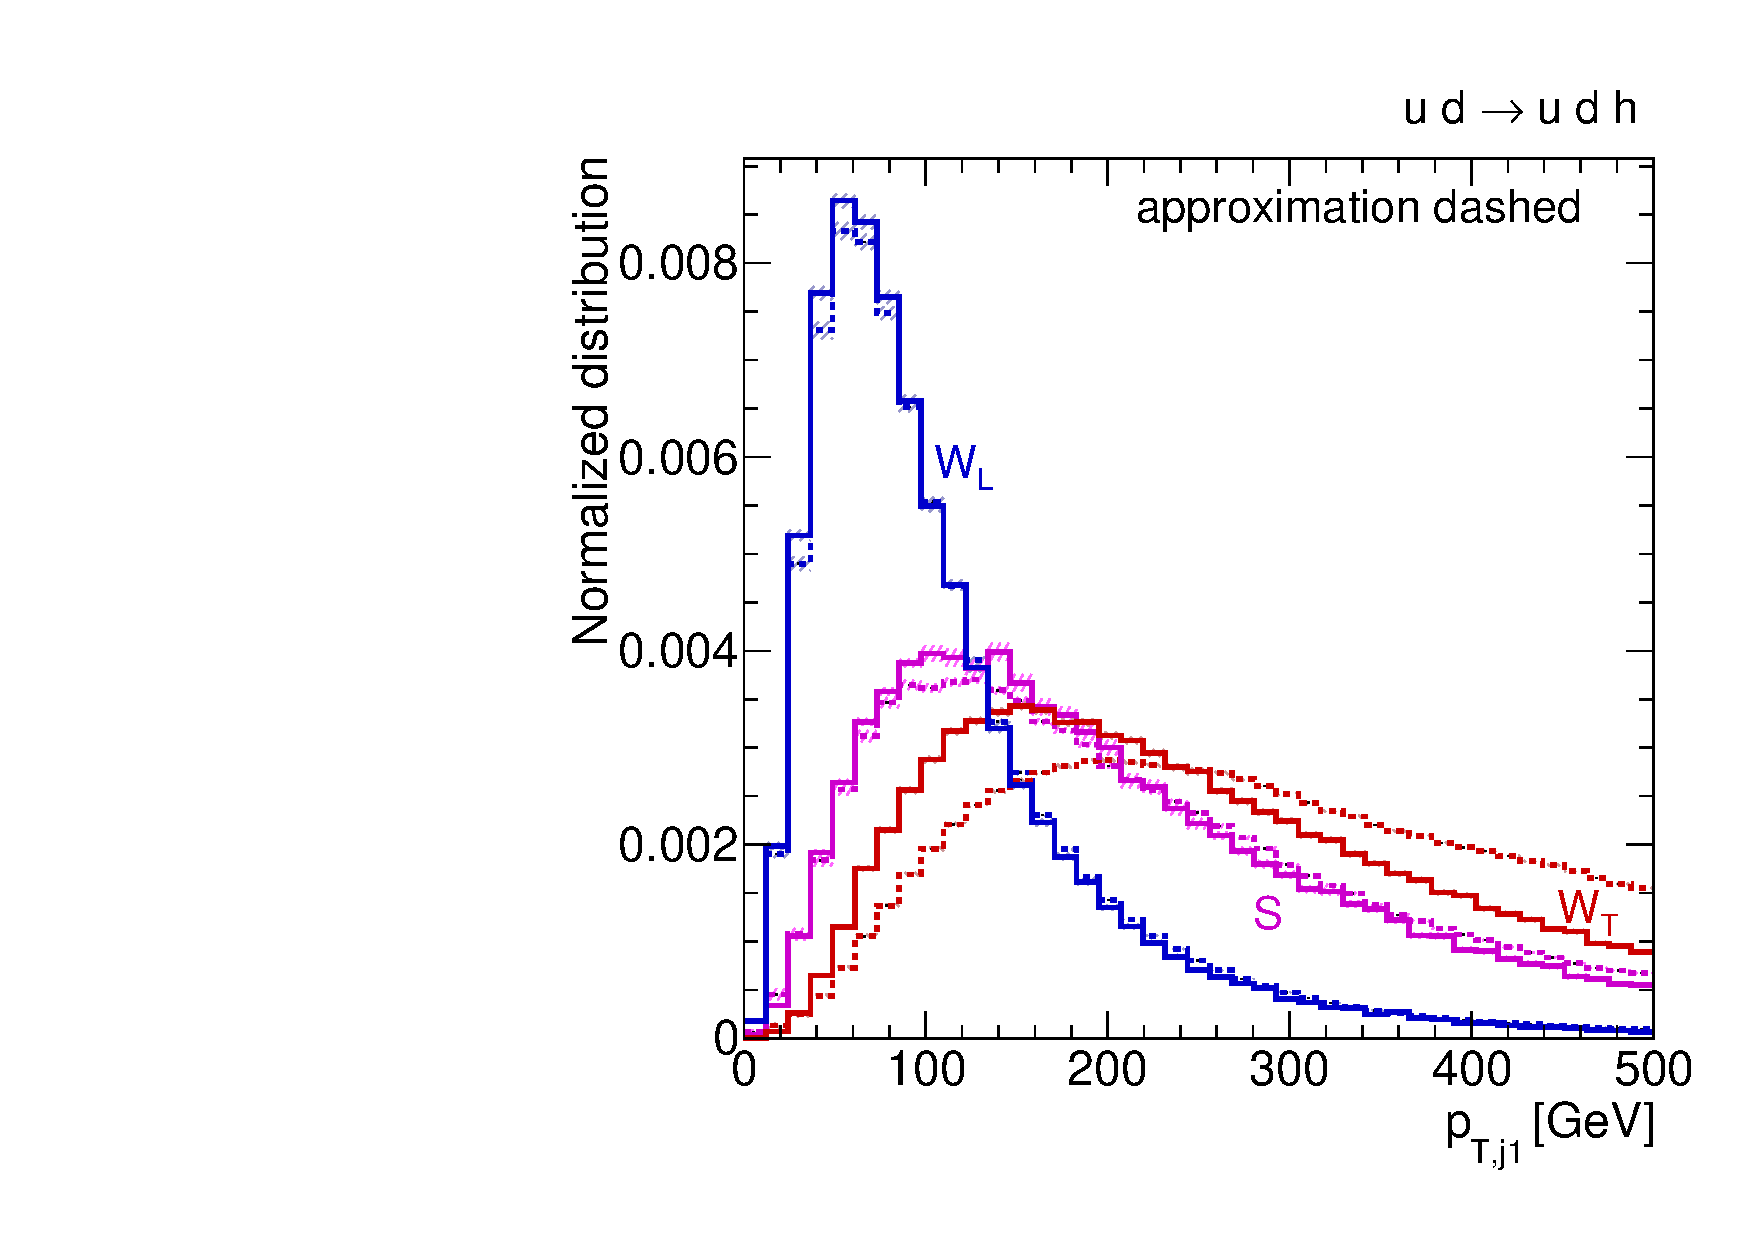
\includegraphics[width=0.43\textwidth]{fig/validity/WBF_ESA.pdf}
  \caption{Normalized WBF distributions of the tagging jets in the SM with
  a heavy Higgs, $m_h = 1$~TeV. Scalar mediators are compared to
  longitudinal and transverse $W$ bosons following
  Ref.~\cite{polarized_ww}.
  The dotted lines give the corresponding predictions of the effective
  $W$ and scalar approximations, Eq.\;\eqref{eq:splittings}.}
  \label{fig:validity_effective_scalar}
\end{figure}
%------------------------------------------------------------



%%%%%%%%%%%%%%%%%%%%%%%%%%%%%%%%%%%%%%%%%%%%%%%%%%%%%%%%%%%%
\subsection{Which observables to study}
%%%%%%%%%%%%%%%%%%%%%%%%%%%%%%%%%%%%%%%%%%%%%%%%%%%%%%%%%%%%

%------------------------------------------------------------
\begin{figure}[t]
%  \centering
  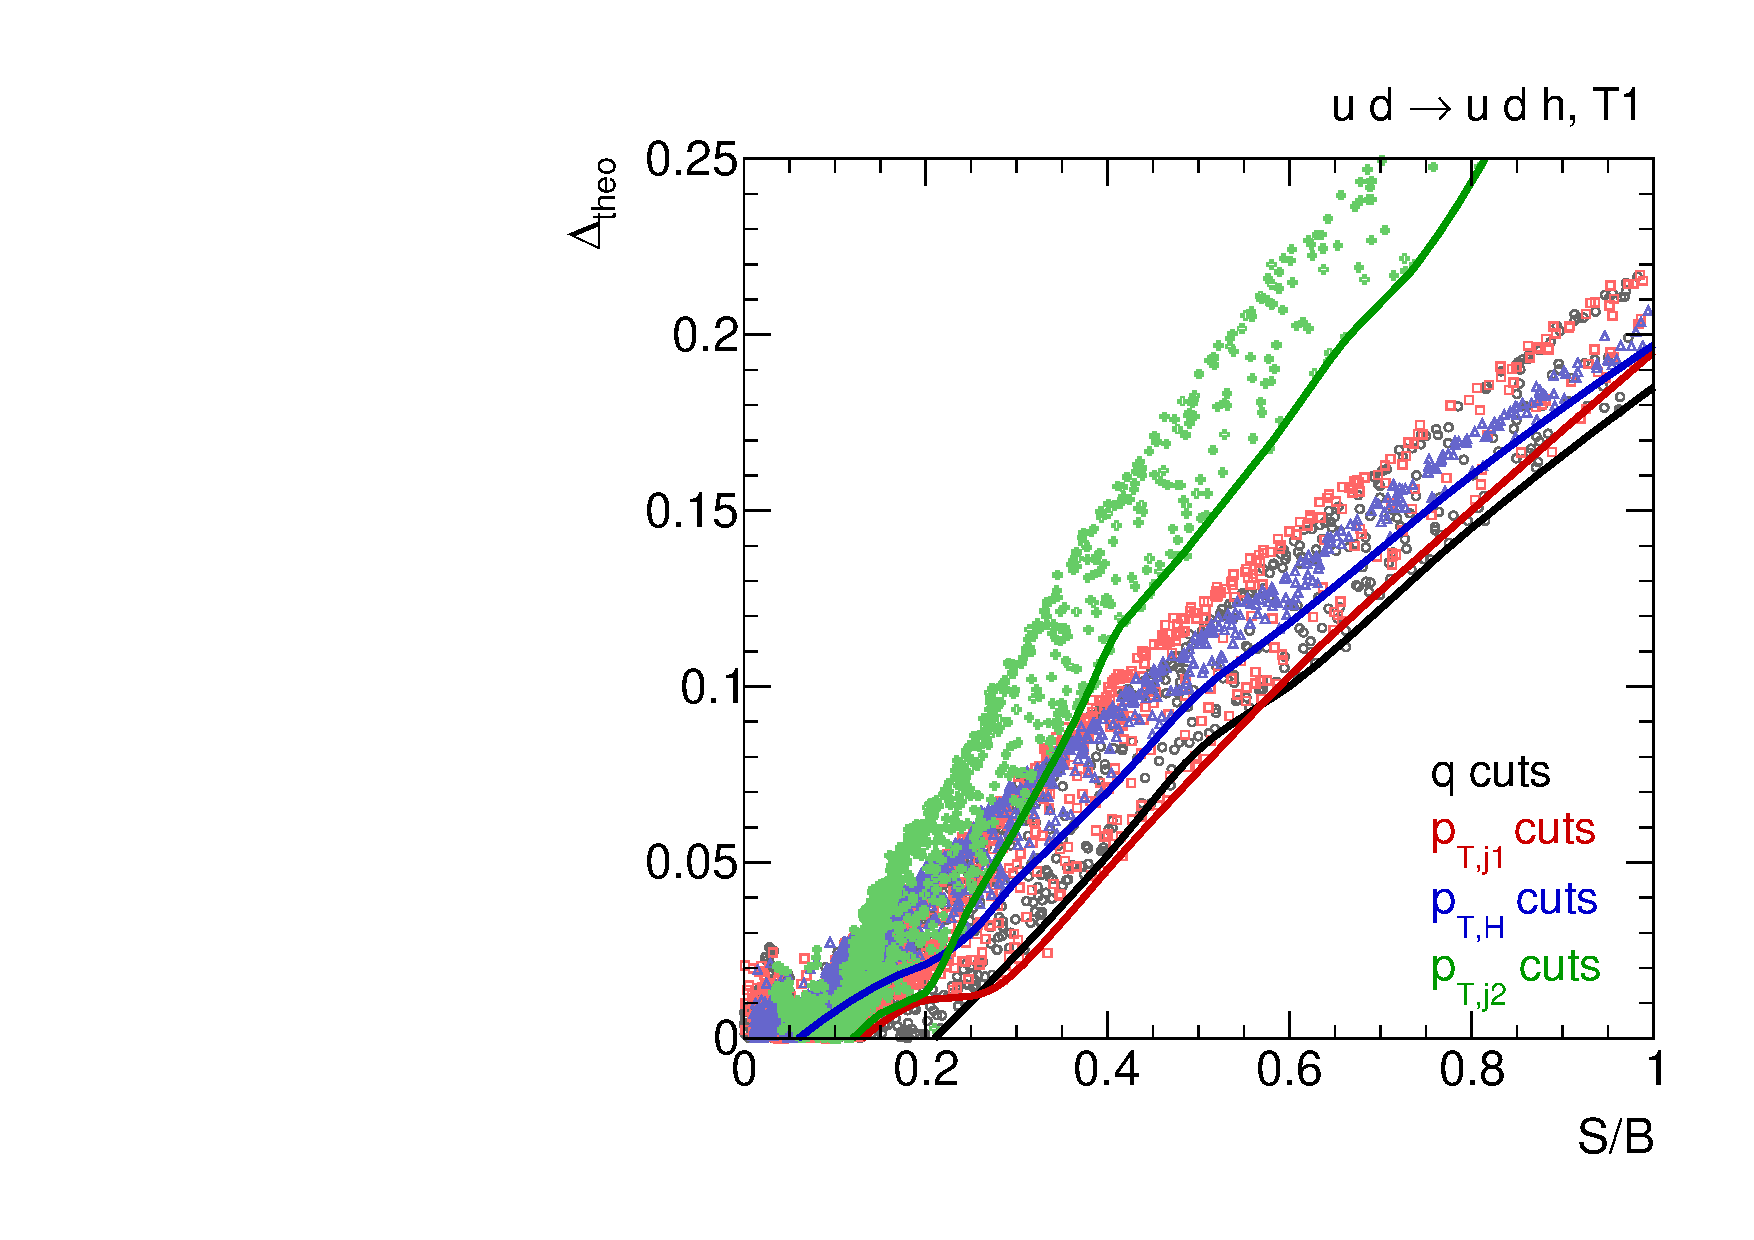
\includegraphics[width=0.43\textwidth]{fig/validity/WBF_cuts_T1_SB.pdf}
  \hspace*{0.05\textwidth}
  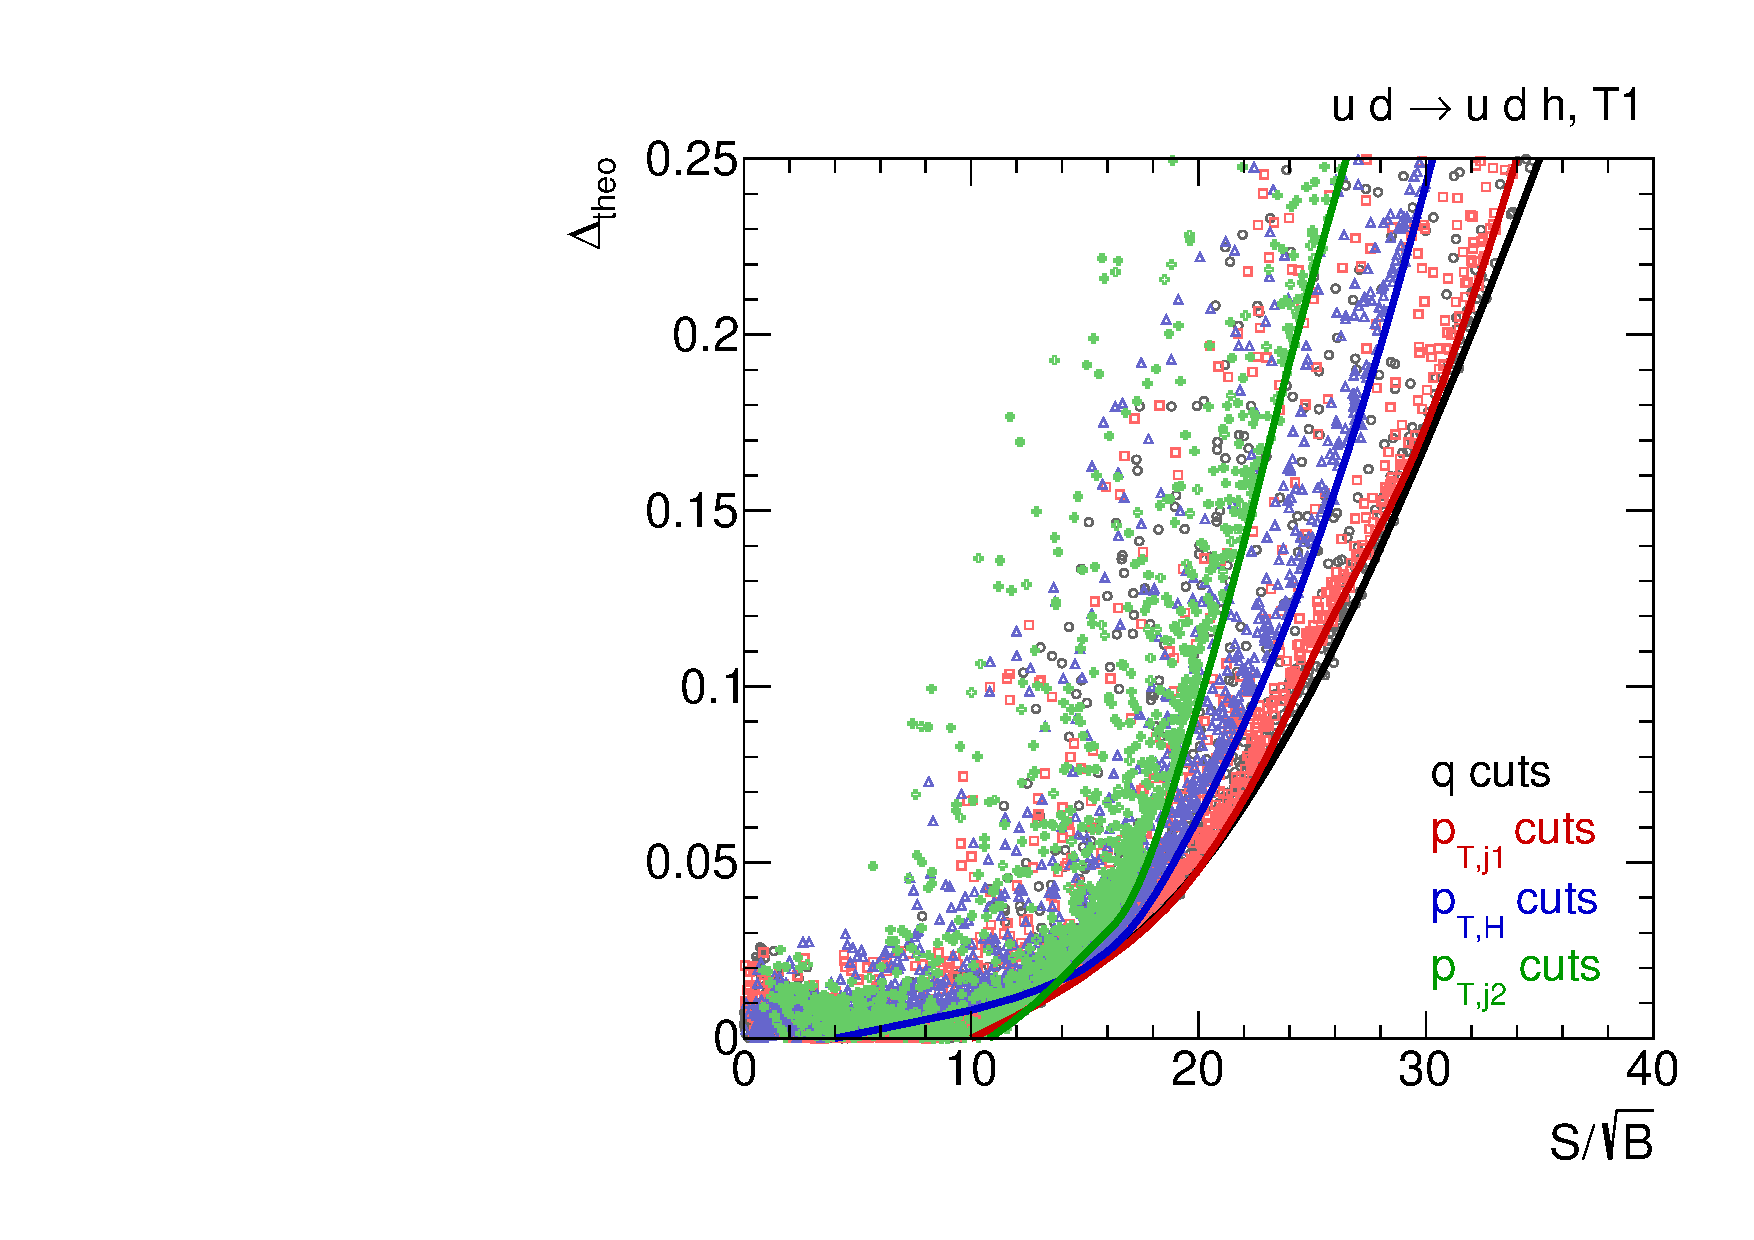
\includegraphics[width=0.43\textwidth]{fig/validity/WBF_cuts_T1_SsqrtB.pdf}
  \caption{Experimental reach in systematics-driven and
    statistics-driven channels vs theoretical uncertainties of the
    dimension-6 description. Each point corresponds to a window
    $x_\text{min,max}$ in one of the four momentum observables that leaves a signal
    cross section of at least 20~fb.}
  \label{fig:validity_cuts}
\end{figure}
%------------------------------------------------------------

Now that it is clear that we cannot further improve the agreement
between the vector triplet and its dimension-6 approximation by adding
a heavy scalar as a simplified model, we go back to the original
problem: how can we best use the dimension-6 approximation for limit
setting, and do the shortcomings shown in
Fig.~\ref{fig:validity_squared_separate} harm this approach?

We know that in our LHC analysis we should avoid angular correlations
of the tagging jets, like $\Delta \eta_{jj}$ or $\Delta
\phi_{jj}$. Instead, we can use momentum-related kinematic variables
like
%
\begin{align}
 x \in \left\{  q, \, p_{T,j_1}, \, p_{T,j_2}, \, p_{T,h} \right\} \; .
\label{eq:variables}
\end{align}
%
An acceptance cut $x > x_\text{min}$ on any of those variables
projects out the interesting phase-space regions, while the cut $x <
x_\text{max}$ ensures the validity of an effective theory
description. If $x_\text{min} > x_\text{max}$ the dimension-6
description is not useful. For each window $x_\text{min,max}$ we can
compute the contribution to the theoretical uncertainty
%
\begin{align}
  \Delta_\text{theo} (x_\text{min,max}) 
= \left| \frac {\sigma_\text{D6} - \sigma_\text{full}} {\sigma_\text{full}} \right| \; ,
\label{eq:err_th}
\end{align} 
%
as well as the statistics-driven and systematics-driven significances
%
\begin{align}
  \frac{S}{B} (x_\text{min,max}) 
= \left| \frac {\sigma_\text{full} - \sigma_\text{SM}} {\sigma_\text{SM}} \right| 
\qquad \text{and} \qquad 
  \frac{S}{\sqrt{B}} (x_\text{min,max}) 
= \sqrt{L} \, \left| \frac {\sigma_\text{full} - \sigma_\text{SM}} {\sqrt{\sigma_\text{SM}}} \right| \; ,
\label{eq:err_ex}
\end{align}
%
where $L = 30~\ifb$ is used as a toy number.

The question is for which
observable $x$ we find the largest $S/B$ and $S/\sqrt{B}$ values while
keeping $\Delta_\text{theo}$ small.  In Fig.~\ref{fig:validity_cuts} we show
the correlations between theoretical uncertainty and experimental
reach for the variables defined in Eq.\;\eqref{eq:variables} for a
parton-level analysis as defined in Eq.\;\eqref{eq:def_wbf}. We see
that the momentum transfer $q$ or the leading tagging jet's
$p_{T,j_1}$ lead to the envelopes with the highest significance for a
given theoretical uncertainty $\Delta_\text{theo}$. This indicates
that the leading tagging jet's transverse momentum is the best way of
experimentally accessing the momentum flow through the hard process,
at least for the hard parton-level process with only two tagging
jets.





%%%%%%%%%%%%%%%%%%%%%%%%%%%%%%%%%%%%%%%%%%%%%%%%%%%%%%%%%%%%
\section{Summary}
\label{sec:validity_summary}
%%%%%%%%%%%%%%%%%%%%%%%%%%%%%%%%%%%%%%%%%%%%%%%%%%%%%%%%%%%%

An effective field theory for the Higgs sector offers a theoretically
well-defined, efficient, and largely model-independent language to
analyze extensions of the Standard Model in both rate measurements and
kinematic distributions. A fit of dimension-6 operators to LHC Higgs
measurements works fine~\cite{Corbett:2015ksa} and constitutes the
natural extension of the Higgs couplings analyses of Run~I.  Most of
the relevant higher-dimensional operators correspond to simple
coupling modifications, supplemented by four operators describing new
Lorentz structures in the Higgs coupling to weak
bosons~\cite{Corbett:2015ksa}.

In this paper we have studied the validity of this approach from the
theoretical side.  We know that at the LHC a clear hierarchy of
electroweak and new physics scales cannot be guaranteed, the question
is whether dimension-6 operators nevertheless capture the
phenomenology of specific UV-complete theories with sufficient
accuracy.  We have systematically compared a singlet Higgs portal
model, a two-Higgs doublet model, scalar top partners, and a heavy
vector triplet to their dimension-6 EFT descriptions, based on the
linear realization of electroweak symmetry breaking with a Higgs
doublet.  We have analyzed the main Higgs production and decay
signatures, covering rates as well as kinematic distributions.\medskip

We have found that the dimension-6 operators provide an adequate
description in almost all realistic weakly coupled scenarios. Shifts
in the total rates are well described by effective operators.
Kinematic distributions typically do not probe weakly interacting new
physics with sufficient precision in the high-energy tails to
challenge the effective operator ansatz.  This is obvious for the
extended scalar models, where new Lorentz structures and
momentum-dependent couplings with dramatic effects in LHC
distributions only appear at the loop level.  A loop-suppressed
effective scale suppression $E^2/(4 \pi \Lambda)^2$ has to be compared
with on-shell couplings modifications proportional to $v^2/\Lambda^2$.
Only phase space regions probing energies around $4 \pi v \approx
3$~TeV significantly constrain loop contributions in the Higgs sector
and eventually lead to breakdown of the effective field theory. In
turn, a simple dimension-6 descriptions will capture all effects that
are expected to be measurable with sufficient statistics at the LHC
Run II.  On the other hand, the vector triplet model shows that
modifications of the gauge sector can generate effects in LHC
kinematics at tree level. However, we again find that for weakly
interacting models and phenomenologically viable benchmark points they
are described well by an appropriate set of dimension-6
operators.\medskip

%-----------------------------------------------------------
\begin{table}[t] \renewcommand{\arraystretch}{1.2} \centering
\begin{tabular}{ll c ccc} \toprule Model & Process &\hspace*{1em}&
\multicolumn{3}{c}{EFT failure} \\ \cmidrule{4-6} & && resonance &
kinematics & matching \\ \midrule singlet & on-shell $h \to 4 \ell$,
WBF, $Vh$, \dots && & & \largex \\ & off-shell WBF, \dots && &
\brlargex & \largex \\ & $hh$ && \largex & \largex & \largex \\ 2HDM &
on-shell $h \to 4 \ell$, WBF, $Vh$, \dots && & & \largex \\ &
off-shell $h \to \gamma \gamma$, \dots && & \brlargex & \largex \\ &
$hh$ && \largex & \largex & \largex \\ top partner & WBF, $Vh$ && & &
\largex \\ vector triplet & WBF && & \brlargex & \largex \\ & $Vh$ &&
\largex & \brlargex & \largex \\ \bottomrule
\end{tabular}
 \caption{Possible sources of failure of dimension-6 Lagrangian at the
LHC.  We use parentheses where deviations in kinematic distributions
appear, but are unlikely to be observed in realistic scenarios.}
 \label{tab:differences}
\end{table}
%-----------------------------------------------------------


Three sources for a possible breakdown of the dimension-6 description
are illustrated in Tab.~\ref{tab:differences}\footnote{Forcing the EFT
approach into a spectacular breakdown was the original aim of this
paper, but to our surprise this did not happen.}: First, the EFT
cannot describe light new resonances. Such a signature at the LHC
would be an obvious signal to stop using the EFT and switch to
appropriate simplified models.  Second, selected kinematic
distributions fail to be described by the dimension-6 Lagrangian, in
particular for Higgs pair production.  Deviations in the high-energy
tails of WBF and Higgs-strahlung distributions on the other hand are
too small to be relevant in realistic weakly coupled scenarios. These
two cases do not threaten LHC analyses in practice.

The third issue with the dimension-6 EFT description is linked to
matching in the absence of a well-defined scale hierarchy.  Even with
only one heavy mass scale in the Lagrangian, the electroweak VEV
together with large couplings can generate several new physics scales,
defined by the masses of the new particles.  A linear EFT description,
which is justified by the SM-like properties of the newly discovered
Higgs boson, should in principle be matched in the phase where the
electroweak symmetry is unbroken. Such a procedure is blind to
additional scales induced by the electroweak VEV, potentially leading
to large errors in the dimension-6 approximation.  Including
$v$-dependent terms in the Wilson coefficients, which corresponds to
matching in the broken phase, can significantly improve the EFT
performance. We have explicitly demonstrated this for all the models
considered in this paper.

None of these complications with the dimension-6 description presents
a problem in using effective operators to fit LHC Higgs data.  They
are purely theoretical issues that need to be considered for the
interpretation of the results.


%%%%%%%%%%%%%%%%%%%%%%%%%%%%%%%%%%%%%%%%

While a dimension-6 Higgs analysis at the LHC cannot be considered the
leading part of a consistent effective theory, it describes the
effects of weakly interacting extensions of the Higgs-gauge sector very
well~\cite{too_long}. In this brief study we have answered two practical
question concerning such a dimension-6 analysis for Run~II.

First, a priori it is not clear if squared dimension-6 terms should be
included in calculations. We have studied two particularly challenging
parameter points of a vector triplet model for $Vh$ production and for
weak-boson-fusion Higgs production. For both processes we find that
the dimension-6 squared term avoids negative rate predictions in the
$m_{Vh}$ or $p_{T,V}$ distributions of $Vh$ production and in the
$p_{T,j_1}$ distribution of weak boson fusion. Even for cases with a
constructive interference between the dimension-6 and the Standard
Model contributions, it turns out that including the dimension-6
squared term improves the agreement of kinematic distributions between
the full model and the dimension-6 approximation. Ultimately, this
translates into a better agreement in the expected exclusion
limits\footnote{Similar conclusions in a different framework have recently
been published in Ref.~\cite{gino}.}.

Second, we have attempted to improve the agreement between the full
model and our approximation by using a simplified model. The only
significantly simpler model than a mixing gauge extension is an
extended scalar sector. While the corresponding deviations between the
full model and the dimension-6 approximation are phenomenologically
hardly relevant, we find that such an additional scalar improves the
modelling of kinematic distributions of the kind $m_{Vh}$ and
$p_{T,j_1}$ where the dimension-6 description breaks down. However,
this comes at the cost of significant deviations in the dominant
interference terms. Moreover, once we include angular correlations
like $\Delta \eta_{jj}$ or $\Delta \phi_{jj}$ in weak boson fusion,
the simplified model fails badly. The difference can be traced to the
divergence structure of the corresponding splittings.

Seeing that the dimension-6 approach is still the better simple model
to describe new physics in WBF distributions, we have finally analyzed
which phase-space regions provide an interesting window to new physics
while being well described by the dimension-6 approximation.  We have
demonstrated that the leading tagging jet's $p_T$ distribution is
particularly suited for such a search for new physics.
